% Paquets généraux
\documentclass[a4paper,12pt,titlepage,twoside]{article}
\usepackage[T1]{fontenc}
\usepackage[utf8]{inputenc}
\usepackage[french]{babel}
\usepackage{subcaption}
\addto\captionsfrench{%
  \renewcommand{\tablename}{Tableau}%
}
\usepackage[gen]{eurosym}
%\usepackage[dvips]{graphicx}
\usepackage{minted}
\usepackage{fancyhdr}
\usepackage{pdfpages} 
\usepackage{multido}
\usepackage{hyperref}
\usepackage{textcomp}
\usepackage{schemabloc}
%\usepackage[bitstream-charter]{mathdesign}
\usepackage{array}
\newcolumntype{P}[1]{>{\centering\arraybackslash}p{#1}}
\usepackage[shortlabels]{enumitem}
\usepackage[framemethod=TikZ]{mdframed}

\newcommand{\id}{71}
\newcommand{\nom}{Théorie des mécanismes}
\newcommand{\sequence}{04}
\newcommand{\nomsequence}{Liaisons entre les solides}
\newcommand{\num}{02}
\newcommand{\type}{KH}
\newcommand{\descrip}{Liaisons équivalentes, hyperstatisme, liaisons en série et en parallèle, théorie des graphes}
\newcommand{\competences}{B2-12: Proposer une modélisation des liaisons avec leurs caractéristiques géométriques. \\ &  B2-13: Proposer un modèle cinématique paramétré à partir d'un système réel, d'une maquette numérique ou d'u \\ &  B2-17: Simplifier un modèle de mécanisme. \\ &  B2-18: Modifier un modèle pour le rendre isostatique. \\ &  C1-04: Proposer une démarche permettant d'obtenir une loi entrée-sortie géométrique.  \\ &  C2-05: Caractériser le mouvement d'un repère par rapport à un autre repère. \\ &  C2-06: Déterminer les relations entre les grandeurs géométriques ou cinématiques. }
\newcommand{\nbcomp}{7}
\newcommand{\systemes}{}
\newcommand{\systemesnum}{}
\newcommand{\systemessansaccent}{}
\newcommand{\ilot}{2}
\newcommand{\ilotstr}{02}
\newcommand{\dossierilot}{\detokenize{Ilot_02 }}

%\usepackage{style}
\usepackage{bodegraph}
\usepackage{rpcinematik}
\usepackage[locale = FR]{siunitx}
\usepackage{caption}
\newcommand{\institute}{Lycée Dorian}

\usepackage{listings}
\usepackage{fancyvrb}
\usepackage{color}
\usepackage{xcolor}
\usepackage{colortbl}
\usepackage{helvet}
\usepackage[frenchmath]{newtxsf} % for sans serif symbols
\renewcommand{\familydefault}{\sfdefault}
%\usepackage{amsfonts}
%\usepackage{amsmath}
%\usepackage{lmodern}
\usepackage{mathastext}
%\usepackage{xspace}
\usepackage{varioref}
\usepackage{tabularx}
%\usepackage{floatflt}
\usepackage{graphics}
\usepackage{wrapfig}
\usepackage{textcomp}
\usepackage{tikz,tkz-tab}
\usepackage[european resistor, european voltage, european current]{circuitikz}
\usepackage{wrapfig}
\usepackage{gensymb}
\usepackage[percent]{overpic}
\usetikzlibrary{babel}
\usepackage{ifthen}
\usepackage{cancel}
\usepackage{etoolbox}
\usepackage{multirow}
%\usepackage{boxedminipage}
\definecolor{gris25}{gray}{0.75}
\definecolor{bleu}{RGB}{18,33,98}
\definecolor{bleuf}{RGB}{42,94,171}
\definecolor{bleuc}{RGB}{231,239,247}
\definecolor{bleum}{RGB}{160,195,226}
\definecolor{rougef}{RGB}{185,18,27}
\definecolor{rougec}{RGB}{255,188,204}%255,230,231
\definecolor{vertf}{RGB}{103,126,82}
\definecolor{vertc}{RGB}{220,255,191}
\definecolor{forestgreen}{rgb}{0.13,0.54,0.13}
\definecolor{blcr}{rgb}{0.59,0.69,0.84}
\definecolor{blfr}{rgb}{0.32,0.51,0.75}
\definecolor{orfr}{rgb}{0.90,0.42,0.15}
\definecolor{orcr}{rgb}{0.90,0.65,0.50}
\definecolor{orangef}{rgb}{0.659,0.269,0.072}
\definecolor{orange}{rgb}{0.58,0.35,0.063}
\definecolor{orangec}{rgb}{0.43,0.32,0.25}
\definecolor{rcorrect}{rgb}{0.6,0,0}
\definecolor{sequence}{rgb}{0.75,0.75,0.75}
\definecolor{competences}{rgb}{0.61,0.73,0.35}
\definecolor{rose}{HTML}{ff00ff}
\definecolor{grisf}{HTML}{222222}
\definecolor{grisc}{HTML}{636363}
\definecolor{normal}{HTML}{4087c4}
\definecolor{info}{HTML}{5bc0de}
\definecolor{success}{RGB}{92,184,92}
\definecolor{warning}{RGB}{240,173,78}
\definecolor{danger}{RGB}{217,83,79}
\hypersetup{                    % parametrage des hyperliens
    colorlinks=true,                % colorise les liens
    breaklinks=true,                % permet les retours à la ligne pour les liens trop longs
    urlcolor= blfr,                 % couleur des hyperliens
    linkcolor= orange,                % couleur des liens internes aux documents (index, figures, tableaux, equations,...)
    citecolor= forestgreen                % couleur des liens vers les references bibliographiques
    }

\newcolumntype{M}[1]{>{\centering\arraybackslash}m{#1}}
\definecolor{codegreen}{rgb}{0,0.6,0}
\definecolor{codegray}{rgb}{0.5,0.5,0.5}
\definecolor{codepurple}{rgb}{0.58,0,0.82}
\definecolor{backcolour}{rgb}{0.95,0.95,0.92}

\lstdefinestyle{mystyle}{
    backgroundcolor=\color{backcolour},   
    commentstyle=\color{codegreen},
    keywordstyle=\color{magenta},
    numberstyle=\tiny\color{codegray},
    stringstyle=\color{codepurple},
    basicstyle=\ttfamily\footnotesize,
    breakatwhitespace=false,         
    breaklines=true,                 
    captionpos=b,                    
    keepspaces=true,                 
    numbers=left,                    
    numbersep=5pt,                  
    showspaces=false,                
    showstringspaces=false,
    showtabs=false,                  
    tabsize=2
}

\lstset{style=mystyle}

% Mise en page
\pagestyle{fancy}

\setlength{\hoffset}{-18pt}
\setlength{\oddsidemargin}{0pt} 	% Marge gauche sur pages impaire2s
\setlength{\evensidemargin}{0pt} 	% Marge gauche sur pages paires
\setlength{\marginparwidth}{00pt} 	% Largeur de note dans la marge
\setlength{\headwidth}{481pt} 	 	% Largeur de la zone de tête (17cm)
\setlength{\textwidth}{481pt} 	 	% Largeu\textbf{r de la zone de texte (17cm)
\setlength{\voffset}{-18pt} 		% Bon pour DOS
\setlength{\marginparsep}{7pt}	 	% Séparation de la marge
\setlength{\topmargin}{-30pt} 		% Pas de marge en haut
\setlength{\headheight}{55pt} 		% Haut de page
\setlength{\headsep}{20pt} 		% Entre le haut de page et le texte
\setlength{\footskip}{30pt} 		% Bas de\textbf{ page + séparation
\setlength{\textheight}{700pt} 		% Hauteur de l'icone zone de texte (25cm)
\setlength\fboxrule{1 pt}
\renewcommand{\baselinestretch}{1}
\setcounter{tocdepth}{1}
\newcommand{\cadre}[2]
{\fbox{
  \begin{minipage}{#1\linewidth}
   \begin{center}
    #2\\
   \end{center}
  \end{minipage}
 }
}

\newcommand{\repon}[1]
{
~\ \\
\begin{tabular}{|m{\linewidth}|}
 \hline
\multido{}{#1}{\\ \hline}
\end{tabular}
}


\newcommand{\objectif}[1]{
\mdfsetup{%
frametitle={%
\tikz[baseline=(current bounding box.east),outer sep=0pt]
\node[anchor=east,rectangle,fill=bleum]
{\strut Objectif~};}}
\mdfsetup{innertopmargin=10pt,linecolor=bleum,%
linewidth=2pt,topline=true,%
frametitleaboveskip=\dimexpr-\ht\strutbox\relax
}
\begin{mdframed}[]\relax%
#1
\end{mdframed}}


\newcounter{num_quest} \setcounter{num_quest}{0}
\newcounter{num_rep} \setcounter{num_rep}{0}
\newcounter{num_cor} \setcounter{num_cor}{0}

\newcommand{\feuilleDR}[1]{
	\begin{tikzpicture}
		\draw[gray!30](0,0)grid[step=0.5cm](\linewidth,#1);
	\end{tikzpicture}
}

%\newcommand{\question}[1]{\refstepcounter{num_quest}\par
%~\ \\ \parbox[t][][t]{0.15\linewidth}{\textbf{Question \arabic{num_quest}}}\parbox[t][][t]{0.85\linewidth}{#1\label{q\the\value{num_quest}}}\par
%}

\newcommand{\question}[1]{\refstepcounter{num_quest}\par
~\ \\ \textbf{Question \arabic{num_quest} : }#1\label{q\the\value{num_quest}}\par
}

\newcommand{\posetafigure}[3]{
\begin{figure}[ht!]
 \begin{center}
  \includegraphics[width=#2\linewidth]{img/#1}
 \end{center}
 \caption{\label{#1} #3}
\end{figure}}

\newcommand{\goforum}{
\begin{figure}

\end{figure}
\begin{center}
 
\includegraphics[width=0.7\linewidth]{../../../img/go_forum}
\end{center}
\label{go_forum}
\caption{J'pète les plombs}
\end{figure}}

\newcommand{\reponse}[4][1]
{\noindent
\parbox{\textwidth}{
\rule{\linewidth}{.5pt}\\
\textbf{Question\ifthenelse{#1>1}{s}{} \multido{}{#1}{%
\refstepcounter{num_rep}\ref{q\the\value{num_rep}} }:} ~\ \\
\ifdef{\public}{#3 \ifthenelse{#2>0}{~\ \\ 	\feuilleDR{#2}}}{#4}
}}

\newcommand{\cor}
{\refstepcounter{num_cor}
\noindent
\rule{\linewidth}{.5pt}
\textbf{Question \arabic{num_cor}:} \\
}

\newcommand{\finsujet}
{
    \begin{center}
    \Large{FIN}
    \end{center}

    \cleardoublepage

    \ifdef{\public}{\pagestyle{docreponse}}{\pagestyle{correction}}

    \ifdef{\public}{
        \begin{tikzpicture} 
            \draw (0,0) rectangle (2,2);
            \draw (0,0) -- (2,2);
            \draw (1.5,0.5) node {\large 20};
            \draw (2.5,0) rectangle (16,2);
            \draw (4.5,1.7) node {\large Commentaires:};
        \end{tikzpicture}
    }
    ~\ \\
}


%\newcommand{\repcarre}[2]
%{
%~\ \\
%\begin{tikzpicture}
%\draw [fill=white] (0,0) rectangle +(\linewidth,#1);
%\node[align=left] at (1.1,#2-0.3) {\textbf{Question #1:}};
%\end{tikzpicture}
%}

\newcommand{\titre}[1]
{\begin{center}
\cadre{0.8}{\huge #1} 
\end{center}
}


%Définition des torseurs :
\newcommand{\torseur}[2]{\left\{\mathcal{#1}_{#2} \right\}}
\newcommand{\torseurh}[3]{\left\{\genfrac{}{}{0pt}{0}{#1}{#2}\right\}_{#3}}
\newcommand{\torseurv}[8]{\left\{
\begin{matrix}
#1 & #4 \\ #2 & #5 \\ #3 &#6
\end{matrix}
\right\}_{{#7},{#8}}}

%Définition des torseurs :
%\newcommand{\torseur}[2]{\left \{\mbox{\relsize{2}{$\mathcal {#1}$}\relsize{-2}}\phantom{}_{\mbox{\scriptsize $#2$}} \right \}}
%\newcommand{\torseurh}[3]{\left\{\genfrac{}{}{0pt}{0}{#1}{#2}\right\}_{#3}}
%\newcommand{\torseurv}[8]{
%\left\{\begin{array}{@{}c|c@{}} #1 & #4 \\ #2 & #5 \\ #3 & #6 \end{array} \right\}_{#7,#8}
%}
\newcommand{\derivee}[2]{\left.\dfrac{\d #1}{\d t}\right|_{#2}}
\newcommand{\tripleint}{\int\!\!\!\!\!\int\!\!\!\!\!\int}

% Notation cinématique et statique
\newcommand{\cinematique}[2]{\mbox{#1}/\mbox{#2}}
\newcommand{\statique}[2]{\mbox{#1}\rightarrow\mbox{#2}}
\newcommand{\moment}[3]{\vv {#1}_{\scriptsize{#3}}(#2)}
\newcommand{\resultante}[2]{\vv {#1}_{\scriptsize{#2}}}


%Commande de base
\newcommand{\jo}{\left(j\omega\right)} % j \omega dans l'analyse fréquentielle
\newcommand{\tl}{\xrightarrow{\mathcal{L}}} % transformée de laplace sur fleche
\newcommand{\tli}{\xrightarrow{\mathcal{L}^{-1}}} % transformée inverse de laplace sur fleche
\renewcommand{\d}[1][]{\mathrm{d#1}}
\newcommand{\dd}[1][]{\mathrm{d#1}}
\newcommand{\vect}[2]{{#1}\wedge{#2}}
\newcommand{\base}[3]{(\vec #1,\vec #2,\vec #3)}
\newcommand{\vectbase}[4]{{\vphantom{\left| \begin{matrix}
#1\\#2\\#3 \end{matrix} \right|}}_{#4}{\left| \begin{matrix}
#1\\#2\\#3 \end{matrix} \right.}}
%Pour avoir les paragraphes sous la forme I, II, III
\renewcommand{\thesection}{\Roman{section}}
\setcounter{secnumdepth}{3}
\renewcommand{\Frlabelitemii}{$\bullet$}

% En tête et pied de page
\lhead{\nom}
\rhead{
\includegraphics[width=2cm]{../../../img/logo}}
\lfoot{\auteurun,\ \auteurdeux}
\cfoot{Page \thepage}

\fancypagestyle{docreponse}{%
  \fancyhf{}
  \fancyhead[LO]{NOM Prénom: .............................}
  \rhead{
\includegraphics[width=2cm]{../../../img/logo}\hspace{2pt}}
  \ifdef{\auteurdeux}{\lfoot{\auteurun,\ \auteurdeux}}{\lfoot{\auteurun}}
  \rfoot{\nom}
  \lfoot{Document réponse}
  \cfoot{Page \thepage}
   }

\fancypagestyle{correction}{%
  \fancyhf{}
  \lhead{\colorbox{danger}{\begin{minipage}{0.65\paperwidth} \textcolor{white}{\textbf{Correction}} \end{minipage}} }
  \rhead{
\includegraphics[width=2cm]{../../../img/logo}}
  \lfoot{Renaud Costadoat, Françoise Puig}
  \rfoot{\colorbox{danger}{\begin{minipage}{0.4\paperwidth} \begin{flushright}\textcolor{white}{\textbf{Correction}}\end{flushright} \end{minipage}} }}

\fancypagestyle{correctioninfo}{%
  \fancyhf{}
  \lhead{\colorbox{danger}{\begin{minipage}{0.65\paperwidth} \textcolor{white}{\textbf{Correction}} \end{minipage}} }
  \rhead{
\includegraphics[width=2cm]{../../../img/logo}}
  \lfoot{Renaud Costadoat, Juliette Genzmer}
  \rfoot{\colorbox{danger}{\begin{minipage}{0.6\paperwidth} \begin{flushright}\textcolor{white}{\textbf{Correction}}\end{flushright} \end{minipage}} }}

\renewcommand{\footrulewidth}{0.4pt}

\usepackage{eso-pic}
\newcommand{\BackgroundPic}{%
\put(0,0){%
\parbox[b][\paperheight]{\paperwidth}{%
\vfill
\begin{center}
\hspace{0.5cm}\vspace{0.5cm}

\includegraphics[width=\paperwidth,height=\paperheight,%
keepaspectratio]{../../../img/fond3}%
\end{center}
\vfill
}}}

\newcommand{\BackgroundPicdeux}{%
\put(25,-30){%
\parbox[b][\paperheight]{\paperwidth}{%
\vfill
\begin{center}
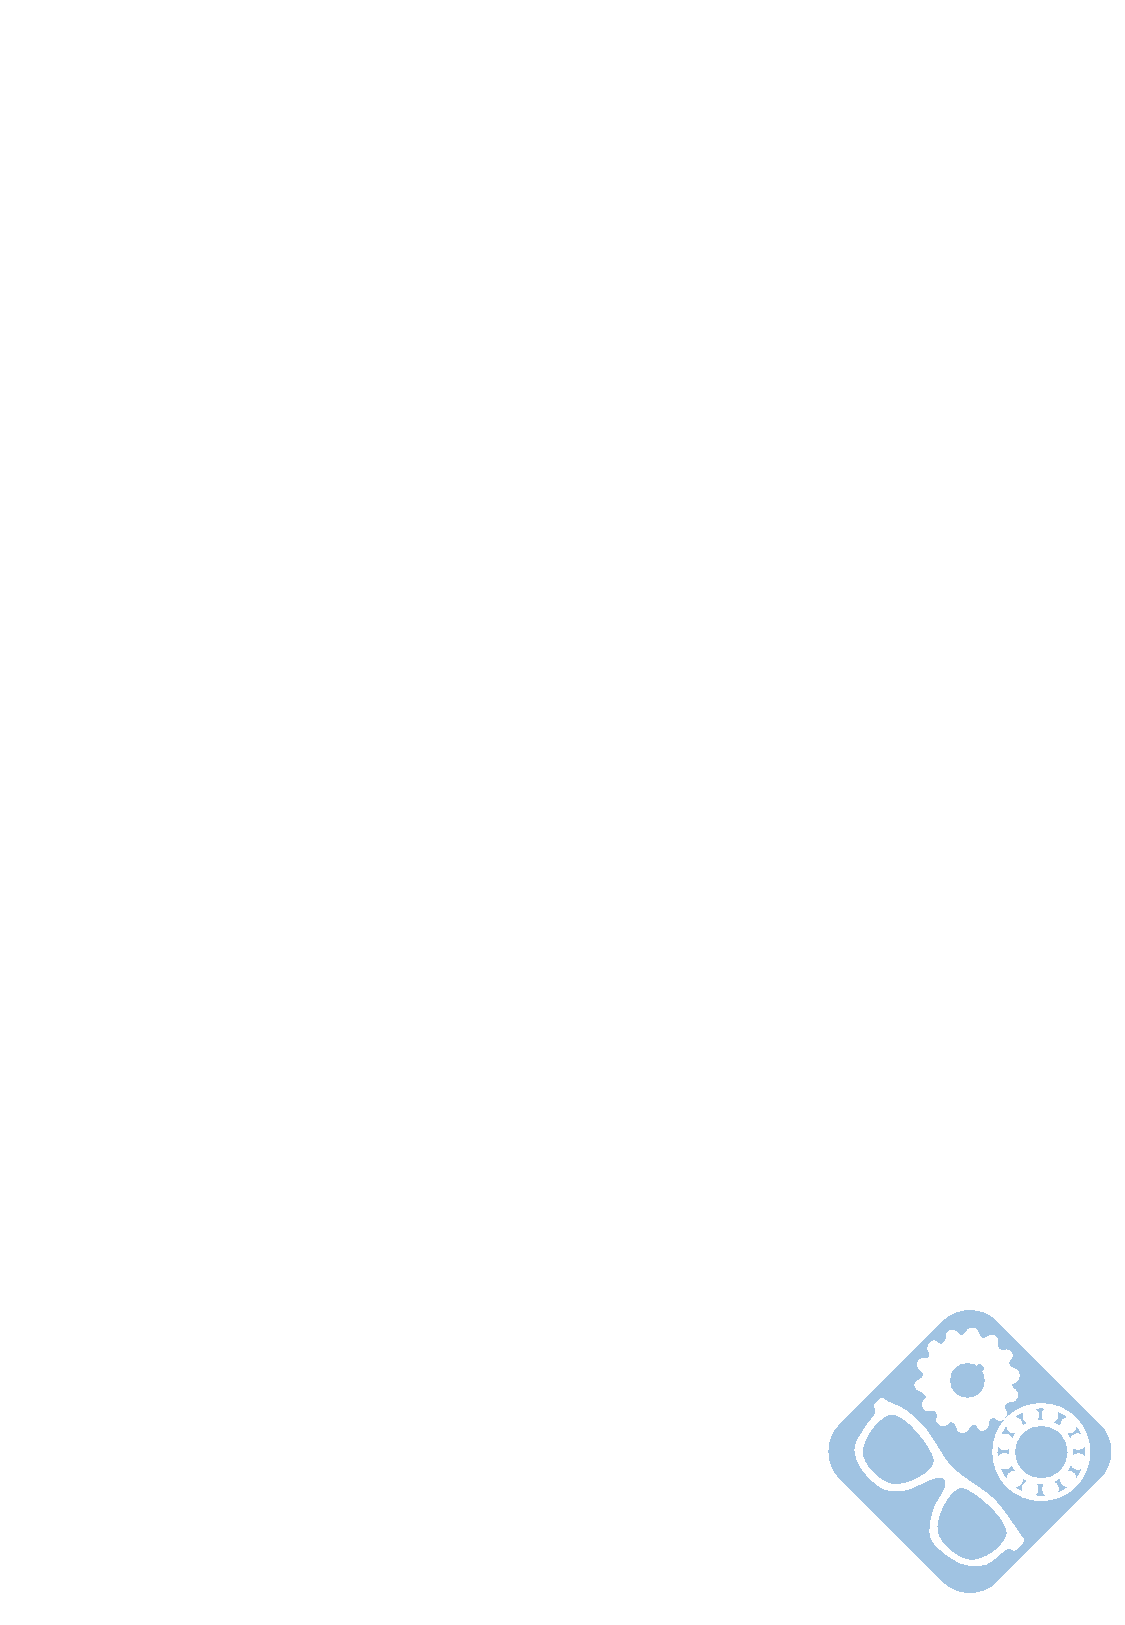
\includegraphics[width=\paperwidth,height=\paperheight,%
keepaspectratio]{../../../img/fond4}%
\end{center}
\vfill
}}}

\begin{document}

\pagestyle{empty}

\AddToShipoutPicture*{\BackgroundPic}


\includegraphics[width=2cm]{../../../img/logo}

\Huge{DS \numero - \sujet}

\vspace{1cm}

\ifdef{\prive}{\begin{center}\colorbox{danger}{\Huge{Avec Correction}}\end{center}}{}

\begin{center}
\centering\huge{PTSI}
\end{center}

\vspace{2cm}


\begin{center}
\centering\Large{\jour}
\end{center}

\vspace{2cm}

\normalsize

\tableofcontents

\newpage

\AddToShipoutPicture{\BackgroundPicdeux}

\pagestyle{fancy}

\begin{center}
\Huge \sujet
\end{center}


\normalsize


\section{Présentation}

\subsection{Contexte}

La houle est constituée de vagues successives nées de l'effet du vent à la surface de la mer et pouvant parfois se propager sur de très longues distances. Il s'agit d'une forme concentrée de l'énergie du vent, elle-même issue de l'énergie solaire, c'est donc une énergie renouvelable dont le potentiel n'est actuellement quasiment pas exploité.

~\

\begin{wrapfigure}[18]{r}{0.65\textwidth}
	\vspace{-0.8cm}
\begin{center}
  \def\svgwidth{0.8\linewidth}
  \input{img/fig01.pdf_tex}
 \end{center}
  \caption{Principe des bouées de type \og Powerbuoy \fg}
\label{fig01}
\end{wrapfigure}

L'énergie produite à partir de la houle est appelée houlomotrice (ou énergie des vagues). Cette énergie est le plus souvent transformée en énergie électrique.

Différents dispositifs pour exploiter cette énergie sont en développement. Même si certains d'entre eux font l'objet d'une commercialisation, aucun n'a réellement atteint le stade de la maturité industrielle, contrairement au domaine de l'énergie éolienne ou solaire.

Le dispositif étudié est une bouée houlomotrice de type \og Powerbuoy \fg (figure \ref{fig01}). Il s'agit d'une structure flottante constituée :

\begin{itemize}
 \item d'un lest, composé de deux parties (lest inférieur et lest supérieur), partie immergée fixe (ou peu mobile) grâce à un système de mouillage (amarrage) au fond marin (non représenté),
 \item d'un flotteur, partie émergeante flottante pouvant coulisser verticalement par rapport au lest.
\end{itemize}

Celui-ci capte l'énergie de la houle en suivant les déplacements verticaux de la surface de la mer, ce qui permet de produire de l'énergie électrique.

\begin{wrapfigure}[9]{l}{0.55\textwidth}
	\vspace{-0.8cm}
  \begin{center}
    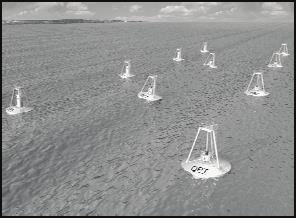
\includegraphics[width=0.7\linewidth]{img/fig02}
  \end{center}
  \caption{Ferme marine}
\label{fig02}
\end{wrapfigure}

Les bouées houlomotrices sont généralement déployées par groupe allant jusqu'à une dizaine d'unités constituant ainsi des "fermes marines" (figure \ref{fig02}). Celles-ci partagent le système d'amarrage des lests ainsi qu'une station sous marine qui permet de collecter l'énergie électrique produite et de l'envoyer au réseau électrique à terre par l'intermédiaire d'un câble sous-marin.

\newpage

Le diagramme SysML des cas d'utilisation en annexe permet de mettre en évidence deux configurations que doit adopter la bouée houlomotrice :

\begin{itemize}
 \item une configuration verticale, avec le lest inférieur complètement immergé, en phase de production d'énergie ;
 \item une configuration horizontale (figure \ref{fig03}), avec le lest inférieur partiellement immergé, en phase d'installation sur zone de production et de retour à terre pour maintenance, par simple
remorquage.
\end{itemize}

\begin{figure}[ht!]
  \begin{center}
    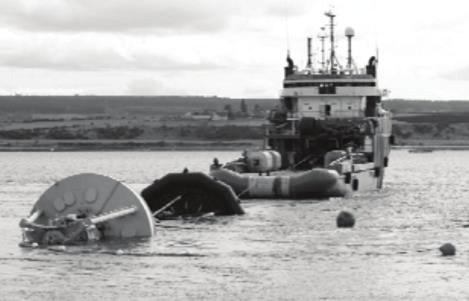
\includegraphics[width=0.32\linewidth]{img/fig03a}
    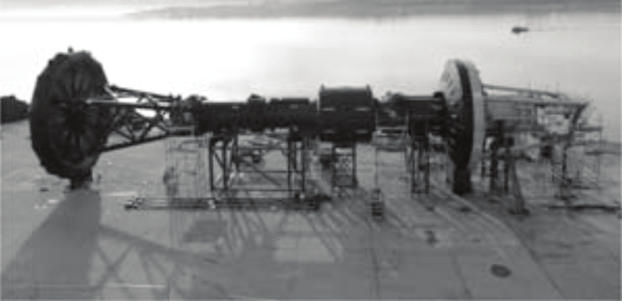
\includegraphics[width=0.32\linewidth]{img/fig03b}
  \end{center}
  \caption{Configuration horizontale pour maintenance et transport}
\label{fig03}
\end{figure}

\vspace{-1cm}

\subsection{Description du système}

Le système d'absorption d'énergie est constitué de deux principaux sous-ensembles représentés sur les figure \ref{fig01} et figure 4 :
\begin{itemize}
 \item un lest immergé incluant le dispositif de conversion d'énergie ; ce lest est amarré au fond marin par des câbles ;
 \item un flotteur en partie immergé, lié au lest par un ensemble de liaisons ne permettant qu'une translation selon la direction $\vec{z}$.
\end{itemize}

\begin{figure}[ht!]
\begin{center}
  \def\svgwidth{0.7\linewidth}
  %% Creator: Matplotlib, PGF backend
%%
%% To include the figure in your LaTeX document, write
%%   \input{<filename>.pgf}
%%
%% Make sure the required packages are loaded in your preamble
%%   \usepackage{pgf}
%%
%% Also ensure that all the required font packages are loaded; for instance,
%% the lmodern package is sometimes necessary when using math font.
%%   \usepackage{lmodern}
%%
%% Figures using additional raster images can only be included by \input if
%% they are in the same directory as the main LaTeX file. For loading figures
%% from other directories you can use the `import` package
%%   \usepackage{import}
%%
%% and then include the figures with
%%   \import{<path to file>}{<filename>.pgf}
%%
%% Matplotlib used the following preamble
%%   \usepackage{fontspec}
%%   \setmainfont{DejaVuSerif.ttf}[Path=\detokenize{/usr/share/matplotlib/mpl-data/fonts/ttf/}]
%%   \setsansfont{DejaVuSans.ttf}[Path=\detokenize{/usr/share/matplotlib/mpl-data/fonts/ttf/}]
%%   \setmonofont{DejaVuSansMono.ttf}[Path=\detokenize{/usr/share/matplotlib/mpl-data/fonts/ttf/}]
%%
\begingroup%
\makeatletter%
\begin{pgfpicture}%
\pgfpathrectangle{\pgfpointorigin}{\pgfqpoint{6.400000in}{4.800000in}}%
\pgfusepath{use as bounding box, clip}%
\begin{pgfscope}%
\pgfsetbuttcap%
\pgfsetmiterjoin%
\definecolor{currentfill}{rgb}{1.000000,1.000000,1.000000}%
\pgfsetfillcolor{currentfill}%
\pgfsetlinewidth{0.000000pt}%
\definecolor{currentstroke}{rgb}{1.000000,1.000000,1.000000}%
\pgfsetstrokecolor{currentstroke}%
\pgfsetdash{}{0pt}%
\pgfpathmoveto{\pgfqpoint{0.000000in}{0.000000in}}%
\pgfpathlineto{\pgfqpoint{6.400000in}{0.000000in}}%
\pgfpathlineto{\pgfqpoint{6.400000in}{4.800000in}}%
\pgfpathlineto{\pgfqpoint{0.000000in}{4.800000in}}%
\pgfpathlineto{\pgfqpoint{0.000000in}{0.000000in}}%
\pgfpathclose%
\pgfusepath{fill}%
\end{pgfscope}%
\begin{pgfscope}%
\pgfsetbuttcap%
\pgfsetmiterjoin%
\definecolor{currentfill}{rgb}{1.000000,1.000000,1.000000}%
\pgfsetfillcolor{currentfill}%
\pgfsetlinewidth{0.000000pt}%
\definecolor{currentstroke}{rgb}{0.000000,0.000000,0.000000}%
\pgfsetstrokecolor{currentstroke}%
\pgfsetstrokeopacity{0.000000}%
\pgfsetdash{}{0pt}%
\pgfpathmoveto{\pgfqpoint{0.800000in}{2.544000in}}%
\pgfpathlineto{\pgfqpoint{5.760000in}{2.544000in}}%
\pgfpathlineto{\pgfqpoint{5.760000in}{4.224000in}}%
\pgfpathlineto{\pgfqpoint{0.800000in}{4.224000in}}%
\pgfpathlineto{\pgfqpoint{0.800000in}{2.544000in}}%
\pgfpathclose%
\pgfusepath{fill}%
\end{pgfscope}%
\begin{pgfscope}%
\pgfpathrectangle{\pgfqpoint{0.800000in}{2.544000in}}{\pgfqpoint{4.960000in}{1.680000in}}%
\pgfusepath{clip}%
\pgfsetrectcap%
\pgfsetroundjoin%
\pgfsetlinewidth{0.803000pt}%
\definecolor{currentstroke}{rgb}{0.690196,0.690196,0.690196}%
\pgfsetstrokecolor{currentstroke}%
\pgfsetstrokeopacity{0.500000}%
\pgfsetdash{}{0pt}%
\pgfpathmoveto{\pgfqpoint{2.941615in}{2.544000in}}%
\pgfpathlineto{\pgfqpoint{2.941615in}{4.224000in}}%
\pgfusepath{stroke}%
\end{pgfscope}%
\begin{pgfscope}%
\pgfsetbuttcap%
\pgfsetroundjoin%
\definecolor{currentfill}{rgb}{0.000000,0.000000,0.000000}%
\pgfsetfillcolor{currentfill}%
\pgfsetlinewidth{0.803000pt}%
\definecolor{currentstroke}{rgb}{0.000000,0.000000,0.000000}%
\pgfsetstrokecolor{currentstroke}%
\pgfsetdash{}{0pt}%
\pgfsys@defobject{currentmarker}{\pgfqpoint{0.000000in}{-0.048611in}}{\pgfqpoint{0.000000in}{0.000000in}}{%
\pgfpathmoveto{\pgfqpoint{0.000000in}{0.000000in}}%
\pgfpathlineto{\pgfqpoint{0.000000in}{-0.048611in}}%
\pgfusepath{stroke,fill}%
}%
\begin{pgfscope}%
\pgfsys@transformshift{2.941615in}{2.544000in}%
\pgfsys@useobject{currentmarker}{}%
\end{pgfscope}%
\end{pgfscope}%
\begin{pgfscope}%
\definecolor{textcolor}{rgb}{0.000000,0.000000,0.000000}%
\pgfsetstrokecolor{textcolor}%
\pgfsetfillcolor{textcolor}%
\pgftext[x=2.941615in,y=2.446778in,,top]{\color{textcolor}\sffamily\fontsize{10.000000}{12.000000}\selectfont \(\displaystyle {10^{1}}\)}%
\end{pgfscope}%
\begin{pgfscope}%
\pgfpathrectangle{\pgfqpoint{0.800000in}{2.544000in}}{\pgfqpoint{4.960000in}{1.680000in}}%
\pgfusepath{clip}%
\pgfsetrectcap%
\pgfsetroundjoin%
\pgfsetlinewidth{0.803000pt}%
\definecolor{currentstroke}{rgb}{0.690196,0.690196,0.690196}%
\pgfsetstrokecolor{currentstroke}%
\pgfsetstrokeopacity{0.500000}%
\pgfsetdash{}{0pt}%
\pgfpathmoveto{\pgfqpoint{5.197288in}{2.544000in}}%
\pgfpathlineto{\pgfqpoint{5.197288in}{4.224000in}}%
\pgfusepath{stroke}%
\end{pgfscope}%
\begin{pgfscope}%
\pgfsetbuttcap%
\pgfsetroundjoin%
\definecolor{currentfill}{rgb}{0.000000,0.000000,0.000000}%
\pgfsetfillcolor{currentfill}%
\pgfsetlinewidth{0.803000pt}%
\definecolor{currentstroke}{rgb}{0.000000,0.000000,0.000000}%
\pgfsetstrokecolor{currentstroke}%
\pgfsetdash{}{0pt}%
\pgfsys@defobject{currentmarker}{\pgfqpoint{0.000000in}{-0.048611in}}{\pgfqpoint{0.000000in}{0.000000in}}{%
\pgfpathmoveto{\pgfqpoint{0.000000in}{0.000000in}}%
\pgfpathlineto{\pgfqpoint{0.000000in}{-0.048611in}}%
\pgfusepath{stroke,fill}%
}%
\begin{pgfscope}%
\pgfsys@transformshift{5.197288in}{2.544000in}%
\pgfsys@useobject{currentmarker}{}%
\end{pgfscope}%
\end{pgfscope}%
\begin{pgfscope}%
\definecolor{textcolor}{rgb}{0.000000,0.000000,0.000000}%
\pgfsetstrokecolor{textcolor}%
\pgfsetfillcolor{textcolor}%
\pgftext[x=5.197288in,y=2.446778in,,top]{\color{textcolor}\sffamily\fontsize{10.000000}{12.000000}\selectfont \(\displaystyle {10^{2}}\)}%
\end{pgfscope}%
\begin{pgfscope}%
\pgfpathrectangle{\pgfqpoint{0.800000in}{2.544000in}}{\pgfqpoint{4.960000in}{1.680000in}}%
\pgfusepath{clip}%
\pgfsetrectcap%
\pgfsetroundjoin%
\pgfsetlinewidth{0.803000pt}%
\definecolor{currentstroke}{rgb}{0.690196,0.690196,0.690196}%
\pgfsetstrokecolor{currentstroke}%
\pgfsetstrokeopacity{0.200000}%
\pgfsetdash{}{0pt}%
\pgfpathmoveto{\pgfqpoint{1.364967in}{2.544000in}}%
\pgfpathlineto{\pgfqpoint{1.364967in}{4.224000in}}%
\pgfusepath{stroke}%
\end{pgfscope}%
\begin{pgfscope}%
\pgfsetbuttcap%
\pgfsetroundjoin%
\definecolor{currentfill}{rgb}{0.000000,0.000000,0.000000}%
\pgfsetfillcolor{currentfill}%
\pgfsetlinewidth{0.602250pt}%
\definecolor{currentstroke}{rgb}{0.000000,0.000000,0.000000}%
\pgfsetstrokecolor{currentstroke}%
\pgfsetdash{}{0pt}%
\pgfsys@defobject{currentmarker}{\pgfqpoint{0.000000in}{-0.027778in}}{\pgfqpoint{0.000000in}{0.000000in}}{%
\pgfpathmoveto{\pgfqpoint{0.000000in}{0.000000in}}%
\pgfpathlineto{\pgfqpoint{0.000000in}{-0.027778in}}%
\pgfusepath{stroke,fill}%
}%
\begin{pgfscope}%
\pgfsys@transformshift{1.364967in}{2.544000in}%
\pgfsys@useobject{currentmarker}{}%
\end{pgfscope}%
\end{pgfscope}%
\begin{pgfscope}%
\pgfpathrectangle{\pgfqpoint{0.800000in}{2.544000in}}{\pgfqpoint{4.960000in}{1.680000in}}%
\pgfusepath{clip}%
\pgfsetrectcap%
\pgfsetroundjoin%
\pgfsetlinewidth{0.803000pt}%
\definecolor{currentstroke}{rgb}{0.690196,0.690196,0.690196}%
\pgfsetstrokecolor{currentstroke}%
\pgfsetstrokeopacity{0.200000}%
\pgfsetdash{}{0pt}%
\pgfpathmoveto{\pgfqpoint{1.762172in}{2.544000in}}%
\pgfpathlineto{\pgfqpoint{1.762172in}{4.224000in}}%
\pgfusepath{stroke}%
\end{pgfscope}%
\begin{pgfscope}%
\pgfsetbuttcap%
\pgfsetroundjoin%
\definecolor{currentfill}{rgb}{0.000000,0.000000,0.000000}%
\pgfsetfillcolor{currentfill}%
\pgfsetlinewidth{0.602250pt}%
\definecolor{currentstroke}{rgb}{0.000000,0.000000,0.000000}%
\pgfsetstrokecolor{currentstroke}%
\pgfsetdash{}{0pt}%
\pgfsys@defobject{currentmarker}{\pgfqpoint{0.000000in}{-0.027778in}}{\pgfqpoint{0.000000in}{0.000000in}}{%
\pgfpathmoveto{\pgfqpoint{0.000000in}{0.000000in}}%
\pgfpathlineto{\pgfqpoint{0.000000in}{-0.027778in}}%
\pgfusepath{stroke,fill}%
}%
\begin{pgfscope}%
\pgfsys@transformshift{1.762172in}{2.544000in}%
\pgfsys@useobject{currentmarker}{}%
\end{pgfscope}%
\end{pgfscope}%
\begin{pgfscope}%
\pgfpathrectangle{\pgfqpoint{0.800000in}{2.544000in}}{\pgfqpoint{4.960000in}{1.680000in}}%
\pgfusepath{clip}%
\pgfsetrectcap%
\pgfsetroundjoin%
\pgfsetlinewidth{0.803000pt}%
\definecolor{currentstroke}{rgb}{0.690196,0.690196,0.690196}%
\pgfsetstrokecolor{currentstroke}%
\pgfsetstrokeopacity{0.200000}%
\pgfsetdash{}{0pt}%
\pgfpathmoveto{\pgfqpoint{2.043993in}{2.544000in}}%
\pgfpathlineto{\pgfqpoint{2.043993in}{4.224000in}}%
\pgfusepath{stroke}%
\end{pgfscope}%
\begin{pgfscope}%
\pgfsetbuttcap%
\pgfsetroundjoin%
\definecolor{currentfill}{rgb}{0.000000,0.000000,0.000000}%
\pgfsetfillcolor{currentfill}%
\pgfsetlinewidth{0.602250pt}%
\definecolor{currentstroke}{rgb}{0.000000,0.000000,0.000000}%
\pgfsetstrokecolor{currentstroke}%
\pgfsetdash{}{0pt}%
\pgfsys@defobject{currentmarker}{\pgfqpoint{0.000000in}{-0.027778in}}{\pgfqpoint{0.000000in}{0.000000in}}{%
\pgfpathmoveto{\pgfqpoint{0.000000in}{0.000000in}}%
\pgfpathlineto{\pgfqpoint{0.000000in}{-0.027778in}}%
\pgfusepath{stroke,fill}%
}%
\begin{pgfscope}%
\pgfsys@transformshift{2.043993in}{2.544000in}%
\pgfsys@useobject{currentmarker}{}%
\end{pgfscope}%
\end{pgfscope}%
\begin{pgfscope}%
\pgfpathrectangle{\pgfqpoint{0.800000in}{2.544000in}}{\pgfqpoint{4.960000in}{1.680000in}}%
\pgfusepath{clip}%
\pgfsetrectcap%
\pgfsetroundjoin%
\pgfsetlinewidth{0.803000pt}%
\definecolor{currentstroke}{rgb}{0.690196,0.690196,0.690196}%
\pgfsetstrokecolor{currentstroke}%
\pgfsetstrokeopacity{0.200000}%
\pgfsetdash{}{0pt}%
\pgfpathmoveto{\pgfqpoint{2.262590in}{2.544000in}}%
\pgfpathlineto{\pgfqpoint{2.262590in}{4.224000in}}%
\pgfusepath{stroke}%
\end{pgfscope}%
\begin{pgfscope}%
\pgfsetbuttcap%
\pgfsetroundjoin%
\definecolor{currentfill}{rgb}{0.000000,0.000000,0.000000}%
\pgfsetfillcolor{currentfill}%
\pgfsetlinewidth{0.602250pt}%
\definecolor{currentstroke}{rgb}{0.000000,0.000000,0.000000}%
\pgfsetstrokecolor{currentstroke}%
\pgfsetdash{}{0pt}%
\pgfsys@defobject{currentmarker}{\pgfqpoint{0.000000in}{-0.027778in}}{\pgfqpoint{0.000000in}{0.000000in}}{%
\pgfpathmoveto{\pgfqpoint{0.000000in}{0.000000in}}%
\pgfpathlineto{\pgfqpoint{0.000000in}{-0.027778in}}%
\pgfusepath{stroke,fill}%
}%
\begin{pgfscope}%
\pgfsys@transformshift{2.262590in}{2.544000in}%
\pgfsys@useobject{currentmarker}{}%
\end{pgfscope}%
\end{pgfscope}%
\begin{pgfscope}%
\pgfpathrectangle{\pgfqpoint{0.800000in}{2.544000in}}{\pgfqpoint{4.960000in}{1.680000in}}%
\pgfusepath{clip}%
\pgfsetrectcap%
\pgfsetroundjoin%
\pgfsetlinewidth{0.803000pt}%
\definecolor{currentstroke}{rgb}{0.690196,0.690196,0.690196}%
\pgfsetstrokecolor{currentstroke}%
\pgfsetstrokeopacity{0.200000}%
\pgfsetdash{}{0pt}%
\pgfpathmoveto{\pgfqpoint{2.441197in}{2.544000in}}%
\pgfpathlineto{\pgfqpoint{2.441197in}{4.224000in}}%
\pgfusepath{stroke}%
\end{pgfscope}%
\begin{pgfscope}%
\pgfsetbuttcap%
\pgfsetroundjoin%
\definecolor{currentfill}{rgb}{0.000000,0.000000,0.000000}%
\pgfsetfillcolor{currentfill}%
\pgfsetlinewidth{0.602250pt}%
\definecolor{currentstroke}{rgb}{0.000000,0.000000,0.000000}%
\pgfsetstrokecolor{currentstroke}%
\pgfsetdash{}{0pt}%
\pgfsys@defobject{currentmarker}{\pgfqpoint{0.000000in}{-0.027778in}}{\pgfqpoint{0.000000in}{0.000000in}}{%
\pgfpathmoveto{\pgfqpoint{0.000000in}{0.000000in}}%
\pgfpathlineto{\pgfqpoint{0.000000in}{-0.027778in}}%
\pgfusepath{stroke,fill}%
}%
\begin{pgfscope}%
\pgfsys@transformshift{2.441197in}{2.544000in}%
\pgfsys@useobject{currentmarker}{}%
\end{pgfscope}%
\end{pgfscope}%
\begin{pgfscope}%
\pgfpathrectangle{\pgfqpoint{0.800000in}{2.544000in}}{\pgfqpoint{4.960000in}{1.680000in}}%
\pgfusepath{clip}%
\pgfsetrectcap%
\pgfsetroundjoin%
\pgfsetlinewidth{0.803000pt}%
\definecolor{currentstroke}{rgb}{0.690196,0.690196,0.690196}%
\pgfsetstrokecolor{currentstroke}%
\pgfsetstrokeopacity{0.200000}%
\pgfsetdash{}{0pt}%
\pgfpathmoveto{\pgfqpoint{2.592207in}{2.544000in}}%
\pgfpathlineto{\pgfqpoint{2.592207in}{4.224000in}}%
\pgfusepath{stroke}%
\end{pgfscope}%
\begin{pgfscope}%
\pgfsetbuttcap%
\pgfsetroundjoin%
\definecolor{currentfill}{rgb}{0.000000,0.000000,0.000000}%
\pgfsetfillcolor{currentfill}%
\pgfsetlinewidth{0.602250pt}%
\definecolor{currentstroke}{rgb}{0.000000,0.000000,0.000000}%
\pgfsetstrokecolor{currentstroke}%
\pgfsetdash{}{0pt}%
\pgfsys@defobject{currentmarker}{\pgfqpoint{0.000000in}{-0.027778in}}{\pgfqpoint{0.000000in}{0.000000in}}{%
\pgfpathmoveto{\pgfqpoint{0.000000in}{0.000000in}}%
\pgfpathlineto{\pgfqpoint{0.000000in}{-0.027778in}}%
\pgfusepath{stroke,fill}%
}%
\begin{pgfscope}%
\pgfsys@transformshift{2.592207in}{2.544000in}%
\pgfsys@useobject{currentmarker}{}%
\end{pgfscope}%
\end{pgfscope}%
\begin{pgfscope}%
\pgfpathrectangle{\pgfqpoint{0.800000in}{2.544000in}}{\pgfqpoint{4.960000in}{1.680000in}}%
\pgfusepath{clip}%
\pgfsetrectcap%
\pgfsetroundjoin%
\pgfsetlinewidth{0.803000pt}%
\definecolor{currentstroke}{rgb}{0.690196,0.690196,0.690196}%
\pgfsetstrokecolor{currentstroke}%
\pgfsetstrokeopacity{0.200000}%
\pgfsetdash{}{0pt}%
\pgfpathmoveto{\pgfqpoint{2.723018in}{2.544000in}}%
\pgfpathlineto{\pgfqpoint{2.723018in}{4.224000in}}%
\pgfusepath{stroke}%
\end{pgfscope}%
\begin{pgfscope}%
\pgfsetbuttcap%
\pgfsetroundjoin%
\definecolor{currentfill}{rgb}{0.000000,0.000000,0.000000}%
\pgfsetfillcolor{currentfill}%
\pgfsetlinewidth{0.602250pt}%
\definecolor{currentstroke}{rgb}{0.000000,0.000000,0.000000}%
\pgfsetstrokecolor{currentstroke}%
\pgfsetdash{}{0pt}%
\pgfsys@defobject{currentmarker}{\pgfqpoint{0.000000in}{-0.027778in}}{\pgfqpoint{0.000000in}{0.000000in}}{%
\pgfpathmoveto{\pgfqpoint{0.000000in}{0.000000in}}%
\pgfpathlineto{\pgfqpoint{0.000000in}{-0.027778in}}%
\pgfusepath{stroke,fill}%
}%
\begin{pgfscope}%
\pgfsys@transformshift{2.723018in}{2.544000in}%
\pgfsys@useobject{currentmarker}{}%
\end{pgfscope}%
\end{pgfscope}%
\begin{pgfscope}%
\pgfpathrectangle{\pgfqpoint{0.800000in}{2.544000in}}{\pgfqpoint{4.960000in}{1.680000in}}%
\pgfusepath{clip}%
\pgfsetrectcap%
\pgfsetroundjoin%
\pgfsetlinewidth{0.803000pt}%
\definecolor{currentstroke}{rgb}{0.690196,0.690196,0.690196}%
\pgfsetstrokecolor{currentstroke}%
\pgfsetstrokeopacity{0.200000}%
\pgfsetdash{}{0pt}%
\pgfpathmoveto{\pgfqpoint{2.838401in}{2.544000in}}%
\pgfpathlineto{\pgfqpoint{2.838401in}{4.224000in}}%
\pgfusepath{stroke}%
\end{pgfscope}%
\begin{pgfscope}%
\pgfsetbuttcap%
\pgfsetroundjoin%
\definecolor{currentfill}{rgb}{0.000000,0.000000,0.000000}%
\pgfsetfillcolor{currentfill}%
\pgfsetlinewidth{0.602250pt}%
\definecolor{currentstroke}{rgb}{0.000000,0.000000,0.000000}%
\pgfsetstrokecolor{currentstroke}%
\pgfsetdash{}{0pt}%
\pgfsys@defobject{currentmarker}{\pgfqpoint{0.000000in}{-0.027778in}}{\pgfqpoint{0.000000in}{0.000000in}}{%
\pgfpathmoveto{\pgfqpoint{0.000000in}{0.000000in}}%
\pgfpathlineto{\pgfqpoint{0.000000in}{-0.027778in}}%
\pgfusepath{stroke,fill}%
}%
\begin{pgfscope}%
\pgfsys@transformshift{2.838401in}{2.544000in}%
\pgfsys@useobject{currentmarker}{}%
\end{pgfscope}%
\end{pgfscope}%
\begin{pgfscope}%
\pgfpathrectangle{\pgfqpoint{0.800000in}{2.544000in}}{\pgfqpoint{4.960000in}{1.680000in}}%
\pgfusepath{clip}%
\pgfsetrectcap%
\pgfsetroundjoin%
\pgfsetlinewidth{0.803000pt}%
\definecolor{currentstroke}{rgb}{0.690196,0.690196,0.690196}%
\pgfsetstrokecolor{currentstroke}%
\pgfsetstrokeopacity{0.200000}%
\pgfsetdash{}{0pt}%
\pgfpathmoveto{\pgfqpoint{3.620640in}{2.544000in}}%
\pgfpathlineto{\pgfqpoint{3.620640in}{4.224000in}}%
\pgfusepath{stroke}%
\end{pgfscope}%
\begin{pgfscope}%
\pgfsetbuttcap%
\pgfsetroundjoin%
\definecolor{currentfill}{rgb}{0.000000,0.000000,0.000000}%
\pgfsetfillcolor{currentfill}%
\pgfsetlinewidth{0.602250pt}%
\definecolor{currentstroke}{rgb}{0.000000,0.000000,0.000000}%
\pgfsetstrokecolor{currentstroke}%
\pgfsetdash{}{0pt}%
\pgfsys@defobject{currentmarker}{\pgfqpoint{0.000000in}{-0.027778in}}{\pgfqpoint{0.000000in}{0.000000in}}{%
\pgfpathmoveto{\pgfqpoint{0.000000in}{0.000000in}}%
\pgfpathlineto{\pgfqpoint{0.000000in}{-0.027778in}}%
\pgfusepath{stroke,fill}%
}%
\begin{pgfscope}%
\pgfsys@transformshift{3.620640in}{2.544000in}%
\pgfsys@useobject{currentmarker}{}%
\end{pgfscope}%
\end{pgfscope}%
\begin{pgfscope}%
\pgfpathrectangle{\pgfqpoint{0.800000in}{2.544000in}}{\pgfqpoint{4.960000in}{1.680000in}}%
\pgfusepath{clip}%
\pgfsetrectcap%
\pgfsetroundjoin%
\pgfsetlinewidth{0.803000pt}%
\definecolor{currentstroke}{rgb}{0.690196,0.690196,0.690196}%
\pgfsetstrokecolor{currentstroke}%
\pgfsetstrokeopacity{0.200000}%
\pgfsetdash{}{0pt}%
\pgfpathmoveto{\pgfqpoint{4.017845in}{2.544000in}}%
\pgfpathlineto{\pgfqpoint{4.017845in}{4.224000in}}%
\pgfusepath{stroke}%
\end{pgfscope}%
\begin{pgfscope}%
\pgfsetbuttcap%
\pgfsetroundjoin%
\definecolor{currentfill}{rgb}{0.000000,0.000000,0.000000}%
\pgfsetfillcolor{currentfill}%
\pgfsetlinewidth{0.602250pt}%
\definecolor{currentstroke}{rgb}{0.000000,0.000000,0.000000}%
\pgfsetstrokecolor{currentstroke}%
\pgfsetdash{}{0pt}%
\pgfsys@defobject{currentmarker}{\pgfqpoint{0.000000in}{-0.027778in}}{\pgfqpoint{0.000000in}{0.000000in}}{%
\pgfpathmoveto{\pgfqpoint{0.000000in}{0.000000in}}%
\pgfpathlineto{\pgfqpoint{0.000000in}{-0.027778in}}%
\pgfusepath{stroke,fill}%
}%
\begin{pgfscope}%
\pgfsys@transformshift{4.017845in}{2.544000in}%
\pgfsys@useobject{currentmarker}{}%
\end{pgfscope}%
\end{pgfscope}%
\begin{pgfscope}%
\pgfpathrectangle{\pgfqpoint{0.800000in}{2.544000in}}{\pgfqpoint{4.960000in}{1.680000in}}%
\pgfusepath{clip}%
\pgfsetrectcap%
\pgfsetroundjoin%
\pgfsetlinewidth{0.803000pt}%
\definecolor{currentstroke}{rgb}{0.690196,0.690196,0.690196}%
\pgfsetstrokecolor{currentstroke}%
\pgfsetstrokeopacity{0.200000}%
\pgfsetdash{}{0pt}%
\pgfpathmoveto{\pgfqpoint{4.299666in}{2.544000in}}%
\pgfpathlineto{\pgfqpoint{4.299666in}{4.224000in}}%
\pgfusepath{stroke}%
\end{pgfscope}%
\begin{pgfscope}%
\pgfsetbuttcap%
\pgfsetroundjoin%
\definecolor{currentfill}{rgb}{0.000000,0.000000,0.000000}%
\pgfsetfillcolor{currentfill}%
\pgfsetlinewidth{0.602250pt}%
\definecolor{currentstroke}{rgb}{0.000000,0.000000,0.000000}%
\pgfsetstrokecolor{currentstroke}%
\pgfsetdash{}{0pt}%
\pgfsys@defobject{currentmarker}{\pgfqpoint{0.000000in}{-0.027778in}}{\pgfqpoint{0.000000in}{0.000000in}}{%
\pgfpathmoveto{\pgfqpoint{0.000000in}{0.000000in}}%
\pgfpathlineto{\pgfqpoint{0.000000in}{-0.027778in}}%
\pgfusepath{stroke,fill}%
}%
\begin{pgfscope}%
\pgfsys@transformshift{4.299666in}{2.544000in}%
\pgfsys@useobject{currentmarker}{}%
\end{pgfscope}%
\end{pgfscope}%
\begin{pgfscope}%
\pgfpathrectangle{\pgfqpoint{0.800000in}{2.544000in}}{\pgfqpoint{4.960000in}{1.680000in}}%
\pgfusepath{clip}%
\pgfsetrectcap%
\pgfsetroundjoin%
\pgfsetlinewidth{0.803000pt}%
\definecolor{currentstroke}{rgb}{0.690196,0.690196,0.690196}%
\pgfsetstrokecolor{currentstroke}%
\pgfsetstrokeopacity{0.200000}%
\pgfsetdash{}{0pt}%
\pgfpathmoveto{\pgfqpoint{4.518263in}{2.544000in}}%
\pgfpathlineto{\pgfqpoint{4.518263in}{4.224000in}}%
\pgfusepath{stroke}%
\end{pgfscope}%
\begin{pgfscope}%
\pgfsetbuttcap%
\pgfsetroundjoin%
\definecolor{currentfill}{rgb}{0.000000,0.000000,0.000000}%
\pgfsetfillcolor{currentfill}%
\pgfsetlinewidth{0.602250pt}%
\definecolor{currentstroke}{rgb}{0.000000,0.000000,0.000000}%
\pgfsetstrokecolor{currentstroke}%
\pgfsetdash{}{0pt}%
\pgfsys@defobject{currentmarker}{\pgfqpoint{0.000000in}{-0.027778in}}{\pgfqpoint{0.000000in}{0.000000in}}{%
\pgfpathmoveto{\pgfqpoint{0.000000in}{0.000000in}}%
\pgfpathlineto{\pgfqpoint{0.000000in}{-0.027778in}}%
\pgfusepath{stroke,fill}%
}%
\begin{pgfscope}%
\pgfsys@transformshift{4.518263in}{2.544000in}%
\pgfsys@useobject{currentmarker}{}%
\end{pgfscope}%
\end{pgfscope}%
\begin{pgfscope}%
\pgfpathrectangle{\pgfqpoint{0.800000in}{2.544000in}}{\pgfqpoint{4.960000in}{1.680000in}}%
\pgfusepath{clip}%
\pgfsetrectcap%
\pgfsetroundjoin%
\pgfsetlinewidth{0.803000pt}%
\definecolor{currentstroke}{rgb}{0.690196,0.690196,0.690196}%
\pgfsetstrokecolor{currentstroke}%
\pgfsetstrokeopacity{0.200000}%
\pgfsetdash{}{0pt}%
\pgfpathmoveto{\pgfqpoint{4.696870in}{2.544000in}}%
\pgfpathlineto{\pgfqpoint{4.696870in}{4.224000in}}%
\pgfusepath{stroke}%
\end{pgfscope}%
\begin{pgfscope}%
\pgfsetbuttcap%
\pgfsetroundjoin%
\definecolor{currentfill}{rgb}{0.000000,0.000000,0.000000}%
\pgfsetfillcolor{currentfill}%
\pgfsetlinewidth{0.602250pt}%
\definecolor{currentstroke}{rgb}{0.000000,0.000000,0.000000}%
\pgfsetstrokecolor{currentstroke}%
\pgfsetdash{}{0pt}%
\pgfsys@defobject{currentmarker}{\pgfqpoint{0.000000in}{-0.027778in}}{\pgfqpoint{0.000000in}{0.000000in}}{%
\pgfpathmoveto{\pgfqpoint{0.000000in}{0.000000in}}%
\pgfpathlineto{\pgfqpoint{0.000000in}{-0.027778in}}%
\pgfusepath{stroke,fill}%
}%
\begin{pgfscope}%
\pgfsys@transformshift{4.696870in}{2.544000in}%
\pgfsys@useobject{currentmarker}{}%
\end{pgfscope}%
\end{pgfscope}%
\begin{pgfscope}%
\pgfpathrectangle{\pgfqpoint{0.800000in}{2.544000in}}{\pgfqpoint{4.960000in}{1.680000in}}%
\pgfusepath{clip}%
\pgfsetrectcap%
\pgfsetroundjoin%
\pgfsetlinewidth{0.803000pt}%
\definecolor{currentstroke}{rgb}{0.690196,0.690196,0.690196}%
\pgfsetstrokecolor{currentstroke}%
\pgfsetstrokeopacity{0.200000}%
\pgfsetdash{}{0pt}%
\pgfpathmoveto{\pgfqpoint{4.847880in}{2.544000in}}%
\pgfpathlineto{\pgfqpoint{4.847880in}{4.224000in}}%
\pgfusepath{stroke}%
\end{pgfscope}%
\begin{pgfscope}%
\pgfsetbuttcap%
\pgfsetroundjoin%
\definecolor{currentfill}{rgb}{0.000000,0.000000,0.000000}%
\pgfsetfillcolor{currentfill}%
\pgfsetlinewidth{0.602250pt}%
\definecolor{currentstroke}{rgb}{0.000000,0.000000,0.000000}%
\pgfsetstrokecolor{currentstroke}%
\pgfsetdash{}{0pt}%
\pgfsys@defobject{currentmarker}{\pgfqpoint{0.000000in}{-0.027778in}}{\pgfqpoint{0.000000in}{0.000000in}}{%
\pgfpathmoveto{\pgfqpoint{0.000000in}{0.000000in}}%
\pgfpathlineto{\pgfqpoint{0.000000in}{-0.027778in}}%
\pgfusepath{stroke,fill}%
}%
\begin{pgfscope}%
\pgfsys@transformshift{4.847880in}{2.544000in}%
\pgfsys@useobject{currentmarker}{}%
\end{pgfscope}%
\end{pgfscope}%
\begin{pgfscope}%
\pgfpathrectangle{\pgfqpoint{0.800000in}{2.544000in}}{\pgfqpoint{4.960000in}{1.680000in}}%
\pgfusepath{clip}%
\pgfsetrectcap%
\pgfsetroundjoin%
\pgfsetlinewidth{0.803000pt}%
\definecolor{currentstroke}{rgb}{0.690196,0.690196,0.690196}%
\pgfsetstrokecolor{currentstroke}%
\pgfsetstrokeopacity{0.200000}%
\pgfsetdash{}{0pt}%
\pgfpathmoveto{\pgfqpoint{4.978691in}{2.544000in}}%
\pgfpathlineto{\pgfqpoint{4.978691in}{4.224000in}}%
\pgfusepath{stroke}%
\end{pgfscope}%
\begin{pgfscope}%
\pgfsetbuttcap%
\pgfsetroundjoin%
\definecolor{currentfill}{rgb}{0.000000,0.000000,0.000000}%
\pgfsetfillcolor{currentfill}%
\pgfsetlinewidth{0.602250pt}%
\definecolor{currentstroke}{rgb}{0.000000,0.000000,0.000000}%
\pgfsetstrokecolor{currentstroke}%
\pgfsetdash{}{0pt}%
\pgfsys@defobject{currentmarker}{\pgfqpoint{0.000000in}{-0.027778in}}{\pgfqpoint{0.000000in}{0.000000in}}{%
\pgfpathmoveto{\pgfqpoint{0.000000in}{0.000000in}}%
\pgfpathlineto{\pgfqpoint{0.000000in}{-0.027778in}}%
\pgfusepath{stroke,fill}%
}%
\begin{pgfscope}%
\pgfsys@transformshift{4.978691in}{2.544000in}%
\pgfsys@useobject{currentmarker}{}%
\end{pgfscope}%
\end{pgfscope}%
\begin{pgfscope}%
\pgfpathrectangle{\pgfqpoint{0.800000in}{2.544000in}}{\pgfqpoint{4.960000in}{1.680000in}}%
\pgfusepath{clip}%
\pgfsetrectcap%
\pgfsetroundjoin%
\pgfsetlinewidth{0.803000pt}%
\definecolor{currentstroke}{rgb}{0.690196,0.690196,0.690196}%
\pgfsetstrokecolor{currentstroke}%
\pgfsetstrokeopacity{0.200000}%
\pgfsetdash{}{0pt}%
\pgfpathmoveto{\pgfqpoint{5.094075in}{2.544000in}}%
\pgfpathlineto{\pgfqpoint{5.094075in}{4.224000in}}%
\pgfusepath{stroke}%
\end{pgfscope}%
\begin{pgfscope}%
\pgfsetbuttcap%
\pgfsetroundjoin%
\definecolor{currentfill}{rgb}{0.000000,0.000000,0.000000}%
\pgfsetfillcolor{currentfill}%
\pgfsetlinewidth{0.602250pt}%
\definecolor{currentstroke}{rgb}{0.000000,0.000000,0.000000}%
\pgfsetstrokecolor{currentstroke}%
\pgfsetdash{}{0pt}%
\pgfsys@defobject{currentmarker}{\pgfqpoint{0.000000in}{-0.027778in}}{\pgfqpoint{0.000000in}{0.000000in}}{%
\pgfpathmoveto{\pgfqpoint{0.000000in}{0.000000in}}%
\pgfpathlineto{\pgfqpoint{0.000000in}{-0.027778in}}%
\pgfusepath{stroke,fill}%
}%
\begin{pgfscope}%
\pgfsys@transformshift{5.094075in}{2.544000in}%
\pgfsys@useobject{currentmarker}{}%
\end{pgfscope}%
\end{pgfscope}%
\begin{pgfscope}%
\pgfpathrectangle{\pgfqpoint{0.800000in}{2.544000in}}{\pgfqpoint{4.960000in}{1.680000in}}%
\pgfusepath{clip}%
\pgfsetrectcap%
\pgfsetroundjoin%
\pgfsetlinewidth{0.803000pt}%
\definecolor{currentstroke}{rgb}{0.690196,0.690196,0.690196}%
\pgfsetstrokecolor{currentstroke}%
\pgfsetstrokeopacity{0.500000}%
\pgfsetdash{}{0pt}%
\pgfpathmoveto{\pgfqpoint{0.800000in}{2.568211in}}%
\pgfpathlineto{\pgfqpoint{5.760000in}{2.568211in}}%
\pgfusepath{stroke}%
\end{pgfscope}%
\begin{pgfscope}%
\pgfsetbuttcap%
\pgfsetroundjoin%
\definecolor{currentfill}{rgb}{0.000000,0.000000,0.000000}%
\pgfsetfillcolor{currentfill}%
\pgfsetlinewidth{0.803000pt}%
\definecolor{currentstroke}{rgb}{0.000000,0.000000,0.000000}%
\pgfsetstrokecolor{currentstroke}%
\pgfsetdash{}{0pt}%
\pgfsys@defobject{currentmarker}{\pgfqpoint{-0.048611in}{0.000000in}}{\pgfqpoint{-0.000000in}{0.000000in}}{%
\pgfpathmoveto{\pgfqpoint{-0.000000in}{0.000000in}}%
\pgfpathlineto{\pgfqpoint{-0.048611in}{0.000000in}}%
\pgfusepath{stroke,fill}%
}%
\begin{pgfscope}%
\pgfsys@transformshift{0.800000in}{2.568211in}%
\pgfsys@useobject{currentmarker}{}%
\end{pgfscope}%
\end{pgfscope}%
\begin{pgfscope}%
\definecolor{textcolor}{rgb}{0.000000,0.000000,0.000000}%
\pgfsetstrokecolor{textcolor}%
\pgfsetfillcolor{textcolor}%
\pgftext[x=0.329657in, y=2.515449in, left, base]{\color{textcolor}\sffamily\fontsize{10.000000}{12.000000}\selectfont \ensuremath{-}300}%
\end{pgfscope}%
\begin{pgfscope}%
\pgfpathrectangle{\pgfqpoint{0.800000in}{2.544000in}}{\pgfqpoint{4.960000in}{1.680000in}}%
\pgfusepath{clip}%
\pgfsetrectcap%
\pgfsetroundjoin%
\pgfsetlinewidth{0.803000pt}%
\definecolor{currentstroke}{rgb}{0.690196,0.690196,0.690196}%
\pgfsetstrokecolor{currentstroke}%
\pgfsetstrokeopacity{0.500000}%
\pgfsetdash{}{0pt}%
\pgfpathmoveto{\pgfqpoint{0.800000in}{3.092937in}}%
\pgfpathlineto{\pgfqpoint{5.760000in}{3.092937in}}%
\pgfusepath{stroke}%
\end{pgfscope}%
\begin{pgfscope}%
\pgfsetbuttcap%
\pgfsetroundjoin%
\definecolor{currentfill}{rgb}{0.000000,0.000000,0.000000}%
\pgfsetfillcolor{currentfill}%
\pgfsetlinewidth{0.803000pt}%
\definecolor{currentstroke}{rgb}{0.000000,0.000000,0.000000}%
\pgfsetstrokecolor{currentstroke}%
\pgfsetdash{}{0pt}%
\pgfsys@defobject{currentmarker}{\pgfqpoint{-0.048611in}{0.000000in}}{\pgfqpoint{-0.000000in}{0.000000in}}{%
\pgfpathmoveto{\pgfqpoint{-0.000000in}{0.000000in}}%
\pgfpathlineto{\pgfqpoint{-0.048611in}{0.000000in}}%
\pgfusepath{stroke,fill}%
}%
\begin{pgfscope}%
\pgfsys@transformshift{0.800000in}{3.092937in}%
\pgfsys@useobject{currentmarker}{}%
\end{pgfscope}%
\end{pgfscope}%
\begin{pgfscope}%
\definecolor{textcolor}{rgb}{0.000000,0.000000,0.000000}%
\pgfsetstrokecolor{textcolor}%
\pgfsetfillcolor{textcolor}%
\pgftext[x=0.329657in, y=3.040175in, left, base]{\color{textcolor}\sffamily\fontsize{10.000000}{12.000000}\selectfont \ensuremath{-}200}%
\end{pgfscope}%
\begin{pgfscope}%
\pgfpathrectangle{\pgfqpoint{0.800000in}{2.544000in}}{\pgfqpoint{4.960000in}{1.680000in}}%
\pgfusepath{clip}%
\pgfsetrectcap%
\pgfsetroundjoin%
\pgfsetlinewidth{0.803000pt}%
\definecolor{currentstroke}{rgb}{0.690196,0.690196,0.690196}%
\pgfsetstrokecolor{currentstroke}%
\pgfsetstrokeopacity{0.500000}%
\pgfsetdash{}{0pt}%
\pgfpathmoveto{\pgfqpoint{0.800000in}{3.617663in}}%
\pgfpathlineto{\pgfqpoint{5.760000in}{3.617663in}}%
\pgfusepath{stroke}%
\end{pgfscope}%
\begin{pgfscope}%
\pgfsetbuttcap%
\pgfsetroundjoin%
\definecolor{currentfill}{rgb}{0.000000,0.000000,0.000000}%
\pgfsetfillcolor{currentfill}%
\pgfsetlinewidth{0.803000pt}%
\definecolor{currentstroke}{rgb}{0.000000,0.000000,0.000000}%
\pgfsetstrokecolor{currentstroke}%
\pgfsetdash{}{0pt}%
\pgfsys@defobject{currentmarker}{\pgfqpoint{-0.048611in}{0.000000in}}{\pgfqpoint{-0.000000in}{0.000000in}}{%
\pgfpathmoveto{\pgfqpoint{-0.000000in}{0.000000in}}%
\pgfpathlineto{\pgfqpoint{-0.048611in}{0.000000in}}%
\pgfusepath{stroke,fill}%
}%
\begin{pgfscope}%
\pgfsys@transformshift{0.800000in}{3.617663in}%
\pgfsys@useobject{currentmarker}{}%
\end{pgfscope}%
\end{pgfscope}%
\begin{pgfscope}%
\definecolor{textcolor}{rgb}{0.000000,0.000000,0.000000}%
\pgfsetstrokecolor{textcolor}%
\pgfsetfillcolor{textcolor}%
\pgftext[x=0.329657in, y=3.564901in, left, base]{\color{textcolor}\sffamily\fontsize{10.000000}{12.000000}\selectfont \ensuremath{-}100}%
\end{pgfscope}%
\begin{pgfscope}%
\pgfpathrectangle{\pgfqpoint{0.800000in}{2.544000in}}{\pgfqpoint{4.960000in}{1.680000in}}%
\pgfusepath{clip}%
\pgfsetrectcap%
\pgfsetroundjoin%
\pgfsetlinewidth{0.803000pt}%
\definecolor{currentstroke}{rgb}{0.690196,0.690196,0.690196}%
\pgfsetstrokecolor{currentstroke}%
\pgfsetstrokeopacity{0.500000}%
\pgfsetdash{}{0pt}%
\pgfpathmoveto{\pgfqpoint{0.800000in}{4.142389in}}%
\pgfpathlineto{\pgfqpoint{5.760000in}{4.142389in}}%
\pgfusepath{stroke}%
\end{pgfscope}%
\begin{pgfscope}%
\pgfsetbuttcap%
\pgfsetroundjoin%
\definecolor{currentfill}{rgb}{0.000000,0.000000,0.000000}%
\pgfsetfillcolor{currentfill}%
\pgfsetlinewidth{0.803000pt}%
\definecolor{currentstroke}{rgb}{0.000000,0.000000,0.000000}%
\pgfsetstrokecolor{currentstroke}%
\pgfsetdash{}{0pt}%
\pgfsys@defobject{currentmarker}{\pgfqpoint{-0.048611in}{0.000000in}}{\pgfqpoint{-0.000000in}{0.000000in}}{%
\pgfpathmoveto{\pgfqpoint{-0.000000in}{0.000000in}}%
\pgfpathlineto{\pgfqpoint{-0.048611in}{0.000000in}}%
\pgfusepath{stroke,fill}%
}%
\begin{pgfscope}%
\pgfsys@transformshift{0.800000in}{4.142389in}%
\pgfsys@useobject{currentmarker}{}%
\end{pgfscope}%
\end{pgfscope}%
\begin{pgfscope}%
\definecolor{textcolor}{rgb}{0.000000,0.000000,0.000000}%
\pgfsetstrokecolor{textcolor}%
\pgfsetfillcolor{textcolor}%
\pgftext[x=0.614412in, y=4.089628in, left, base]{\color{textcolor}\sffamily\fontsize{10.000000}{12.000000}\selectfont 0}%
\end{pgfscope}%
\begin{pgfscope}%
\definecolor{textcolor}{rgb}{0.000000,0.000000,0.000000}%
\pgfsetstrokecolor{textcolor}%
\pgfsetfillcolor{textcolor}%
\pgftext[x=0.274101in,y=3.384000in,,bottom,rotate=90.000000]{\color{textcolor}\sffamily\fontsize{10.000000}{12.000000}\selectfont Gain (dB)}%
\end{pgfscope}%
\begin{pgfscope}%
\pgfpathrectangle{\pgfqpoint{0.800000in}{2.544000in}}{\pgfqpoint{4.960000in}{1.680000in}}%
\pgfusepath{clip}%
\pgfsetrectcap%
\pgfsetroundjoin%
\pgfsetlinewidth{1.505625pt}%
\definecolor{currentstroke}{rgb}{0.121569,0.466667,0.705882}%
\pgfsetstrokecolor{currentstroke}%
\pgfsetdash{}{0pt}%
\pgfpathmoveto{\pgfqpoint{1.025455in}{4.141929in}}%
\pgfpathlineto{\pgfqpoint{1.794639in}{4.140091in}}%
\pgfpathlineto{\pgfqpoint{2.173592in}{4.137126in}}%
\pgfpathlineto{\pgfqpoint{2.419461in}{4.133111in}}%
\pgfpathlineto{\pgfqpoint{2.595403in}{4.128138in}}%
\pgfpathlineto{\pgfqpoint{2.730744in}{4.122180in}}%
\pgfpathlineto{\pgfqpoint{2.836760in}{4.115390in}}%
\pgfpathlineto{\pgfqpoint{2.922476in}{4.107771in}}%
\pgfpathlineto{\pgfqpoint{2.992402in}{4.099413in}}%
\pgfpathlineto{\pgfqpoint{3.048793in}{4.090553in}}%
\pgfpathlineto{\pgfqpoint{3.096163in}{4.080891in}}%
\pgfpathlineto{\pgfqpoint{3.134509in}{4.070783in}}%
\pgfpathlineto{\pgfqpoint{3.163833in}{4.060910in}}%
\pgfpathlineto{\pgfqpoint{3.188645in}{4.050280in}}%
\pgfpathlineto{\pgfqpoint{3.208946in}{4.039115in}}%
\pgfpathlineto{\pgfqpoint{3.224736in}{4.027944in}}%
\pgfpathlineto{\pgfqpoint{3.238270in}{4.015489in}}%
\pgfpathlineto{\pgfqpoint{3.249548in}{4.001603in}}%
\pgfpathlineto{\pgfqpoint{3.258571in}{3.986287in}}%
\pgfpathlineto{\pgfqpoint{3.265338in}{3.970041in}}%
\pgfpathlineto{\pgfqpoint{3.269849in}{3.954711in}}%
\pgfpathlineto{\pgfqpoint{3.274361in}{3.931432in}}%
\pgfpathlineto{\pgfqpoint{3.276616in}{3.912953in}}%
\pgfpathlineto{\pgfqpoint{3.278872in}{3.881362in}}%
\pgfpathlineto{\pgfqpoint{3.281128in}{2.620364in}}%
\pgfpathlineto{\pgfqpoint{3.283384in}{3.881362in}}%
\pgfpathlineto{\pgfqpoint{3.287895in}{3.931432in}}%
\pgfpathlineto{\pgfqpoint{3.292406in}{3.954711in}}%
\pgfpathlineto{\pgfqpoint{3.299173in}{3.976124in}}%
\pgfpathlineto{\pgfqpoint{3.305940in}{3.990627in}}%
\pgfpathlineto{\pgfqpoint{3.314963in}{4.004742in}}%
\pgfpathlineto{\pgfqpoint{3.326241in}{4.017819in}}%
\pgfpathlineto{\pgfqpoint{3.339775in}{4.029721in}}%
\pgfpathlineto{\pgfqpoint{3.355565in}{4.040505in}}%
\pgfpathlineto{\pgfqpoint{3.375866in}{4.051362in}}%
\pgfpathlineto{\pgfqpoint{3.400679in}{4.061758in}}%
\pgfpathlineto{\pgfqpoint{3.430002in}{4.071453in}}%
\pgfpathlineto{\pgfqpoint{3.466093in}{4.080891in}}%
\pgfpathlineto{\pgfqpoint{3.508951in}{4.089735in}}%
\pgfpathlineto{\pgfqpoint{3.560831in}{4.098145in}}%
\pgfpathlineto{\pgfqpoint{3.623990in}{4.106084in}}%
\pgfpathlineto{\pgfqpoint{3.700683in}{4.113420in}}%
\pgfpathlineto{\pgfqpoint{3.795421in}{4.120126in}}%
\pgfpathlineto{\pgfqpoint{3.910461in}{4.125944in}}%
\pgfpathlineto{\pgfqpoint{4.054824in}{4.130924in}}%
\pgfpathlineto{\pgfqpoint{4.242045in}{4.135037in}}%
\pgfpathlineto{\pgfqpoint{4.496936in}{4.138254in}}%
\pgfpathlineto{\pgfqpoint{4.869122in}{4.140537in}}%
\pgfpathlineto{\pgfqpoint{5.496199in}{4.141889in}}%
\pgfpathlineto{\pgfqpoint{5.534545in}{4.141927in}}%
\pgfpathlineto{\pgfqpoint{5.534545in}{4.141927in}}%
\pgfusepath{stroke}%
\end{pgfscope}%
\begin{pgfscope}%
\pgfpathrectangle{\pgfqpoint{0.800000in}{2.544000in}}{\pgfqpoint{4.960000in}{1.680000in}}%
\pgfusepath{clip}%
\pgfsetrectcap%
\pgfsetroundjoin%
\pgfsetlinewidth{1.505625pt}%
\definecolor{currentstroke}{rgb}{1.000000,0.498039,0.054902}%
\pgfsetstrokecolor{currentstroke}%
\pgfsetdash{}{0pt}%
\pgfpathmoveto{\pgfqpoint{2.941615in}{4.147636in}}%
\pgfusepath{stroke}%
\end{pgfscope}%
\begin{pgfscope}%
\pgfsetrectcap%
\pgfsetmiterjoin%
\pgfsetlinewidth{0.803000pt}%
\definecolor{currentstroke}{rgb}{0.000000,0.000000,0.000000}%
\pgfsetstrokecolor{currentstroke}%
\pgfsetdash{}{0pt}%
\pgfpathmoveto{\pgfqpoint{0.800000in}{2.544000in}}%
\pgfpathlineto{\pgfqpoint{0.800000in}{4.224000in}}%
\pgfusepath{stroke}%
\end{pgfscope}%
\begin{pgfscope}%
\pgfsetrectcap%
\pgfsetmiterjoin%
\pgfsetlinewidth{0.803000pt}%
\definecolor{currentstroke}{rgb}{0.000000,0.000000,0.000000}%
\pgfsetstrokecolor{currentstroke}%
\pgfsetdash{}{0pt}%
\pgfpathmoveto{\pgfqpoint{5.760000in}{2.544000in}}%
\pgfpathlineto{\pgfqpoint{5.760000in}{4.224000in}}%
\pgfusepath{stroke}%
\end{pgfscope}%
\begin{pgfscope}%
\pgfsetrectcap%
\pgfsetmiterjoin%
\pgfsetlinewidth{0.803000pt}%
\definecolor{currentstroke}{rgb}{0.000000,0.000000,0.000000}%
\pgfsetstrokecolor{currentstroke}%
\pgfsetdash{}{0pt}%
\pgfpathmoveto{\pgfqpoint{0.800000in}{2.544000in}}%
\pgfpathlineto{\pgfqpoint{5.760000in}{2.544000in}}%
\pgfusepath{stroke}%
\end{pgfscope}%
\begin{pgfscope}%
\pgfsetrectcap%
\pgfsetmiterjoin%
\pgfsetlinewidth{0.803000pt}%
\definecolor{currentstroke}{rgb}{0.000000,0.000000,0.000000}%
\pgfsetstrokecolor{currentstroke}%
\pgfsetdash{}{0pt}%
\pgfpathmoveto{\pgfqpoint{0.800000in}{4.224000in}}%
\pgfpathlineto{\pgfqpoint{5.760000in}{4.224000in}}%
\pgfusepath{stroke}%
\end{pgfscope}%
\begin{pgfscope}%
\pgfsetbuttcap%
\pgfsetmiterjoin%
\definecolor{currentfill}{rgb}{1.000000,1.000000,1.000000}%
\pgfsetfillcolor{currentfill}%
\pgfsetlinewidth{0.000000pt}%
\definecolor{currentstroke}{rgb}{0.000000,0.000000,0.000000}%
\pgfsetstrokecolor{currentstroke}%
\pgfsetstrokeopacity{0.000000}%
\pgfsetdash{}{0pt}%
\pgfpathmoveto{\pgfqpoint{0.800000in}{0.528000in}}%
\pgfpathlineto{\pgfqpoint{5.760000in}{0.528000in}}%
\pgfpathlineto{\pgfqpoint{5.760000in}{2.208000in}}%
\pgfpathlineto{\pgfqpoint{0.800000in}{2.208000in}}%
\pgfpathlineto{\pgfqpoint{0.800000in}{0.528000in}}%
\pgfpathclose%
\pgfusepath{fill}%
\end{pgfscope}%
\begin{pgfscope}%
\pgfpathrectangle{\pgfqpoint{0.800000in}{0.528000in}}{\pgfqpoint{4.960000in}{1.680000in}}%
\pgfusepath{clip}%
\pgfsetrectcap%
\pgfsetroundjoin%
\pgfsetlinewidth{0.803000pt}%
\definecolor{currentstroke}{rgb}{0.690196,0.690196,0.690196}%
\pgfsetstrokecolor{currentstroke}%
\pgfsetstrokeopacity{0.500000}%
\pgfsetdash{}{0pt}%
\pgfpathmoveto{\pgfqpoint{2.941615in}{0.528000in}}%
\pgfpathlineto{\pgfqpoint{2.941615in}{2.208000in}}%
\pgfusepath{stroke}%
\end{pgfscope}%
\begin{pgfscope}%
\pgfsetbuttcap%
\pgfsetroundjoin%
\definecolor{currentfill}{rgb}{0.000000,0.000000,0.000000}%
\pgfsetfillcolor{currentfill}%
\pgfsetlinewidth{0.803000pt}%
\definecolor{currentstroke}{rgb}{0.000000,0.000000,0.000000}%
\pgfsetstrokecolor{currentstroke}%
\pgfsetdash{}{0pt}%
\pgfsys@defobject{currentmarker}{\pgfqpoint{0.000000in}{-0.048611in}}{\pgfqpoint{0.000000in}{0.000000in}}{%
\pgfpathmoveto{\pgfqpoint{0.000000in}{0.000000in}}%
\pgfpathlineto{\pgfqpoint{0.000000in}{-0.048611in}}%
\pgfusepath{stroke,fill}%
}%
\begin{pgfscope}%
\pgfsys@transformshift{2.941615in}{0.528000in}%
\pgfsys@useobject{currentmarker}{}%
\end{pgfscope}%
\end{pgfscope}%
\begin{pgfscope}%
\definecolor{textcolor}{rgb}{0.000000,0.000000,0.000000}%
\pgfsetstrokecolor{textcolor}%
\pgfsetfillcolor{textcolor}%
\pgftext[x=2.941615in,y=0.430778in,,top]{\color{textcolor}\sffamily\fontsize{10.000000}{12.000000}\selectfont \(\displaystyle {10^{1}}\)}%
\end{pgfscope}%
\begin{pgfscope}%
\pgfpathrectangle{\pgfqpoint{0.800000in}{0.528000in}}{\pgfqpoint{4.960000in}{1.680000in}}%
\pgfusepath{clip}%
\pgfsetrectcap%
\pgfsetroundjoin%
\pgfsetlinewidth{0.803000pt}%
\definecolor{currentstroke}{rgb}{0.690196,0.690196,0.690196}%
\pgfsetstrokecolor{currentstroke}%
\pgfsetstrokeopacity{0.500000}%
\pgfsetdash{}{0pt}%
\pgfpathmoveto{\pgfqpoint{5.197288in}{0.528000in}}%
\pgfpathlineto{\pgfqpoint{5.197288in}{2.208000in}}%
\pgfusepath{stroke}%
\end{pgfscope}%
\begin{pgfscope}%
\pgfsetbuttcap%
\pgfsetroundjoin%
\definecolor{currentfill}{rgb}{0.000000,0.000000,0.000000}%
\pgfsetfillcolor{currentfill}%
\pgfsetlinewidth{0.803000pt}%
\definecolor{currentstroke}{rgb}{0.000000,0.000000,0.000000}%
\pgfsetstrokecolor{currentstroke}%
\pgfsetdash{}{0pt}%
\pgfsys@defobject{currentmarker}{\pgfqpoint{0.000000in}{-0.048611in}}{\pgfqpoint{0.000000in}{0.000000in}}{%
\pgfpathmoveto{\pgfqpoint{0.000000in}{0.000000in}}%
\pgfpathlineto{\pgfqpoint{0.000000in}{-0.048611in}}%
\pgfusepath{stroke,fill}%
}%
\begin{pgfscope}%
\pgfsys@transformshift{5.197288in}{0.528000in}%
\pgfsys@useobject{currentmarker}{}%
\end{pgfscope}%
\end{pgfscope}%
\begin{pgfscope}%
\definecolor{textcolor}{rgb}{0.000000,0.000000,0.000000}%
\pgfsetstrokecolor{textcolor}%
\pgfsetfillcolor{textcolor}%
\pgftext[x=5.197288in,y=0.430778in,,top]{\color{textcolor}\sffamily\fontsize{10.000000}{12.000000}\selectfont \(\displaystyle {10^{2}}\)}%
\end{pgfscope}%
\begin{pgfscope}%
\pgfpathrectangle{\pgfqpoint{0.800000in}{0.528000in}}{\pgfqpoint{4.960000in}{1.680000in}}%
\pgfusepath{clip}%
\pgfsetrectcap%
\pgfsetroundjoin%
\pgfsetlinewidth{0.803000pt}%
\definecolor{currentstroke}{rgb}{0.690196,0.690196,0.690196}%
\pgfsetstrokecolor{currentstroke}%
\pgfsetstrokeopacity{0.200000}%
\pgfsetdash{}{0pt}%
\pgfpathmoveto{\pgfqpoint{1.364967in}{0.528000in}}%
\pgfpathlineto{\pgfqpoint{1.364967in}{2.208000in}}%
\pgfusepath{stroke}%
\end{pgfscope}%
\begin{pgfscope}%
\pgfsetbuttcap%
\pgfsetroundjoin%
\definecolor{currentfill}{rgb}{0.000000,0.000000,0.000000}%
\pgfsetfillcolor{currentfill}%
\pgfsetlinewidth{0.602250pt}%
\definecolor{currentstroke}{rgb}{0.000000,0.000000,0.000000}%
\pgfsetstrokecolor{currentstroke}%
\pgfsetdash{}{0pt}%
\pgfsys@defobject{currentmarker}{\pgfqpoint{0.000000in}{-0.027778in}}{\pgfqpoint{0.000000in}{0.000000in}}{%
\pgfpathmoveto{\pgfqpoint{0.000000in}{0.000000in}}%
\pgfpathlineto{\pgfqpoint{0.000000in}{-0.027778in}}%
\pgfusepath{stroke,fill}%
}%
\begin{pgfscope}%
\pgfsys@transformshift{1.364967in}{0.528000in}%
\pgfsys@useobject{currentmarker}{}%
\end{pgfscope}%
\end{pgfscope}%
\begin{pgfscope}%
\pgfpathrectangle{\pgfqpoint{0.800000in}{0.528000in}}{\pgfqpoint{4.960000in}{1.680000in}}%
\pgfusepath{clip}%
\pgfsetrectcap%
\pgfsetroundjoin%
\pgfsetlinewidth{0.803000pt}%
\definecolor{currentstroke}{rgb}{0.690196,0.690196,0.690196}%
\pgfsetstrokecolor{currentstroke}%
\pgfsetstrokeopacity{0.200000}%
\pgfsetdash{}{0pt}%
\pgfpathmoveto{\pgfqpoint{1.762172in}{0.528000in}}%
\pgfpathlineto{\pgfqpoint{1.762172in}{2.208000in}}%
\pgfusepath{stroke}%
\end{pgfscope}%
\begin{pgfscope}%
\pgfsetbuttcap%
\pgfsetroundjoin%
\definecolor{currentfill}{rgb}{0.000000,0.000000,0.000000}%
\pgfsetfillcolor{currentfill}%
\pgfsetlinewidth{0.602250pt}%
\definecolor{currentstroke}{rgb}{0.000000,0.000000,0.000000}%
\pgfsetstrokecolor{currentstroke}%
\pgfsetdash{}{0pt}%
\pgfsys@defobject{currentmarker}{\pgfqpoint{0.000000in}{-0.027778in}}{\pgfqpoint{0.000000in}{0.000000in}}{%
\pgfpathmoveto{\pgfqpoint{0.000000in}{0.000000in}}%
\pgfpathlineto{\pgfqpoint{0.000000in}{-0.027778in}}%
\pgfusepath{stroke,fill}%
}%
\begin{pgfscope}%
\pgfsys@transformshift{1.762172in}{0.528000in}%
\pgfsys@useobject{currentmarker}{}%
\end{pgfscope}%
\end{pgfscope}%
\begin{pgfscope}%
\pgfpathrectangle{\pgfqpoint{0.800000in}{0.528000in}}{\pgfqpoint{4.960000in}{1.680000in}}%
\pgfusepath{clip}%
\pgfsetrectcap%
\pgfsetroundjoin%
\pgfsetlinewidth{0.803000pt}%
\definecolor{currentstroke}{rgb}{0.690196,0.690196,0.690196}%
\pgfsetstrokecolor{currentstroke}%
\pgfsetstrokeopacity{0.200000}%
\pgfsetdash{}{0pt}%
\pgfpathmoveto{\pgfqpoint{2.043993in}{0.528000in}}%
\pgfpathlineto{\pgfqpoint{2.043993in}{2.208000in}}%
\pgfusepath{stroke}%
\end{pgfscope}%
\begin{pgfscope}%
\pgfsetbuttcap%
\pgfsetroundjoin%
\definecolor{currentfill}{rgb}{0.000000,0.000000,0.000000}%
\pgfsetfillcolor{currentfill}%
\pgfsetlinewidth{0.602250pt}%
\definecolor{currentstroke}{rgb}{0.000000,0.000000,0.000000}%
\pgfsetstrokecolor{currentstroke}%
\pgfsetdash{}{0pt}%
\pgfsys@defobject{currentmarker}{\pgfqpoint{0.000000in}{-0.027778in}}{\pgfqpoint{0.000000in}{0.000000in}}{%
\pgfpathmoveto{\pgfqpoint{0.000000in}{0.000000in}}%
\pgfpathlineto{\pgfqpoint{0.000000in}{-0.027778in}}%
\pgfusepath{stroke,fill}%
}%
\begin{pgfscope}%
\pgfsys@transformshift{2.043993in}{0.528000in}%
\pgfsys@useobject{currentmarker}{}%
\end{pgfscope}%
\end{pgfscope}%
\begin{pgfscope}%
\pgfpathrectangle{\pgfqpoint{0.800000in}{0.528000in}}{\pgfqpoint{4.960000in}{1.680000in}}%
\pgfusepath{clip}%
\pgfsetrectcap%
\pgfsetroundjoin%
\pgfsetlinewidth{0.803000pt}%
\definecolor{currentstroke}{rgb}{0.690196,0.690196,0.690196}%
\pgfsetstrokecolor{currentstroke}%
\pgfsetstrokeopacity{0.200000}%
\pgfsetdash{}{0pt}%
\pgfpathmoveto{\pgfqpoint{2.262590in}{0.528000in}}%
\pgfpathlineto{\pgfqpoint{2.262590in}{2.208000in}}%
\pgfusepath{stroke}%
\end{pgfscope}%
\begin{pgfscope}%
\pgfsetbuttcap%
\pgfsetroundjoin%
\definecolor{currentfill}{rgb}{0.000000,0.000000,0.000000}%
\pgfsetfillcolor{currentfill}%
\pgfsetlinewidth{0.602250pt}%
\definecolor{currentstroke}{rgb}{0.000000,0.000000,0.000000}%
\pgfsetstrokecolor{currentstroke}%
\pgfsetdash{}{0pt}%
\pgfsys@defobject{currentmarker}{\pgfqpoint{0.000000in}{-0.027778in}}{\pgfqpoint{0.000000in}{0.000000in}}{%
\pgfpathmoveto{\pgfqpoint{0.000000in}{0.000000in}}%
\pgfpathlineto{\pgfqpoint{0.000000in}{-0.027778in}}%
\pgfusepath{stroke,fill}%
}%
\begin{pgfscope}%
\pgfsys@transformshift{2.262590in}{0.528000in}%
\pgfsys@useobject{currentmarker}{}%
\end{pgfscope}%
\end{pgfscope}%
\begin{pgfscope}%
\pgfpathrectangle{\pgfqpoint{0.800000in}{0.528000in}}{\pgfqpoint{4.960000in}{1.680000in}}%
\pgfusepath{clip}%
\pgfsetrectcap%
\pgfsetroundjoin%
\pgfsetlinewidth{0.803000pt}%
\definecolor{currentstroke}{rgb}{0.690196,0.690196,0.690196}%
\pgfsetstrokecolor{currentstroke}%
\pgfsetstrokeopacity{0.200000}%
\pgfsetdash{}{0pt}%
\pgfpathmoveto{\pgfqpoint{2.441197in}{0.528000in}}%
\pgfpathlineto{\pgfqpoint{2.441197in}{2.208000in}}%
\pgfusepath{stroke}%
\end{pgfscope}%
\begin{pgfscope}%
\pgfsetbuttcap%
\pgfsetroundjoin%
\definecolor{currentfill}{rgb}{0.000000,0.000000,0.000000}%
\pgfsetfillcolor{currentfill}%
\pgfsetlinewidth{0.602250pt}%
\definecolor{currentstroke}{rgb}{0.000000,0.000000,0.000000}%
\pgfsetstrokecolor{currentstroke}%
\pgfsetdash{}{0pt}%
\pgfsys@defobject{currentmarker}{\pgfqpoint{0.000000in}{-0.027778in}}{\pgfqpoint{0.000000in}{0.000000in}}{%
\pgfpathmoveto{\pgfqpoint{0.000000in}{0.000000in}}%
\pgfpathlineto{\pgfqpoint{0.000000in}{-0.027778in}}%
\pgfusepath{stroke,fill}%
}%
\begin{pgfscope}%
\pgfsys@transformshift{2.441197in}{0.528000in}%
\pgfsys@useobject{currentmarker}{}%
\end{pgfscope}%
\end{pgfscope}%
\begin{pgfscope}%
\pgfpathrectangle{\pgfqpoint{0.800000in}{0.528000in}}{\pgfqpoint{4.960000in}{1.680000in}}%
\pgfusepath{clip}%
\pgfsetrectcap%
\pgfsetroundjoin%
\pgfsetlinewidth{0.803000pt}%
\definecolor{currentstroke}{rgb}{0.690196,0.690196,0.690196}%
\pgfsetstrokecolor{currentstroke}%
\pgfsetstrokeopacity{0.200000}%
\pgfsetdash{}{0pt}%
\pgfpathmoveto{\pgfqpoint{2.592207in}{0.528000in}}%
\pgfpathlineto{\pgfqpoint{2.592207in}{2.208000in}}%
\pgfusepath{stroke}%
\end{pgfscope}%
\begin{pgfscope}%
\pgfsetbuttcap%
\pgfsetroundjoin%
\definecolor{currentfill}{rgb}{0.000000,0.000000,0.000000}%
\pgfsetfillcolor{currentfill}%
\pgfsetlinewidth{0.602250pt}%
\definecolor{currentstroke}{rgb}{0.000000,0.000000,0.000000}%
\pgfsetstrokecolor{currentstroke}%
\pgfsetdash{}{0pt}%
\pgfsys@defobject{currentmarker}{\pgfqpoint{0.000000in}{-0.027778in}}{\pgfqpoint{0.000000in}{0.000000in}}{%
\pgfpathmoveto{\pgfqpoint{0.000000in}{0.000000in}}%
\pgfpathlineto{\pgfqpoint{0.000000in}{-0.027778in}}%
\pgfusepath{stroke,fill}%
}%
\begin{pgfscope}%
\pgfsys@transformshift{2.592207in}{0.528000in}%
\pgfsys@useobject{currentmarker}{}%
\end{pgfscope}%
\end{pgfscope}%
\begin{pgfscope}%
\pgfpathrectangle{\pgfqpoint{0.800000in}{0.528000in}}{\pgfqpoint{4.960000in}{1.680000in}}%
\pgfusepath{clip}%
\pgfsetrectcap%
\pgfsetroundjoin%
\pgfsetlinewidth{0.803000pt}%
\definecolor{currentstroke}{rgb}{0.690196,0.690196,0.690196}%
\pgfsetstrokecolor{currentstroke}%
\pgfsetstrokeopacity{0.200000}%
\pgfsetdash{}{0pt}%
\pgfpathmoveto{\pgfqpoint{2.723018in}{0.528000in}}%
\pgfpathlineto{\pgfqpoint{2.723018in}{2.208000in}}%
\pgfusepath{stroke}%
\end{pgfscope}%
\begin{pgfscope}%
\pgfsetbuttcap%
\pgfsetroundjoin%
\definecolor{currentfill}{rgb}{0.000000,0.000000,0.000000}%
\pgfsetfillcolor{currentfill}%
\pgfsetlinewidth{0.602250pt}%
\definecolor{currentstroke}{rgb}{0.000000,0.000000,0.000000}%
\pgfsetstrokecolor{currentstroke}%
\pgfsetdash{}{0pt}%
\pgfsys@defobject{currentmarker}{\pgfqpoint{0.000000in}{-0.027778in}}{\pgfqpoint{0.000000in}{0.000000in}}{%
\pgfpathmoveto{\pgfqpoint{0.000000in}{0.000000in}}%
\pgfpathlineto{\pgfqpoint{0.000000in}{-0.027778in}}%
\pgfusepath{stroke,fill}%
}%
\begin{pgfscope}%
\pgfsys@transformshift{2.723018in}{0.528000in}%
\pgfsys@useobject{currentmarker}{}%
\end{pgfscope}%
\end{pgfscope}%
\begin{pgfscope}%
\pgfpathrectangle{\pgfqpoint{0.800000in}{0.528000in}}{\pgfqpoint{4.960000in}{1.680000in}}%
\pgfusepath{clip}%
\pgfsetrectcap%
\pgfsetroundjoin%
\pgfsetlinewidth{0.803000pt}%
\definecolor{currentstroke}{rgb}{0.690196,0.690196,0.690196}%
\pgfsetstrokecolor{currentstroke}%
\pgfsetstrokeopacity{0.200000}%
\pgfsetdash{}{0pt}%
\pgfpathmoveto{\pgfqpoint{2.838401in}{0.528000in}}%
\pgfpathlineto{\pgfqpoint{2.838401in}{2.208000in}}%
\pgfusepath{stroke}%
\end{pgfscope}%
\begin{pgfscope}%
\pgfsetbuttcap%
\pgfsetroundjoin%
\definecolor{currentfill}{rgb}{0.000000,0.000000,0.000000}%
\pgfsetfillcolor{currentfill}%
\pgfsetlinewidth{0.602250pt}%
\definecolor{currentstroke}{rgb}{0.000000,0.000000,0.000000}%
\pgfsetstrokecolor{currentstroke}%
\pgfsetdash{}{0pt}%
\pgfsys@defobject{currentmarker}{\pgfqpoint{0.000000in}{-0.027778in}}{\pgfqpoint{0.000000in}{0.000000in}}{%
\pgfpathmoveto{\pgfqpoint{0.000000in}{0.000000in}}%
\pgfpathlineto{\pgfqpoint{0.000000in}{-0.027778in}}%
\pgfusepath{stroke,fill}%
}%
\begin{pgfscope}%
\pgfsys@transformshift{2.838401in}{0.528000in}%
\pgfsys@useobject{currentmarker}{}%
\end{pgfscope}%
\end{pgfscope}%
\begin{pgfscope}%
\pgfpathrectangle{\pgfqpoint{0.800000in}{0.528000in}}{\pgfqpoint{4.960000in}{1.680000in}}%
\pgfusepath{clip}%
\pgfsetrectcap%
\pgfsetroundjoin%
\pgfsetlinewidth{0.803000pt}%
\definecolor{currentstroke}{rgb}{0.690196,0.690196,0.690196}%
\pgfsetstrokecolor{currentstroke}%
\pgfsetstrokeopacity{0.200000}%
\pgfsetdash{}{0pt}%
\pgfpathmoveto{\pgfqpoint{3.620640in}{0.528000in}}%
\pgfpathlineto{\pgfqpoint{3.620640in}{2.208000in}}%
\pgfusepath{stroke}%
\end{pgfscope}%
\begin{pgfscope}%
\pgfsetbuttcap%
\pgfsetroundjoin%
\definecolor{currentfill}{rgb}{0.000000,0.000000,0.000000}%
\pgfsetfillcolor{currentfill}%
\pgfsetlinewidth{0.602250pt}%
\definecolor{currentstroke}{rgb}{0.000000,0.000000,0.000000}%
\pgfsetstrokecolor{currentstroke}%
\pgfsetdash{}{0pt}%
\pgfsys@defobject{currentmarker}{\pgfqpoint{0.000000in}{-0.027778in}}{\pgfqpoint{0.000000in}{0.000000in}}{%
\pgfpathmoveto{\pgfqpoint{0.000000in}{0.000000in}}%
\pgfpathlineto{\pgfqpoint{0.000000in}{-0.027778in}}%
\pgfusepath{stroke,fill}%
}%
\begin{pgfscope}%
\pgfsys@transformshift{3.620640in}{0.528000in}%
\pgfsys@useobject{currentmarker}{}%
\end{pgfscope}%
\end{pgfscope}%
\begin{pgfscope}%
\pgfpathrectangle{\pgfqpoint{0.800000in}{0.528000in}}{\pgfqpoint{4.960000in}{1.680000in}}%
\pgfusepath{clip}%
\pgfsetrectcap%
\pgfsetroundjoin%
\pgfsetlinewidth{0.803000pt}%
\definecolor{currentstroke}{rgb}{0.690196,0.690196,0.690196}%
\pgfsetstrokecolor{currentstroke}%
\pgfsetstrokeopacity{0.200000}%
\pgfsetdash{}{0pt}%
\pgfpathmoveto{\pgfqpoint{4.017845in}{0.528000in}}%
\pgfpathlineto{\pgfqpoint{4.017845in}{2.208000in}}%
\pgfusepath{stroke}%
\end{pgfscope}%
\begin{pgfscope}%
\pgfsetbuttcap%
\pgfsetroundjoin%
\definecolor{currentfill}{rgb}{0.000000,0.000000,0.000000}%
\pgfsetfillcolor{currentfill}%
\pgfsetlinewidth{0.602250pt}%
\definecolor{currentstroke}{rgb}{0.000000,0.000000,0.000000}%
\pgfsetstrokecolor{currentstroke}%
\pgfsetdash{}{0pt}%
\pgfsys@defobject{currentmarker}{\pgfqpoint{0.000000in}{-0.027778in}}{\pgfqpoint{0.000000in}{0.000000in}}{%
\pgfpathmoveto{\pgfqpoint{0.000000in}{0.000000in}}%
\pgfpathlineto{\pgfqpoint{0.000000in}{-0.027778in}}%
\pgfusepath{stroke,fill}%
}%
\begin{pgfscope}%
\pgfsys@transformshift{4.017845in}{0.528000in}%
\pgfsys@useobject{currentmarker}{}%
\end{pgfscope}%
\end{pgfscope}%
\begin{pgfscope}%
\pgfpathrectangle{\pgfqpoint{0.800000in}{0.528000in}}{\pgfqpoint{4.960000in}{1.680000in}}%
\pgfusepath{clip}%
\pgfsetrectcap%
\pgfsetroundjoin%
\pgfsetlinewidth{0.803000pt}%
\definecolor{currentstroke}{rgb}{0.690196,0.690196,0.690196}%
\pgfsetstrokecolor{currentstroke}%
\pgfsetstrokeopacity{0.200000}%
\pgfsetdash{}{0pt}%
\pgfpathmoveto{\pgfqpoint{4.299666in}{0.528000in}}%
\pgfpathlineto{\pgfqpoint{4.299666in}{2.208000in}}%
\pgfusepath{stroke}%
\end{pgfscope}%
\begin{pgfscope}%
\pgfsetbuttcap%
\pgfsetroundjoin%
\definecolor{currentfill}{rgb}{0.000000,0.000000,0.000000}%
\pgfsetfillcolor{currentfill}%
\pgfsetlinewidth{0.602250pt}%
\definecolor{currentstroke}{rgb}{0.000000,0.000000,0.000000}%
\pgfsetstrokecolor{currentstroke}%
\pgfsetdash{}{0pt}%
\pgfsys@defobject{currentmarker}{\pgfqpoint{0.000000in}{-0.027778in}}{\pgfqpoint{0.000000in}{0.000000in}}{%
\pgfpathmoveto{\pgfqpoint{0.000000in}{0.000000in}}%
\pgfpathlineto{\pgfqpoint{0.000000in}{-0.027778in}}%
\pgfusepath{stroke,fill}%
}%
\begin{pgfscope}%
\pgfsys@transformshift{4.299666in}{0.528000in}%
\pgfsys@useobject{currentmarker}{}%
\end{pgfscope}%
\end{pgfscope}%
\begin{pgfscope}%
\pgfpathrectangle{\pgfqpoint{0.800000in}{0.528000in}}{\pgfqpoint{4.960000in}{1.680000in}}%
\pgfusepath{clip}%
\pgfsetrectcap%
\pgfsetroundjoin%
\pgfsetlinewidth{0.803000pt}%
\definecolor{currentstroke}{rgb}{0.690196,0.690196,0.690196}%
\pgfsetstrokecolor{currentstroke}%
\pgfsetstrokeopacity{0.200000}%
\pgfsetdash{}{0pt}%
\pgfpathmoveto{\pgfqpoint{4.518263in}{0.528000in}}%
\pgfpathlineto{\pgfqpoint{4.518263in}{2.208000in}}%
\pgfusepath{stroke}%
\end{pgfscope}%
\begin{pgfscope}%
\pgfsetbuttcap%
\pgfsetroundjoin%
\definecolor{currentfill}{rgb}{0.000000,0.000000,0.000000}%
\pgfsetfillcolor{currentfill}%
\pgfsetlinewidth{0.602250pt}%
\definecolor{currentstroke}{rgb}{0.000000,0.000000,0.000000}%
\pgfsetstrokecolor{currentstroke}%
\pgfsetdash{}{0pt}%
\pgfsys@defobject{currentmarker}{\pgfqpoint{0.000000in}{-0.027778in}}{\pgfqpoint{0.000000in}{0.000000in}}{%
\pgfpathmoveto{\pgfqpoint{0.000000in}{0.000000in}}%
\pgfpathlineto{\pgfqpoint{0.000000in}{-0.027778in}}%
\pgfusepath{stroke,fill}%
}%
\begin{pgfscope}%
\pgfsys@transformshift{4.518263in}{0.528000in}%
\pgfsys@useobject{currentmarker}{}%
\end{pgfscope}%
\end{pgfscope}%
\begin{pgfscope}%
\pgfpathrectangle{\pgfqpoint{0.800000in}{0.528000in}}{\pgfqpoint{4.960000in}{1.680000in}}%
\pgfusepath{clip}%
\pgfsetrectcap%
\pgfsetroundjoin%
\pgfsetlinewidth{0.803000pt}%
\definecolor{currentstroke}{rgb}{0.690196,0.690196,0.690196}%
\pgfsetstrokecolor{currentstroke}%
\pgfsetstrokeopacity{0.200000}%
\pgfsetdash{}{0pt}%
\pgfpathmoveto{\pgfqpoint{4.696870in}{0.528000in}}%
\pgfpathlineto{\pgfqpoint{4.696870in}{2.208000in}}%
\pgfusepath{stroke}%
\end{pgfscope}%
\begin{pgfscope}%
\pgfsetbuttcap%
\pgfsetroundjoin%
\definecolor{currentfill}{rgb}{0.000000,0.000000,0.000000}%
\pgfsetfillcolor{currentfill}%
\pgfsetlinewidth{0.602250pt}%
\definecolor{currentstroke}{rgb}{0.000000,0.000000,0.000000}%
\pgfsetstrokecolor{currentstroke}%
\pgfsetdash{}{0pt}%
\pgfsys@defobject{currentmarker}{\pgfqpoint{0.000000in}{-0.027778in}}{\pgfqpoint{0.000000in}{0.000000in}}{%
\pgfpathmoveto{\pgfqpoint{0.000000in}{0.000000in}}%
\pgfpathlineto{\pgfqpoint{0.000000in}{-0.027778in}}%
\pgfusepath{stroke,fill}%
}%
\begin{pgfscope}%
\pgfsys@transformshift{4.696870in}{0.528000in}%
\pgfsys@useobject{currentmarker}{}%
\end{pgfscope}%
\end{pgfscope}%
\begin{pgfscope}%
\pgfpathrectangle{\pgfqpoint{0.800000in}{0.528000in}}{\pgfqpoint{4.960000in}{1.680000in}}%
\pgfusepath{clip}%
\pgfsetrectcap%
\pgfsetroundjoin%
\pgfsetlinewidth{0.803000pt}%
\definecolor{currentstroke}{rgb}{0.690196,0.690196,0.690196}%
\pgfsetstrokecolor{currentstroke}%
\pgfsetstrokeopacity{0.200000}%
\pgfsetdash{}{0pt}%
\pgfpathmoveto{\pgfqpoint{4.847880in}{0.528000in}}%
\pgfpathlineto{\pgfqpoint{4.847880in}{2.208000in}}%
\pgfusepath{stroke}%
\end{pgfscope}%
\begin{pgfscope}%
\pgfsetbuttcap%
\pgfsetroundjoin%
\definecolor{currentfill}{rgb}{0.000000,0.000000,0.000000}%
\pgfsetfillcolor{currentfill}%
\pgfsetlinewidth{0.602250pt}%
\definecolor{currentstroke}{rgb}{0.000000,0.000000,0.000000}%
\pgfsetstrokecolor{currentstroke}%
\pgfsetdash{}{0pt}%
\pgfsys@defobject{currentmarker}{\pgfqpoint{0.000000in}{-0.027778in}}{\pgfqpoint{0.000000in}{0.000000in}}{%
\pgfpathmoveto{\pgfqpoint{0.000000in}{0.000000in}}%
\pgfpathlineto{\pgfqpoint{0.000000in}{-0.027778in}}%
\pgfusepath{stroke,fill}%
}%
\begin{pgfscope}%
\pgfsys@transformshift{4.847880in}{0.528000in}%
\pgfsys@useobject{currentmarker}{}%
\end{pgfscope}%
\end{pgfscope}%
\begin{pgfscope}%
\pgfpathrectangle{\pgfqpoint{0.800000in}{0.528000in}}{\pgfqpoint{4.960000in}{1.680000in}}%
\pgfusepath{clip}%
\pgfsetrectcap%
\pgfsetroundjoin%
\pgfsetlinewidth{0.803000pt}%
\definecolor{currentstroke}{rgb}{0.690196,0.690196,0.690196}%
\pgfsetstrokecolor{currentstroke}%
\pgfsetstrokeopacity{0.200000}%
\pgfsetdash{}{0pt}%
\pgfpathmoveto{\pgfqpoint{4.978691in}{0.528000in}}%
\pgfpathlineto{\pgfqpoint{4.978691in}{2.208000in}}%
\pgfusepath{stroke}%
\end{pgfscope}%
\begin{pgfscope}%
\pgfsetbuttcap%
\pgfsetroundjoin%
\definecolor{currentfill}{rgb}{0.000000,0.000000,0.000000}%
\pgfsetfillcolor{currentfill}%
\pgfsetlinewidth{0.602250pt}%
\definecolor{currentstroke}{rgb}{0.000000,0.000000,0.000000}%
\pgfsetstrokecolor{currentstroke}%
\pgfsetdash{}{0pt}%
\pgfsys@defobject{currentmarker}{\pgfqpoint{0.000000in}{-0.027778in}}{\pgfqpoint{0.000000in}{0.000000in}}{%
\pgfpathmoveto{\pgfqpoint{0.000000in}{0.000000in}}%
\pgfpathlineto{\pgfqpoint{0.000000in}{-0.027778in}}%
\pgfusepath{stroke,fill}%
}%
\begin{pgfscope}%
\pgfsys@transformshift{4.978691in}{0.528000in}%
\pgfsys@useobject{currentmarker}{}%
\end{pgfscope}%
\end{pgfscope}%
\begin{pgfscope}%
\pgfpathrectangle{\pgfqpoint{0.800000in}{0.528000in}}{\pgfqpoint{4.960000in}{1.680000in}}%
\pgfusepath{clip}%
\pgfsetrectcap%
\pgfsetroundjoin%
\pgfsetlinewidth{0.803000pt}%
\definecolor{currentstroke}{rgb}{0.690196,0.690196,0.690196}%
\pgfsetstrokecolor{currentstroke}%
\pgfsetstrokeopacity{0.200000}%
\pgfsetdash{}{0pt}%
\pgfpathmoveto{\pgfqpoint{5.094075in}{0.528000in}}%
\pgfpathlineto{\pgfqpoint{5.094075in}{2.208000in}}%
\pgfusepath{stroke}%
\end{pgfscope}%
\begin{pgfscope}%
\pgfsetbuttcap%
\pgfsetroundjoin%
\definecolor{currentfill}{rgb}{0.000000,0.000000,0.000000}%
\pgfsetfillcolor{currentfill}%
\pgfsetlinewidth{0.602250pt}%
\definecolor{currentstroke}{rgb}{0.000000,0.000000,0.000000}%
\pgfsetstrokecolor{currentstroke}%
\pgfsetdash{}{0pt}%
\pgfsys@defobject{currentmarker}{\pgfqpoint{0.000000in}{-0.027778in}}{\pgfqpoint{0.000000in}{0.000000in}}{%
\pgfpathmoveto{\pgfqpoint{0.000000in}{0.000000in}}%
\pgfpathlineto{\pgfqpoint{0.000000in}{-0.027778in}}%
\pgfusepath{stroke,fill}%
}%
\begin{pgfscope}%
\pgfsys@transformshift{5.094075in}{0.528000in}%
\pgfsys@useobject{currentmarker}{}%
\end{pgfscope}%
\end{pgfscope}%
\begin{pgfscope}%
\definecolor{textcolor}{rgb}{0.000000,0.000000,0.000000}%
\pgfsetstrokecolor{textcolor}%
\pgfsetfillcolor{textcolor}%
\pgftext[x=3.280000in,y=0.240809in,,top]{\color{textcolor}\sffamily\fontsize{10.000000}{12.000000}\selectfont Pulsation \(\displaystyle (rad.s^{-1})\)}%
\end{pgfscope}%
\begin{pgfscope}%
\pgfpathrectangle{\pgfqpoint{0.800000in}{0.528000in}}{\pgfqpoint{4.960000in}{1.680000in}}%
\pgfusepath{clip}%
\pgfsetrectcap%
\pgfsetroundjoin%
\pgfsetlinewidth{0.803000pt}%
\definecolor{currentstroke}{rgb}{0.690196,0.690196,0.690196}%
\pgfsetstrokecolor{currentstroke}%
\pgfsetstrokeopacity{0.500000}%
\pgfsetdash{}{0pt}%
\pgfpathmoveto{\pgfqpoint{0.800000in}{0.942525in}}%
\pgfpathlineto{\pgfqpoint{5.760000in}{0.942525in}}%
\pgfusepath{stroke}%
\end{pgfscope}%
\begin{pgfscope}%
\pgfsetbuttcap%
\pgfsetroundjoin%
\definecolor{currentfill}{rgb}{0.000000,0.000000,0.000000}%
\pgfsetfillcolor{currentfill}%
\pgfsetlinewidth{0.803000pt}%
\definecolor{currentstroke}{rgb}{0.000000,0.000000,0.000000}%
\pgfsetstrokecolor{currentstroke}%
\pgfsetdash{}{0pt}%
\pgfsys@defobject{currentmarker}{\pgfqpoint{-0.048611in}{0.000000in}}{\pgfqpoint{-0.000000in}{0.000000in}}{%
\pgfpathmoveto{\pgfqpoint{-0.000000in}{0.000000in}}%
\pgfpathlineto{\pgfqpoint{-0.048611in}{0.000000in}}%
\pgfusepath{stroke,fill}%
}%
\begin{pgfscope}%
\pgfsys@transformshift{0.800000in}{0.942525in}%
\pgfsys@useobject{currentmarker}{}%
\end{pgfscope}%
\end{pgfscope}%
\begin{pgfscope}%
\definecolor{textcolor}{rgb}{0.000000,0.000000,0.000000}%
\pgfsetstrokecolor{textcolor}%
\pgfsetfillcolor{textcolor}%
\pgftext[x=0.418022in, y=0.889764in, left, base]{\color{textcolor}\sffamily\fontsize{10.000000}{12.000000}\selectfont \ensuremath{-}50}%
\end{pgfscope}%
\begin{pgfscope}%
\pgfpathrectangle{\pgfqpoint{0.800000in}{0.528000in}}{\pgfqpoint{4.960000in}{1.680000in}}%
\pgfusepath{clip}%
\pgfsetrectcap%
\pgfsetroundjoin%
\pgfsetlinewidth{0.803000pt}%
\definecolor{currentstroke}{rgb}{0.690196,0.690196,0.690196}%
\pgfsetstrokecolor{currentstroke}%
\pgfsetstrokeopacity{0.500000}%
\pgfsetdash{}{0pt}%
\pgfpathmoveto{\pgfqpoint{0.800000in}{1.367208in}}%
\pgfpathlineto{\pgfqpoint{5.760000in}{1.367208in}}%
\pgfusepath{stroke}%
\end{pgfscope}%
\begin{pgfscope}%
\pgfsetbuttcap%
\pgfsetroundjoin%
\definecolor{currentfill}{rgb}{0.000000,0.000000,0.000000}%
\pgfsetfillcolor{currentfill}%
\pgfsetlinewidth{0.803000pt}%
\definecolor{currentstroke}{rgb}{0.000000,0.000000,0.000000}%
\pgfsetstrokecolor{currentstroke}%
\pgfsetdash{}{0pt}%
\pgfsys@defobject{currentmarker}{\pgfqpoint{-0.048611in}{0.000000in}}{\pgfqpoint{-0.000000in}{0.000000in}}{%
\pgfpathmoveto{\pgfqpoint{-0.000000in}{0.000000in}}%
\pgfpathlineto{\pgfqpoint{-0.048611in}{0.000000in}}%
\pgfusepath{stroke,fill}%
}%
\begin{pgfscope}%
\pgfsys@transformshift{0.800000in}{1.367208in}%
\pgfsys@useobject{currentmarker}{}%
\end{pgfscope}%
\end{pgfscope}%
\begin{pgfscope}%
\definecolor{textcolor}{rgb}{0.000000,0.000000,0.000000}%
\pgfsetstrokecolor{textcolor}%
\pgfsetfillcolor{textcolor}%
\pgftext[x=0.614412in, y=1.314446in, left, base]{\color{textcolor}\sffamily\fontsize{10.000000}{12.000000}\selectfont 0}%
\end{pgfscope}%
\begin{pgfscope}%
\pgfpathrectangle{\pgfqpoint{0.800000in}{0.528000in}}{\pgfqpoint{4.960000in}{1.680000in}}%
\pgfusepath{clip}%
\pgfsetrectcap%
\pgfsetroundjoin%
\pgfsetlinewidth{0.803000pt}%
\definecolor{currentstroke}{rgb}{0.690196,0.690196,0.690196}%
\pgfsetstrokecolor{currentstroke}%
\pgfsetstrokeopacity{0.500000}%
\pgfsetdash{}{0pt}%
\pgfpathmoveto{\pgfqpoint{0.800000in}{1.791890in}}%
\pgfpathlineto{\pgfqpoint{5.760000in}{1.791890in}}%
\pgfusepath{stroke}%
\end{pgfscope}%
\begin{pgfscope}%
\pgfsetbuttcap%
\pgfsetroundjoin%
\definecolor{currentfill}{rgb}{0.000000,0.000000,0.000000}%
\pgfsetfillcolor{currentfill}%
\pgfsetlinewidth{0.803000pt}%
\definecolor{currentstroke}{rgb}{0.000000,0.000000,0.000000}%
\pgfsetstrokecolor{currentstroke}%
\pgfsetdash{}{0pt}%
\pgfsys@defobject{currentmarker}{\pgfqpoint{-0.048611in}{0.000000in}}{\pgfqpoint{-0.000000in}{0.000000in}}{%
\pgfpathmoveto{\pgfqpoint{-0.000000in}{0.000000in}}%
\pgfpathlineto{\pgfqpoint{-0.048611in}{0.000000in}}%
\pgfusepath{stroke,fill}%
}%
\begin{pgfscope}%
\pgfsys@transformshift{0.800000in}{1.791890in}%
\pgfsys@useobject{currentmarker}{}%
\end{pgfscope}%
\end{pgfscope}%
\begin{pgfscope}%
\definecolor{textcolor}{rgb}{0.000000,0.000000,0.000000}%
\pgfsetstrokecolor{textcolor}%
\pgfsetfillcolor{textcolor}%
\pgftext[x=0.526047in, y=1.739129in, left, base]{\color{textcolor}\sffamily\fontsize{10.000000}{12.000000}\selectfont 50}%
\end{pgfscope}%
\begin{pgfscope}%
\definecolor{textcolor}{rgb}{0.000000,0.000000,0.000000}%
\pgfsetstrokecolor{textcolor}%
\pgfsetfillcolor{textcolor}%
\pgftext[x=0.362467in,y=1.368000in,,bottom,rotate=90.000000]{\color{textcolor}\sffamily\fontsize{10.000000}{12.000000}\selectfont Phase (deg)}%
\end{pgfscope}%
\begin{pgfscope}%
\pgfpathrectangle{\pgfqpoint{0.800000in}{0.528000in}}{\pgfqpoint{4.960000in}{1.680000in}}%
\pgfusepath{clip}%
\pgfsetrectcap%
\pgfsetroundjoin%
\pgfsetlinewidth{1.505625pt}%
\definecolor{currentstroke}{rgb}{0.121569,0.466667,0.705882}%
\pgfsetstrokecolor{currentstroke}%
\pgfsetdash{}{0pt}%
\pgfpathmoveto{\pgfqpoint{1.025455in}{1.298157in}}%
\pgfpathlineto{\pgfqpoint{1.194630in}{1.285030in}}%
\pgfpathlineto{\pgfqpoint{1.348016in}{1.270938in}}%
\pgfpathlineto{\pgfqpoint{1.490123in}{1.255677in}}%
\pgfpathlineto{\pgfqpoint{1.620952in}{1.239420in}}%
\pgfpathlineto{\pgfqpoint{1.742759in}{1.222069in}}%
\pgfpathlineto{\pgfqpoint{1.855542in}{1.203797in}}%
\pgfpathlineto{\pgfqpoint{1.961559in}{1.184396in}}%
\pgfpathlineto{\pgfqpoint{2.060809in}{1.163998in}}%
\pgfpathlineto{\pgfqpoint{2.153291in}{1.142780in}}%
\pgfpathlineto{\pgfqpoint{2.241262in}{1.120359in}}%
\pgfpathlineto{\pgfqpoint{2.324722in}{1.096823in}}%
\pgfpathlineto{\pgfqpoint{2.403671in}{1.072295in}}%
\pgfpathlineto{\pgfqpoint{2.480364in}{1.046132in}}%
\pgfpathlineto{\pgfqpoint{2.552545in}{1.019201in}}%
\pgfpathlineto{\pgfqpoint{2.622471in}{0.990795in}}%
\pgfpathlineto{\pgfqpoint{2.690141in}{0.960976in}}%
\pgfpathlineto{\pgfqpoint{2.757812in}{0.928735in}}%
\pgfpathlineto{\pgfqpoint{2.825482in}{0.893980in}}%
\pgfpathlineto{\pgfqpoint{2.893152in}{0.856675in}}%
\pgfpathlineto{\pgfqpoint{2.963078in}{0.815498in}}%
\pgfpathlineto{\pgfqpoint{3.035259in}{0.770375in}}%
\pgfpathlineto{\pgfqpoint{3.116464in}{0.716870in}}%
\pgfpathlineto{\pgfqpoint{3.215713in}{0.648633in}}%
\pgfpathlineto{\pgfqpoint{3.278872in}{0.604364in}}%
\pgfpathlineto{\pgfqpoint{3.281128in}{2.131636in}}%
\pgfpathlineto{\pgfqpoint{3.436769in}{2.023640in}}%
\pgfpathlineto{\pgfqpoint{3.522485in}{1.966942in}}%
\pgfpathlineto{\pgfqpoint{3.596922in}{1.920288in}}%
\pgfpathlineto{\pgfqpoint{3.666848in}{1.879028in}}%
\pgfpathlineto{\pgfqpoint{3.734518in}{1.841638in}}%
\pgfpathlineto{\pgfqpoint{3.802188in}{1.806798in}}%
\pgfpathlineto{\pgfqpoint{3.869859in}{1.774475in}}%
\pgfpathlineto{\pgfqpoint{3.937529in}{1.744577in}}%
\pgfpathlineto{\pgfqpoint{4.007455in}{1.716094in}}%
\pgfpathlineto{\pgfqpoint{4.079636in}{1.689090in}}%
\pgfpathlineto{\pgfqpoint{4.154073in}{1.663593in}}%
\pgfpathlineto{\pgfqpoint{4.233022in}{1.638932in}}%
\pgfpathlineto{\pgfqpoint{4.314226in}{1.615879in}}%
\pgfpathlineto{\pgfqpoint{4.399942in}{1.593830in}}%
\pgfpathlineto{\pgfqpoint{4.492424in}{1.572389in}}%
\pgfpathlineto{\pgfqpoint{4.589418in}{1.552223in}}%
\pgfpathlineto{\pgfqpoint{4.693179in}{1.532969in}}%
\pgfpathlineto{\pgfqpoint{4.803707in}{1.514770in}}%
\pgfpathlineto{\pgfqpoint{4.921002in}{1.497729in}}%
\pgfpathlineto{\pgfqpoint{5.047320in}{1.481649in}}%
\pgfpathlineto{\pgfqpoint{5.182660in}{1.466672in}}%
\pgfpathlineto{\pgfqpoint{5.329279in}{1.452698in}}%
\pgfpathlineto{\pgfqpoint{5.489432in}{1.439704in}}%
\pgfpathlineto{\pgfqpoint{5.534545in}{1.436419in}}%
\pgfpathlineto{\pgfqpoint{5.534545in}{1.436419in}}%
\pgfusepath{stroke}%
\end{pgfscope}%
\begin{pgfscope}%
\pgfpathrectangle{\pgfqpoint{0.800000in}{0.528000in}}{\pgfqpoint{4.960000in}{1.680000in}}%
\pgfusepath{clip}%
\pgfsetrectcap%
\pgfsetroundjoin%
\pgfsetlinewidth{1.505625pt}%
\definecolor{currentstroke}{rgb}{1.000000,0.498039,0.054902}%
\pgfsetstrokecolor{currentstroke}%
\pgfsetdash{}{0pt}%
\pgfpathmoveto{\pgfqpoint{2.941615in}{1.375701in}}%
\pgfusepath{stroke}%
\end{pgfscope}%
\begin{pgfscope}%
\pgfsetrectcap%
\pgfsetmiterjoin%
\pgfsetlinewidth{0.803000pt}%
\definecolor{currentstroke}{rgb}{0.000000,0.000000,0.000000}%
\pgfsetstrokecolor{currentstroke}%
\pgfsetdash{}{0pt}%
\pgfpathmoveto{\pgfqpoint{0.800000in}{0.528000in}}%
\pgfpathlineto{\pgfqpoint{0.800000in}{2.208000in}}%
\pgfusepath{stroke}%
\end{pgfscope}%
\begin{pgfscope}%
\pgfsetrectcap%
\pgfsetmiterjoin%
\pgfsetlinewidth{0.803000pt}%
\definecolor{currentstroke}{rgb}{0.000000,0.000000,0.000000}%
\pgfsetstrokecolor{currentstroke}%
\pgfsetdash{}{0pt}%
\pgfpathmoveto{\pgfqpoint{5.760000in}{0.528000in}}%
\pgfpathlineto{\pgfqpoint{5.760000in}{2.208000in}}%
\pgfusepath{stroke}%
\end{pgfscope}%
\begin{pgfscope}%
\pgfsetrectcap%
\pgfsetmiterjoin%
\pgfsetlinewidth{0.803000pt}%
\definecolor{currentstroke}{rgb}{0.000000,0.000000,0.000000}%
\pgfsetstrokecolor{currentstroke}%
\pgfsetdash{}{0pt}%
\pgfpathmoveto{\pgfqpoint{0.800000in}{0.528000in}}%
\pgfpathlineto{\pgfqpoint{5.760000in}{0.528000in}}%
\pgfusepath{stroke}%
\end{pgfscope}%
\begin{pgfscope}%
\pgfsetrectcap%
\pgfsetmiterjoin%
\pgfsetlinewidth{0.803000pt}%
\definecolor{currentstroke}{rgb}{0.000000,0.000000,0.000000}%
\pgfsetstrokecolor{currentstroke}%
\pgfsetdash{}{0pt}%
\pgfpathmoveto{\pgfqpoint{0.800000in}{2.208000in}}%
\pgfpathlineto{\pgfqpoint{5.760000in}{2.208000in}}%
\pgfusepath{stroke}%
\end{pgfscope}%
\end{pgfpicture}%
\makeatother%
\endgroup%

 \end{center}
  \caption{Principe de fonctionnement du système houlomoteur}
\label{fig04}
\end{figure}

Le mouvement de la houle provoque le déplacement du flotteur par rapport au lest. Cette translation entraîne le système de conversion d'énergie en provoquant le déplacement d'un vérin hydraulique dont le corps est lié au lest et dont la tige et le piston sont liés au flotteur. L'énergie hydraulique
ainsi générée est convertie en énergie mécanique puis électrique par un moteur hydraulique entraînant une génératrice électrique. Cette dernière doit produire une énergie électrique pouvant être directement distribuée au réseau électrique selon les spécifications définies dans le diagramme SysML des exigences fourni en annexe.

\section{Étude du cas d'utilisation : "Installer sur zone de production et entretenir"}

Pour passer de la configuration horizontale (phase de remorquage) à la configuration verticale (phase de production d'énergie houlomotrice), un système de ballasts est actionné au niveau inférieur du lest. En configuration remorquage, ceux-ci sont vides et assurent un équilibre de la bouée, à demie immergée, en position horizontale (figure 5). En configuration production
d'énergie, ils sont partiellement remplis d'eau et assurent un équilibre du lest en position verticale en le laissant émerger de 4 m (figure 6).

On se propose dans cette partie d'analyser ces deux configurations d'équilibre afin de valider la capacité des ballasts. Seule la poussée d'Archimède sera prise en compte pour les actions de l'eau.

\begin{figure}[ht!]
\begin{center}
  \def\svgwidth{0.8\linewidth}
  \input{img/fig05.pdf_tex}
 \end{center}
  \caption{Bouée en configuration horizontale}
\label{fig05}
\end{figure}

\begin{wrapfigure}[16]{r}{0.35\textwidth}
	\vspace{-0.8cm}
\begin{center}
  \def\svgwidth{0.7\linewidth}
  \input{img/fig06.pdf_tex}
 \end{center}
  \caption{Bouée en configuration verticale}
\label{fig06}
\end{wrapfigure}

Hypothèses et données (figure \ref{fig05}) :
\begin{itemize}
 \item la masse volumique de l'eau de mer est $\rho=\SI{1000}{\kg \m^{-3}}$;
 \item l'accélération de la pesanteur est $\vec{g} = \SI{-10}{}.\vec{z}$ (en \SI{}{\m \s^{-2}});
 \item on considère que la bouée se compose de 3
parties détaillées ci-dessous:
\begin{itemize}
\item La partie inférieure du lest, de centre de
gravité $G_1$, de masse $m_1=\num{35}$ tonnes et de volume $V_1~=~\SI{130}{\m^3}$, contenant le système de ballasts de volume $V_b~=~\SI{30,00}{\m^3}$.
\item La partie supérieure du lest, de centre de gravité $G_2$ tel que $\overrightarrow{G_1G_2}= l_1\cdot \vec{x}= \SI{20}{}\cdot \vec{x}$ (en \SI{}{\m}), de masse $m_2~=~\num{120}$~tonnes et de volume $V_2~=~\SI{60}{\m^3}$, qui sera assimilée à un cylindre de diamètre $d_2=\SI{1,5}{\m}$ et de hauteur $h_2=\SI{34}{m}$.
\item Le flotteur, de centre de gravité $G_3$ tel que $\overrightarrow{G_1G_3}~=~l_2\cdot \vec{x}=~\SI{30}{}\cdot\vec{x}$ (en $\SI{}{\m}$), de masse $m_3~=~\num{25}$~tonnes et de volume $V_3~=~\SI{170}{\m^3}$.
\end{itemize}
\end{itemize}

\subsection{Étude en configuration remorquage}

On considère que la bouée est en configuration horizontale (figure \ref{fig05}) à demie immergée, et que les poussées d'Archimède sur les trois parties de la bouée s'appliquent respectivement en $A_1$, $A_2$ et $A_3$ tels que: $\overrightarrow{G_1A_1}=l_1\cdot\vec{z}$,
$\overrightarrow{G_2A_2}=l_2\cdot\vec{z}$,
$\overrightarrow{G_3A_3}=l_3\cdot\vec{z}$.

La poussée d'Archimède appliquée à la partir inférieure du lest s'exprime comme suit:
\begin{center}
$\overrightarrow{F_1}=0.5~\rho~V_1~g\overrightarrow{z}$
\end{center}

\question{Justifier l'écriture de $\overrightarrow{F_1}$.}

\question{Écrire les 6 actions qui s'exercent sur la bouée.}

\question{Écrire les 6 torseurs correspondants à ces actions mécaniques en $G_1$.}

\question{Valider le fait que dans cette configuration la bouée est complètement à l'équilibre.}

\subsection{Étude de la configuration en production d'énergie}

On considère à présent que la bouée est en configuration verticale et que le lest émerge de 4 m (figure \ref{fig06}). Dans cette configuration, on a alors $\overrightarrow{G_1G_2}=\SI{20}{}\cdot\vec{z}$ (en \SI{}{\m}).

Lors de la production d'énergie, le flotteur peut se translater par rapport au lest, c'est donc l'équilibre du lest seul que l'on choisit d'étudier. On modélisera l'action du flotteur sur le lest comme celle transmissible par une liaison glissière de direction verticale $\vec{z}$.

\question{En étudiant le volume immergé du lest, déterminer la poussée d'Archimède s'appliquant sur ce dernier.}

\question{En étudiant l'équilibre du lest, déterminer quel est le volume d'eau remplissant les ballasts. Comparer ce volume à la capacité maximale de ces derniers.}

\section{Étude du cas d'utilisation : \og Recevoir de l'énergie électrique produite à partir de l'énergie houlomotrice \fg}

\subsection{Identification des caractéristiques du site de production}

Le développement de ce système en zone atlantique nord nécessite une étude préalable des périodes (ou fréquences) et des hauteurs de houle caractéristiques de la zone d'implantation de la ferme houlomotrice. Les diagrammes de la figure \ref{fig07} présentent la répartition de 1480 relevés pour le mois d'octobre.

\begin{figure}[ht!]
  \begin{center}
    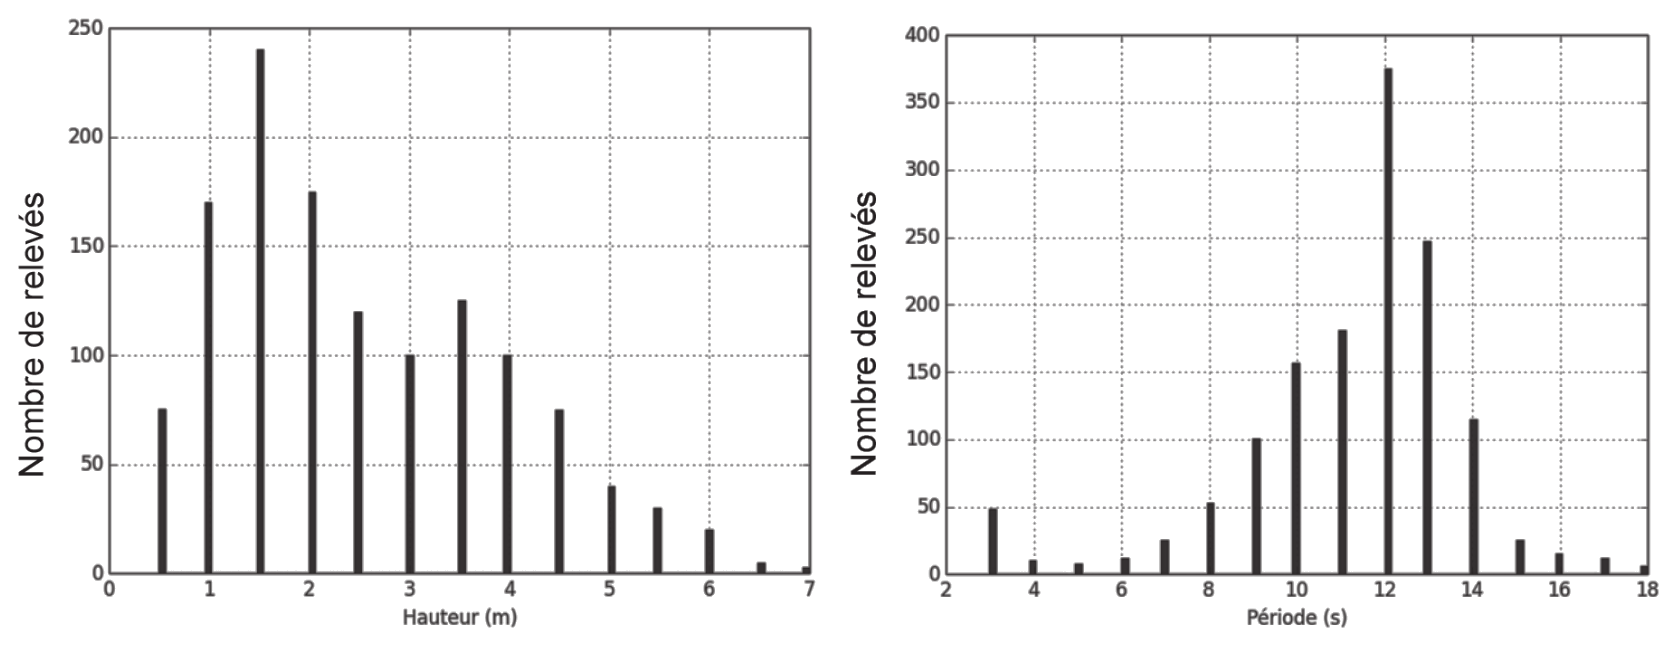
\includegraphics[width=0.85\linewidth]{img/fig07}
  \end{center}
  \caption{Répartition des relevés de la hauteur et de la période de houle du mois d'octobre}
\label{fig07}
\end{figure}

\question{En considérant le système houlomoteur comme un filtre dans le domaine fréquentiel, donner la bande passante: $[\omega_{min},\omega_{max}]$
 (en \SI{}{rad s^{-1}}) du système afin qu'il capte convenablement la houle correspondant à 50 relevés au moins. Préciser la pulsation dominante $\omega_n$.}
 
Durant la conception du système les quatre configurations de houle présentées dans le tableau \ref{tab01}, ont été retenues comme étant représentatives des phases de production d'énergie. Les puissances inférieures à l'état 1 seront généralement insuffisantes à la production d'énergie. Les amplitudes de houle supérieures à 4 mètres conduiront à une mise en sécurité du système.

\begin{table}
\begin{center}
\begin{tabular}{|c|c|c|c|}
\hline
Configurations de & Hauteur & Période & Puissance maximale\\
houle & H (m) & T (s) & (kW)\\
\hline
État 1 & 1,0 & 8,0 & 13,5 \\
\hline
État 2 & 2,0 & 10,0 & 67,3 \\
\hline
État 3 & 3,0 & 12,0 & 181,7 \\
\hline
État 4 & 4,0 & 14,0 & 376,9 \\
\hline
\end{tabular}
\end{center}
  \caption{Paramètres associés aux états représentatifs des phases de production d'énergie}
\label{tab01}
\end{table}

\subsection{Démarche de modélisation multiphysique}

Afin d'identifier et de valider les paramètres permettant au système de capter l'énergie houlomotrice, une modélisation complète multiphysique de l'ensemble est nécessaire. Le schéma de principe du modèle est donné figure \ref{fig08}.

\begin{figure}[ht!]
\begin{center}
  \def\svgwidth{0.95\linewidth}
  \input{img/fig08.pdf_tex}
 \end{center}
  \caption{Modèle multiphysique}
\label{fig08}
\end{figure}

On modélisera dans un premier temps le comportement hydrodynamique du flotteur sous l'effet de la houle afin de valider sa capacité à capter et transmettre l'énergie de manière optimale au système de conversion d'énergie.

On modélisera dans un second temps le système de conversion d'énergie afin de vérifier et d'optimiser les paramètres influant sur la quantité d'énergie produite.

Les modèles de comportement du flotteur et du système de conversion d'énergie sont liés par l'action résistante appliquée par le dispositif de conversion sur la bouée. Un modèle multiphysique (figure \ref{fig08}) liant les deux modèles précédents sera utilisé pour les simulations du comportement global du système.

\subsection{Modélisation hydrodynamique et validation des dimensions du flotteur}

Hypothèses et données (figure 4, page 3 et tableau 2, page 7) :
\begin{itemize}
 \item sous l'effet de la houle, le flotteur est animé d'un mouvement de translation selon la direction verticale $\vec{z}$, paramétré par le déplacement $z(t)$ par rapport à la position d'équilibre.
L'ensemble lest contenant le système de conversion d'énergie est considéré fixe par rapport au référentiel terrestre supposé galiléen ;
 \item on se placera dans les conditions de Heaviside (conditions initiales nulles) ;
 \item la théorie des vagues linéaires s'applique pour l'étude des actions de la houle sur le flotteur, on peut alors décomposer les actions de la houle sur le flotteur en la somme de trois actions :
 \begin{itemize}
 \item une force hydrostatique $\overrightarrow{f_{hs}(t)}$ incluant les actions du poids et de la poussée d'Archimède autour de la position d'équilibre $z = \SI{0}{\m}$:
 \begin{center}
	 $\overrightarrow{f_{hs}(t)}=-\rho\cdot g\cdot S\cdot z(t)\cdot\vec{z}$
 \end{center}
 \item une force d'excitation $\overrightarrow{f_{e}(t)}$ de la houle d'une hauteur $H$ et de pulsation $\omega$ s'exerçant sur un flotteur fixe :
 \begin{center}
	 $\overrightarrow{f_{e}(t)}=f_{e}(t)\cdot\vec{z}=-\rho\cdot g\cdot S\cdot \dfrac{H}{2}\cdot\sin(\omega\cdot t)\cdot\vec{z}$
 \end{center}
 \item une force de radiation $\overrightarrow{f_{r}(t)}$ s'exerçant sur un flotteur en mouvement dans un plan d'eau immobile:
  \begin{center}
	 $\overrightarrow{f_{r}(t)}=-A\cdot \ddot{z}(t)\cdot\vec{z}-B\cdot \dot{z}(t)\cdot\vec{z}$.
 \end{center}
 \end{itemize}
 \item l'action mécanique $\Phi(t)$ exercée par le vérin hydraulique sur le flotteur dépend des propriétés de l'ensemble du système de conversion d'énergie incluant le moteur hydraulique et la génératrice électrique. L'action de ce système de conversion d'énergie ramenée au vérin peut être modélisée globalement comme une action résistante proportionnelle à la vitesse de translation du vérin, faisant apparaître un coefficient d'amortissement équivalent noté C.

Cette action s'exprime :
  \begin{center}
	 $\overrightarrow{f_{v}(t)}=\Phi(t)\cdot\vec{z}=-C\cdot \dot{z}(t)\cdot\vec{z}$.
 \end{center}
La puissance mécanique captée par le système de conversion vaudra alors au maximum :
  \begin{center}
	 $P_{cap}=\dfrac{1}{2}\cdot C\cdot [\dot{z}(t)]^2$
 \end{center}
\end{itemize}

\begin{table}[ht!]
\begin{center}
\begin{tabular}{|c|c|c|}
\hline
Symbole & Désignation & Valeur numérique\\
\hline
$\rho$ & Masse volumique de l'eau & \SI{1 025}{\kg\m^{-3}}\\
\hline
$g$ & Accélération de la pesanteur & \SI{9,81}{\m\s^{-2}}\\
\hline
$S$ & Section du flotteur & \SI{12,58}{\m^2}\\
\hline
$m$ & Masse du flotteur & \multirow{2}{*}{m + A = \SI{53}{tonne}} \\
\cline{1-2}
$A$ & Masse additionnelle de radiation & \\
\hline
$B$ & Amortissement de radiation & \SI{80}{\kN\m^{-1}\s}\\
\hline
$H$ & Hauteur de houle & Variable\\
\hline
$C$ & Coefficient d'amortissement & Variable\\
 & équivalent & $C_{min}=$\SI{100}{\kN\m^{-1}\s}\\
\hline
$T$ & Période de la houle & Variable\\
\hline
\end{tabular}
\end{center}
  \caption{Données numériques pour la modélisation du flotteur}
\label{tab02}
\end{table}

L'application du théorème de la résultante du principe fondamental de la dynamique appliqué au flotteur donne l'équation suivante:
\begin{center}
$\left(\overrightarrow{f_{hs}}+\overrightarrow{f_{e}}+\overrightarrow{f_{r}}+\overrightarrow{f_{v}}\right)\cdot\overrightarrow{z}=m\ddot{z}$
\end{center}

\question{Montrer que l'on peut mettre l'équation différentielle du mouvement du flotteur paramétré par le déplacement z(t) sous la forme :
\begin{center}
 $a_2\cdot \ddot{z}(t)+a_1\cdot \dot{z}(t)+a_0\cdot z(t)=f_e(t)$
\end{center}

Donner l'expression algébrique des coefficients $a_i$ en fonction des données du tableau \ref{tab02}.}

\question{Déduire de la question précédente la fonction de transfert du flotteur, en fonction des coefficients $a_i$, donnant la transformée de Laplace du déplacement du flotteur $Z(p)=L[z(t)]$ à partir de la transformée de Laplace de l'action d'excitation $F_e(p)=L[f_e(t)]$:
\begin{center}
$H_{B}(p)=\dfrac{Z(p)}{F_e(p)}$
\end{center}}


\question{Déterminer l'expression algébrique puis numérique des paramètres caractéristiques de la fonction de transfert $H_B(p)$ (gain statique $K$, coefficient d'amortissement $\xi$ et pulsation propre non
amortie $\omega_0$ ) en fonction des données du tableau \ref{tab02} (on prendra $C=C_{min}$).}

\question{Tracer dans le plan de Bode sur le document réponse, le diagramme asymptotique de la fonction de transfert $\dfrac{H_B(p)}{K}$. Représenter l'allure du tracé réel.}

\question{Sur le document réponse faire apparaître la bande passante à - 6dB (plage des fréquences pour lesquelles le gain est supérieur à -6dB)  du flotteur. Conclure quant à la capacité du système à capter l'énergie de la houle pour la pulsation dominante $\omega_n$ déterminée à la question \ref{q5}.}

\subsection{Modélisation, validation et optimisation du système de conversion d'énergie}

Le système de conversion d'énergie est schématisé sur le document réponse, question \ref{q11}.

Le vérin hydraulique est entraîné par le mouvement relatif de translation entre le flotteur et le lest. La translation du piston par rapport au cylindre du vérin est donc également paramétrée par le déplacement $z(t)$ par rapport à la position d'équilibre. La section utile du piston est notée $S_p$. Les
pressions dans les chambres supérieure et inférieure du vérin sont notées respectivement $P_1$ et $P_2$.

Un réservoir accumulateur haute pression (a) et un réservoir accumulateur basse pression (b) permettent de maintenir les pressions $P_a$ (pression d'admission du moteur hydraulique) et $P_b$ (pression de refoulement du moteur hydraulique) quasi-constantes en régime établi.


\begin{wrapfigure}[8]{r}{0.25\textwidth}
	\vspace{-0.8cm}
\begin{center}
    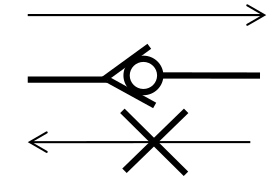
\includegraphics[width=0.8\linewidth]{img/fig09}
  \end{center}
    \caption{Schéma de principe des clapets}
\label{fig09}
\end{wrapfigure}


Un ensemble de clapets anti-retour permet de générer un débit volumique unidirectionnel $Q_m(t)$ vers le moteur hydraulique, quel que soit le sens de déplacement du piston. Le schéma et le principe des clapets anti-retour sont donnés sur la figure 

Les pertes induites par ce circuit redresseur seront négligées. On pourra alors considérer en régime établi, et en première approximation, les relations suivantes entre les pressions dans les réservoirs et dans les chambres du vérin : $P_a=max(P_1,P_2)$, $P_b=min(P_1,P_2)$.

\question{Compléter les zones en pointillés du schéma hydraulique du document réponse en dessinant les clapets anti-retour conformément à la description précédente.}

\subsubsection{Modélisation du système de contrôle de la cylindrée du moteur hydraulique}

Le moteur hydraulique employé dans le dispositif de conversion mécanique est un moteur à 9 pistons axiaux, à cylindrée variable. Nous allons chercher à modéliser la partie mécanique du dispositif de commande de la cylindrée et à valider la linéarité de son comportement.

Le principe de fonctionnement du moteur hydraulique est représenté sur le schéma cinématique de la figure \ref{fig10}.

Le débit volumique $Q_m(t)$ provenant du vérin hydraulique par l'intermédiaire du système redresseur (clapets anti-retour) alimente le moteur hydraulique. Ce débit provoque le déplacement axial des pistons $p_i$ par rapport au rotor 3 selon $\vec{z_0}$ ainsi que le glissement des pistons $p_i$ par rapport
au plateau 1, incliné d'un angle $\alpha (t)=(\vec{z_0},\vec{z_1})$. Le mouvement des pistons entraîne le rotor 3 du moteur hydraulique en rotation autour de l'axe $(O, \vec{z_0})$. La variation de cylindrée est réalisée en
modifiant l'amplitude du mouvement axial des pistons et donc en réglant l'inclinaison d'angle $\alpha$ du plateau 1. En effet, on peut montrer que le lien entre la cylindrée du moteur et l'inclinaison du plateau est donné par la relation : $x_m(\alpha)\cdot D_m=K_\alpha\cdot tan(\alpha)$ où $K_\alpha$ est une constante dépendant de la géométrie.

Le plateau 1 est entraîné en rotation autour de l'axe $(O,\vec{y_0})$
0 par un vérin de commande 2 lui-même piloté en translation de direction $\vec{x_0}$ par une servovalve hydraulique. Le déplacement du vérin de
commande 2 est paramétré par $\lambda (t)$.

\begin{figure}[ht!]
\begin{center}
  \def\svgwidth{0.65\linewidth}
  \input{img/fig10.pdf_tex}
 \end{center}
  \caption{Schéma cinématique du moteur hydraulique}
\label{fig10}
\end{figure}

Paramètres géométriques :
$\overrightarrow{OA}=r(t)\cdot\vec{z_1}$ \hfill
$\overrightarrow{IA}=-e\cdot\vec{z_0}$ \hfill
$\overrightarrow{HI}=\lambda(t)\cdot\vec{x_0}$ \hfill
$\overrightarrow{OH}=L\cdot\vec{z_0}$ \hfill
$\alpha(t)=(\vec{z_0},\vec{z_1})=(\vec{x_0},\vec{x_1})$

\question{Déterminer l'expression de $\lambda$ en fonction de $\alpha$, $L$ et $e$.}

\question{Déduire de la question précédente le paramètre $K_m$ tel que : $x_m(\alpha)\cdot D_m=K_m\cdot \lambda$. Conclure quant à la linéarité du mécanisme de commande de la cylindrée.}

\newpage

Le comportement dynamique du système de variation de la cylindrée du moteur peut être modélisé comme un système du premier ordre tel que :
\begin{center}
$H_{mh}(p)=\dfrac{X_m(p)}{X_{mC}(p)}=\dfrac{K_{mh}}{1+\tau_{mh}\cdot p}$, avec $K_{mh}=\SI{1}{}$ et $\tau_{mh}=\SI{0,1}{\s}$.
\end{center}

Où $X_m(p)=L[x_m(t)]$ est le facteur de commande de la cylindrée et $X_{mC}(p)=L[x_{mC}(t)]$ la consigne de facteur de commande de la cylindrée.

\subsubsection{Modélisation de la boucle d'asservissement de vitesse du moteur hydraulique}

Le schéma-bloc à retour unitaire de l'asservissement en vitesse du moteur hydraulique est présenté sur le document réponse, question \ref{q15}. L'écart en sortie de comparateur $\epsilon(p)=\omega_{mc}(p)-\omega_{m}(p)$ est corrigé par un correcteur à action proportionnelle et intégrale (PI), de fonction de transfert $C(p)$, qui génère une consigne de facteur de commande du débit $X_{mC}(p)$:
\begin{center}
$C(p)=\dfrac{X_{mc}(p)}{\epsilon(p)}=\dfrac{K_i}{p}+K_c$
\end{center}

\question{Compléter la zone en pointillés du schéma-bloc du document réponse en utilisant l'équation suivante (elle n'est pas à démontrer).}
\begin{center}
$J\cdot\dfrac{d\omega_m(t)}{dt}=-f{cg}\cdot\omega_m(t)+x_m(t)\cdot D_m\cdot\Delta P$
\end{center}

\newpage

Avec:
\begin{table}[ht!]
\begin{center}
\begin{tabular}{|c|c|c|}
\hline
Symbole & Désignation & Valeur numérique \\
\hline
$D_m$ & Cylindrée du moteur & \SI{60}{\cm^3 tr^{-1}}, soit \\
& & 9,55.10 -6 m 3 /rad \\
\hline
$x_m$ & Facteur de commande de la cylindrée &  $\in[0,1 ; 1]$\\
\hline
$f_{cg}$ & Facteur de couple variable de la &  Valeur maximale :\\
 & génératrice &  \SI{0,19}{\N\m rad^{-1}\s}\\
\hline
$J$ & Moment d'inertie &  \SI{2}{\kg\m^2} \\
\hline
$S_p$ & Section utile du piston &  \SI{0,007}{\m^2} \\
\hline
$P_a$ & Pression d'admission du moteur &  $P_{a,max}=\SI{350}{\bar}$\\
 & &  $P_{a,min}=\SI{30}{\bar}$\\
\hline
$P_b$ & Pression de refoulement du moteur &  $P_{b,min}=\SI{10}{\bar}$\\
\hline
\end{tabular}
\end{center}
  \caption{Données numériques pour la modélisation du système de conversion d'énergie}
\label{tab03}
\end{table}

\paragraph{Système non corrigé}~\ \\

On considère d'abord que $K_c=1$ et $K_i=0$.

\question{Sous ces hypothèses, déterminer la fonction de transfert en boucle ouverte FTBO(p) de l'asservissement en vitesse du moteur hydraulique sous forme canonique.}

\question{Donner l'expression de l'écart statique pour un échelon unitaire de vitesse de rotation. Est-ce conforme à l'exigence de précision ? Justifier alors la présence du correcteur PI dans le système.}

Le tracé de la fonction de transfert en boucle ouverte dans le plan de Bode pour $K_c=1$, $K_i=0$ et $\Delta P=\SI{100}{\bar}$ est donné sur le document réponse, question \ref{q19}.

\question{Déterminer la fonction de transfert correspondant au tracé de Bode du document réponse. Présenter directement sur le diagramme les constructions nécessaires à la démonstration.}

\newpage

\section{Lecture de plan}

\subsection{Palier de moteur électrique}

Les couvercles (1) et (2) immobilisent en translation la bague extérieure du roulement (4).

La liaison complète de ces deux couvercles avec la flasque (3) du moteur électrique est assurée par 3 vis CHC, M10, vissées de l'extérieur.

Les vis sont implantées dans le couvercle (2) sur toute l'épaisseur.

\begin{figure}[ht!]
\begin{center}
	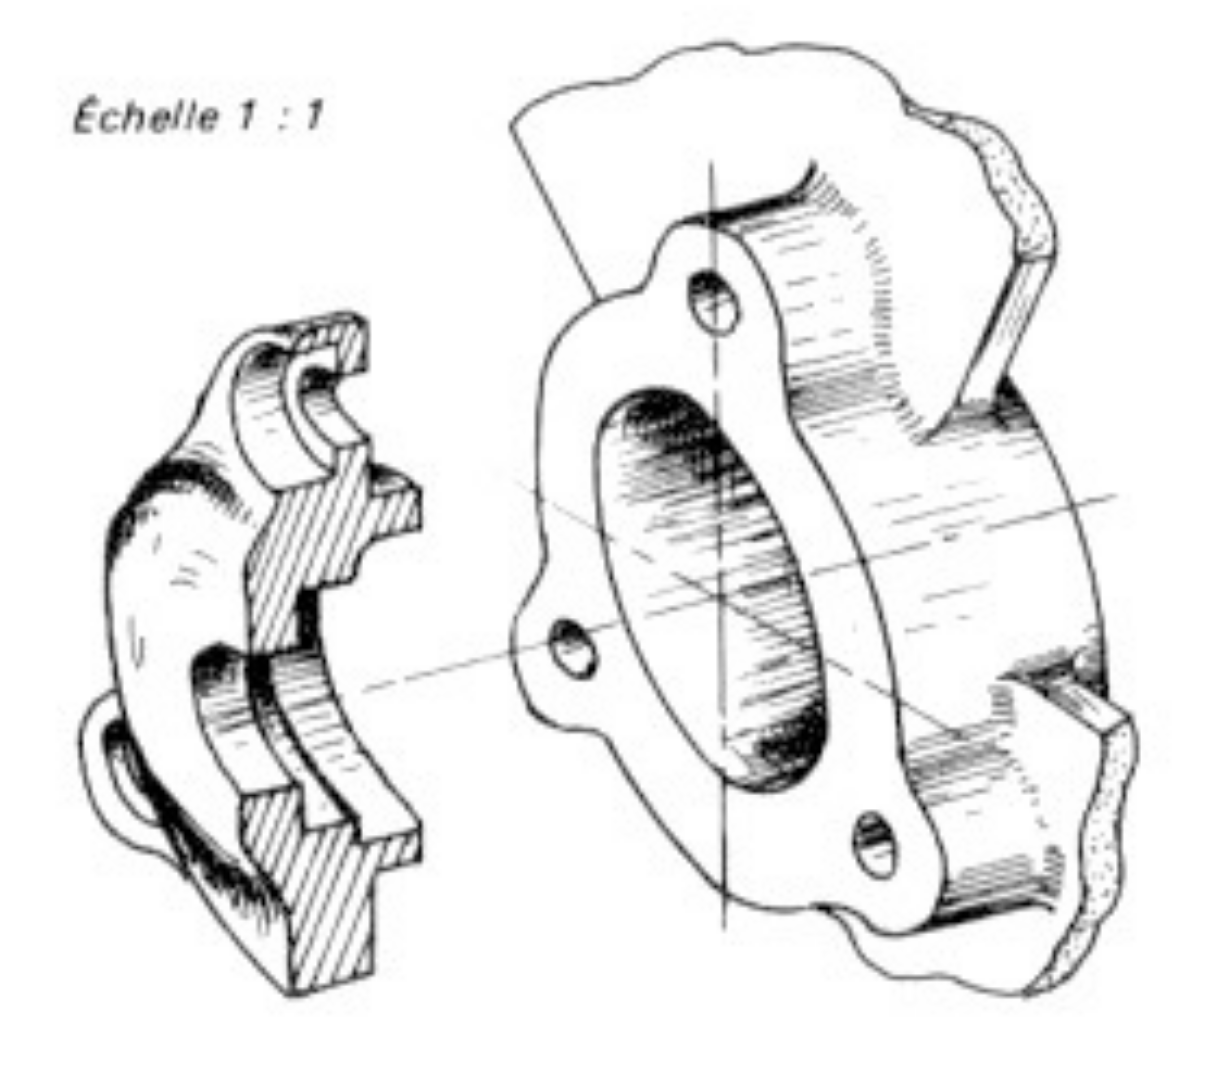
\includegraphics[width=0.3\linewidth]{img/dessin_01_pers}
\end{center}
  \caption{Vue en perspective d'un couvercle}
\label{fig11}
\end{figure}

\question{Mettre en place l'une de ces vis.}

\subsection{Cosse}

Sur la coupe du document réponse, à l'échelle 2.

\begin{figure}[ht!]
\begin{center}
	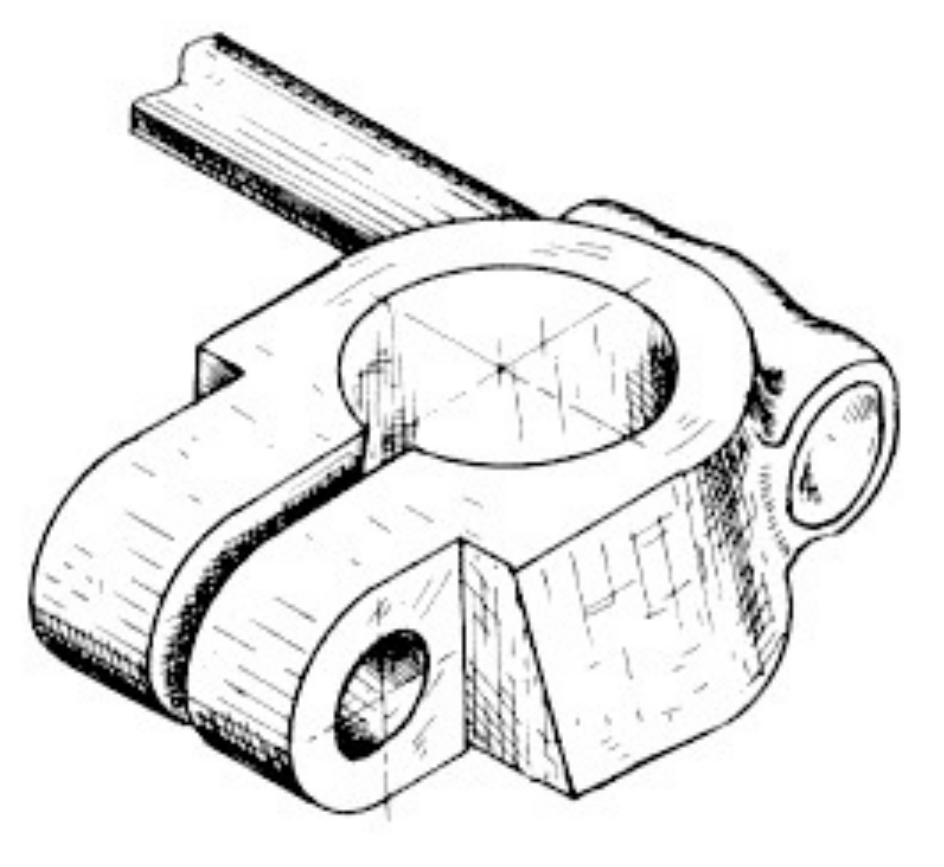
\includegraphics[width=0.3\linewidth]{img/dessin_02_pers}
\end{center}
  \caption{Vue en perspective de la cosse}
\label{fig12}
\end{figure}

\question{Mettre en place le boulon H, M8 établissant la liaison complète entre la borne (1) et la cosse (2).}

\question{Placer la tête du boulon vers le bas. Terminer la représentation du fraisage nécessaire à l'immobilisation en rotation de la tête du boulon.}

\cleardoublepage

\ifdef{\public}{\pagestyle{documentreponse}}{\pagestyle{correction}}

\reponse{4}{}{La poussée d’Archimède s'oppose au poids du volume d'eau déplacé, elle est donc:
\begin{itemize}
 \item verticale (+),
 \item elle correspond à la moitié du volume $0.5V_1$, car une seule moitié immergée,
 \item le poids de l'eau s'obtient en multipliant le volume par la masse volumique et l'accélération de pesanteur.
\end{itemize}}

\reponse{4}{}{$\overrightarrow{P_1}=-m_1~g\overrightarrow{z}$\\
$\overrightarrow{P_2}=-m_2~g\overrightarrow{z}$\\
$\overrightarrow{P_3}=-m_3~g\overrightarrow{z}$\\
$\overrightarrow{F_1}=0.5~\rho~V_1~g\overrightarrow{z}$\\
$\overrightarrow{F_2}=0.5~\rho~V_2~g\overrightarrow{z}$\\
$\overrightarrow{F_3}=0.5~\rho~V_3~g\overrightarrow{z}$}

\reponse{9}{}{$\left\{T_{P_1}\right\}=\left\{
\begin{array}{cc}
0 & 0\\
0 & 0\\
-m_1~g&0
\end{array}
\right\}_{G_1,B}$
$\left\{T_{P_2}\right\}=\left\{
\begin{array}{cc}
0 & 0\\
0 & 0\\
-m_2~g&0
\end{array}
\right\}_{G_2,B}$
$\left\{T_{P_3}\right\}=\left\{
\begin{array}{cc}
0 & 0\\
0 & 0\\
-m_3~g&0
\end{array}
\right\}_{G_3,B}$

$\left\{T_{F_1}\right\}=\left\{
\begin{array}{cc}
0 & 0\\
0 & 0\\
0.5~\rho~V_1~g&0
\end{array}
\right\}_{A_1,B}$
$\left\{T_{F_2}\right\}=\left\{
\begin{array}{cc}
0 & 0\\
0 & 0\\
0.5~\rho~V_2~g&0
\end{array}
\right\}_{A_2,B}$
$\left\{T_{F_3}\right\}=\left\{
\begin{array}{cc}
0 & 0\\
0 & 0\\
0.5~\rho~V_3~g&0
\end{array}
\right\}_{A_3,B}$

$\left\{T_{P_1}\right\}=\left\{
\begin{array}{cc}
0 & 0\\
0 & 0\\
-m_1~g&0
\end{array}
\right\}_{G_1,B}$
$\left\{T_{P_2}\right\}=\left\{
\begin{array}{cc}
0 & 0\\
0 & l_1~m_2~g\\
-m_2~g&0
\end{array}
\right\}_{G_1,B}$
$\left\{T_{P_3}\right\}=\left\{
\begin{array}{cc}
0 & 0\\
0 & l_2~m_3~g\\
-m_3~g&0
\end{array}
\right\}_{G_1,B}$

$\left\{T_{F_1}\right\}=\left\{
\begin{array}{cc}
0 & 0\\
0 & 0\\
0.5~\rho~V_1~g&0
\end{array}
\right\}_{G_1,B}$
$\left\{T_{F_2}\right\}=\left\{
\begin{array}{cc}
0 & 0\\
0 & -0.5~\rho~V_2~g~l_1\\
0.5~\rho~V_2~g&0
\end{array}
\right\}_{G_1,B}$

$\left\{T_{F_3}\right\}=\left\{
\begin{array}{cc}
0 & 0\\
0 & -0.5~\rho~V_3~g~l_2\\
0.5~\rho~V_3~g&0
\end{array}
\right\}_{G_1,B}$}

\ifdef{\public}{\newpage}

\reponse{4}{}{$-m_1~g-m_2~g-m_3~g+0.5~\rho~V_1~g+0.5~\rho~V_2~g+0.5~\rho~V_3~g=
-35000\times 10-120000\times 10-25000\times 10+0.5\times 1000\times 130\times 10+0.5\times 1000\times 60\times 10+0.5\times 1000\times 170\times 10=
-350000-1200000-250000+650000+300000+850000=0$

$l_1~m_2~g+l_2~m_3~g-0.5~\rho~V_2~g~l_1-0.5~\rho~V_3~g~l_2=
20\times 120000\times 10+30\times 25000\times 10-0.5\times 1000\times 60\times 10\times 20-0.5\times 1000\times 170\times 10\times 30=
24000000+7500000-6000000-25500000=(240+75-60-255=*100000=0$

Le système est bien à l'équilibre statique.}

\reponse{4}{}{Le volume immergé du lest est celui de 1, plus celui de 2, mais sans les \SI{4}{m} de lest qui sont hors de l'eau.

$V_im=V_1+V_2-\dfrac{\pi~d_2^2}{4}~4=130+60-\dfrac{3,14~1.5^2}{4}~4=130+60-\dfrac{7}{4}~4=183m^2$, on a donc la poussée d'Archimède $\overrightarrow{F_a}=V_im~\rho~g=183~1000~10=1830kN$.}

\reponse{4}{}{Le poids du système est la somme des poids de 1, de 2 et des ballasts.

$P_{total}=-(m_1+m_2+V_b~\rho)~g=-(155000+V_b~1000)~10=-1550-V_b~10kN$

Donc $V_b=\dfrac{(1830-1550)}{10}=\dfrac{280}{10}=28m^3<30m^3$.}

\reponse{4}{}{Les périodes mesurées sur au moins 50 relevés sont comprises entre 8 et 14 secondes.

La bande passante doit donc être $\left[\omega_{min},\omega_{max}\right]=\left[\dfrac{2~\pi}{14},\dfrac{2~\pi}{8}\right]=\left[0.44,0.79\right](rad/s)$.

La pulsation dominante correspond à une période de 12 secondes, c'est-à-dire $\omega_n=\SI{0.52}{rad s^{-1}}$.}


\reponse{4}{}{$-\rho\cdot g\cdot S\cdot z(t)+f_e(t)-A\cdot \ddot{z}(t)-B\cdot \dot{z}(t)-C\cdot \dot{z}(t)=m\ddot{z}$

$(m+A)\ddot{z}+(B+C)\cdot \dot{z}(t)+\rho\cdot g\cdot S\cdot z(t)=f_e(t)$

Donc, $a_2=m+A$, $a_1=B+C$ et $a_0=\rho\cdot g\cdot S$.}

\reponse{5}{}{$a_2\cdot p^2\cdot Z(p)+a_1\cdot p\cdot Z(p)+a_0\cdot Z(p)=F_e(p)$

$\left(a_2\cdot p^2+a_1\cdot p+a_0\right)\cdot Z(p)=F_e(p)$

$H_B(p)=\dfrac{Z(p)}{F_e(p)}=\dfrac{1}{a_2\cdot p^2+a_1\cdot p+a_0}$

$H_B(p)=\dfrac{Z(p)}{F_e(p)}=\dfrac{\dfrac{1}{a_0}}{\dfrac{a_2}{a_0}\cdot p^2+\dfrac{a_1}{a_0}\cdot p+1}$}

\reponse{9}{}{On identifie, $K=\dfrac{1}{a_0}=\dfrac{1}{\rho\cdot g\cdot S}=\dfrac{1}{1000\cdot 10\cdot 12.5}=\dfrac{1}{1000\cdot 1000\cdot 0.125}=8.10^{-6} N^{-1}.m$

$\omega_0=\sqrt{\dfrac{a_0}{a_2}}=\sqrt{\dfrac{\rho\cdot g\cdot S}{m+A}}=\sqrt{\dfrac{1}{8\cdot 10^{-6}\cdot 50000}}=\sqrt{\dfrac{1}{0.4}}=\sqrt{2.5}=\dfrac{5}{\sqrt{10}}=\dfrac{5}{3}=1.66 rad.s^{-1}$

$\xi=\dfrac{1}{2}\cdot\dfrac{a_1}{a_0}\cdot \sqrt{\dfrac{a_0}{a_2}}=\dfrac{a_1}{2\cdot \sqrt{a_0\cdot a_2}}$

$\xi=\dfrac{B+C}{2\cdot \sqrt{\rho\cdot g\cdot S\cdot (m+A)}}=\dfrac{180\cdot 10^3}{2\cdot \sqrt{\dfrac{50\cdot 10^3}{8.10^{-6}}}}=\dfrac{90\cdot 10^3}{\sqrt{\dfrac{50\cdot 10^9}{8}}}=\dfrac{90\cdot 10^3}{\sqrt{\dfrac{5}{8}}\cdot 10^5}=\dfrac{9}{\sqrt{\dfrac{5}{2}}\cdot 5}=\dfrac{9}{1.66\cdot 5}=\dfrac{9}{8.2}=\dfrac{8.2+0.8}{8.2}=1.1$}

\ifdef{\public}{\newpage}


\reponse[2]{0}{\begin{center}
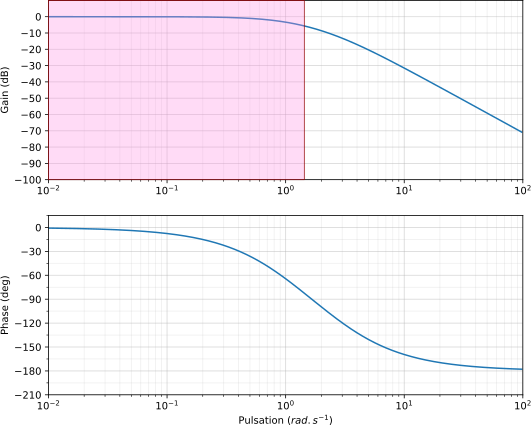
\includegraphics[width=0.9\linewidth]{img/bode01}
\end{center}}{\begin{center}
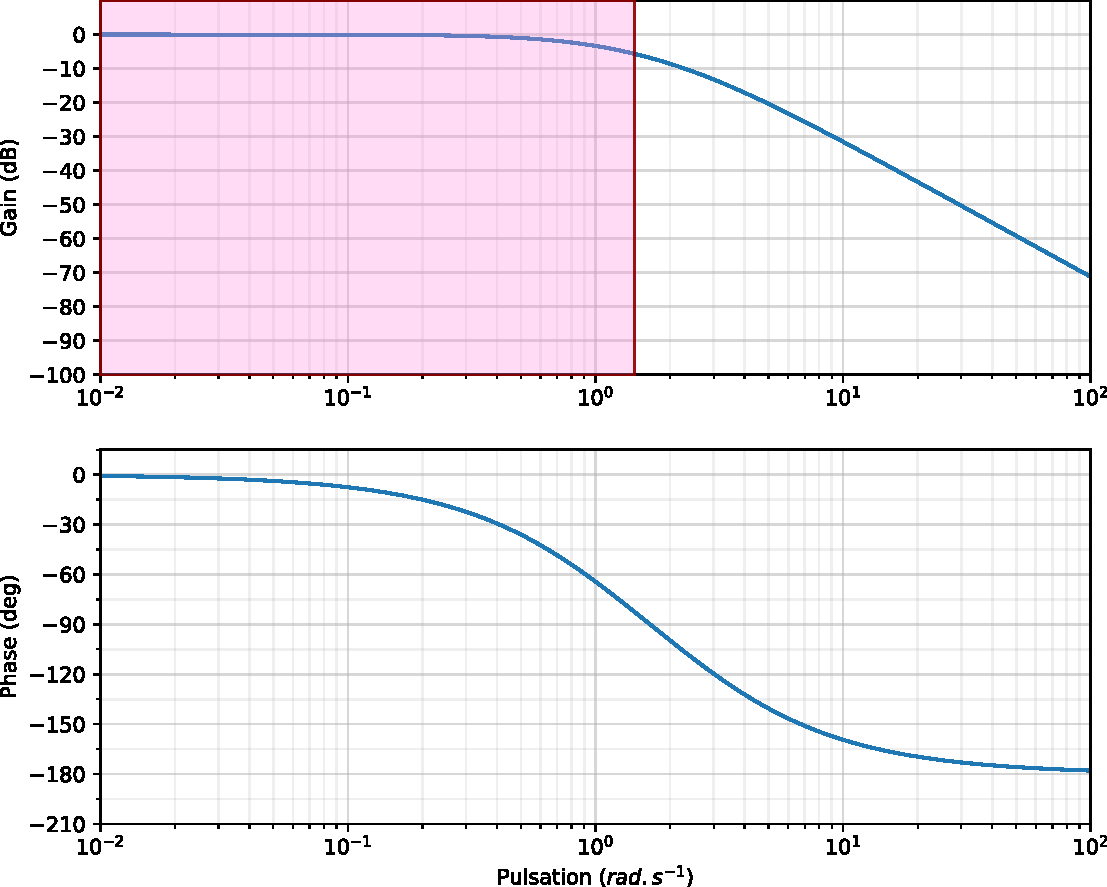
\includegraphics[width=0.9\linewidth]{img/bode01_cor}
\end{center}
Comme il s'agit d'un second ordre avec $\xi$ proche de 1, on sait que $G(\omega_0)$ est proche de -6dB par rapport à l'asymptote horizontale. Donc, le gain est supérieur à -6dB pour $\omega\in\left]0,\omega_0\right]$. $\omega_n$ est bien inclus dans cette bande passante.
}

\reponse{0}{\begin{center}
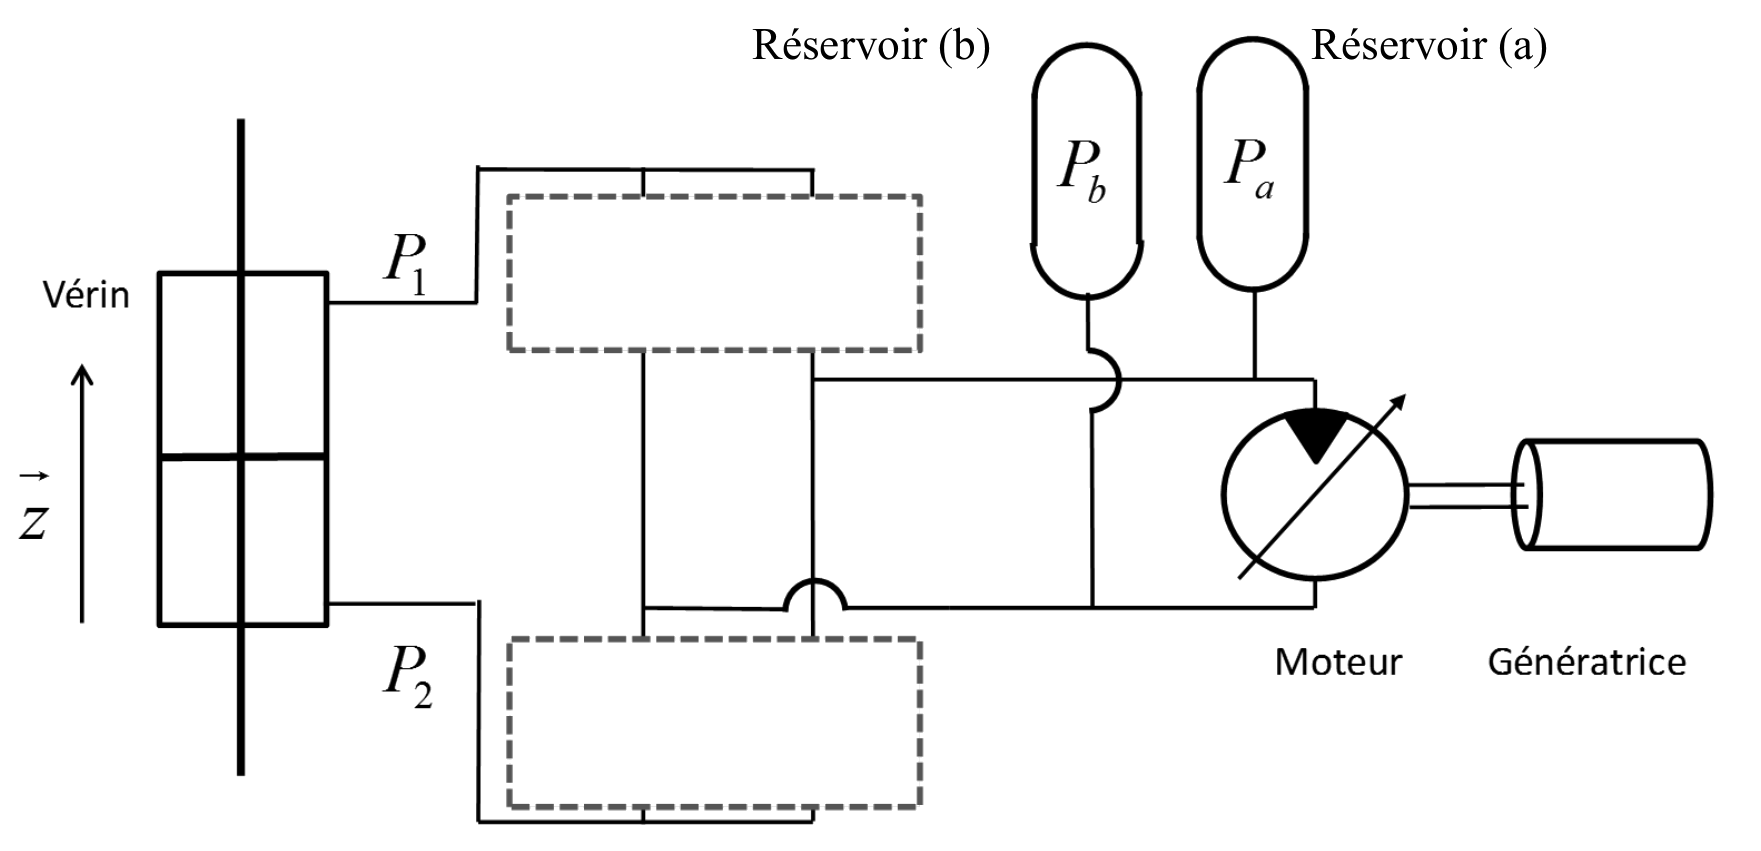
\includegraphics[width=0.85\linewidth]{img/hydraulique}
\end{center}}{\begin{center}
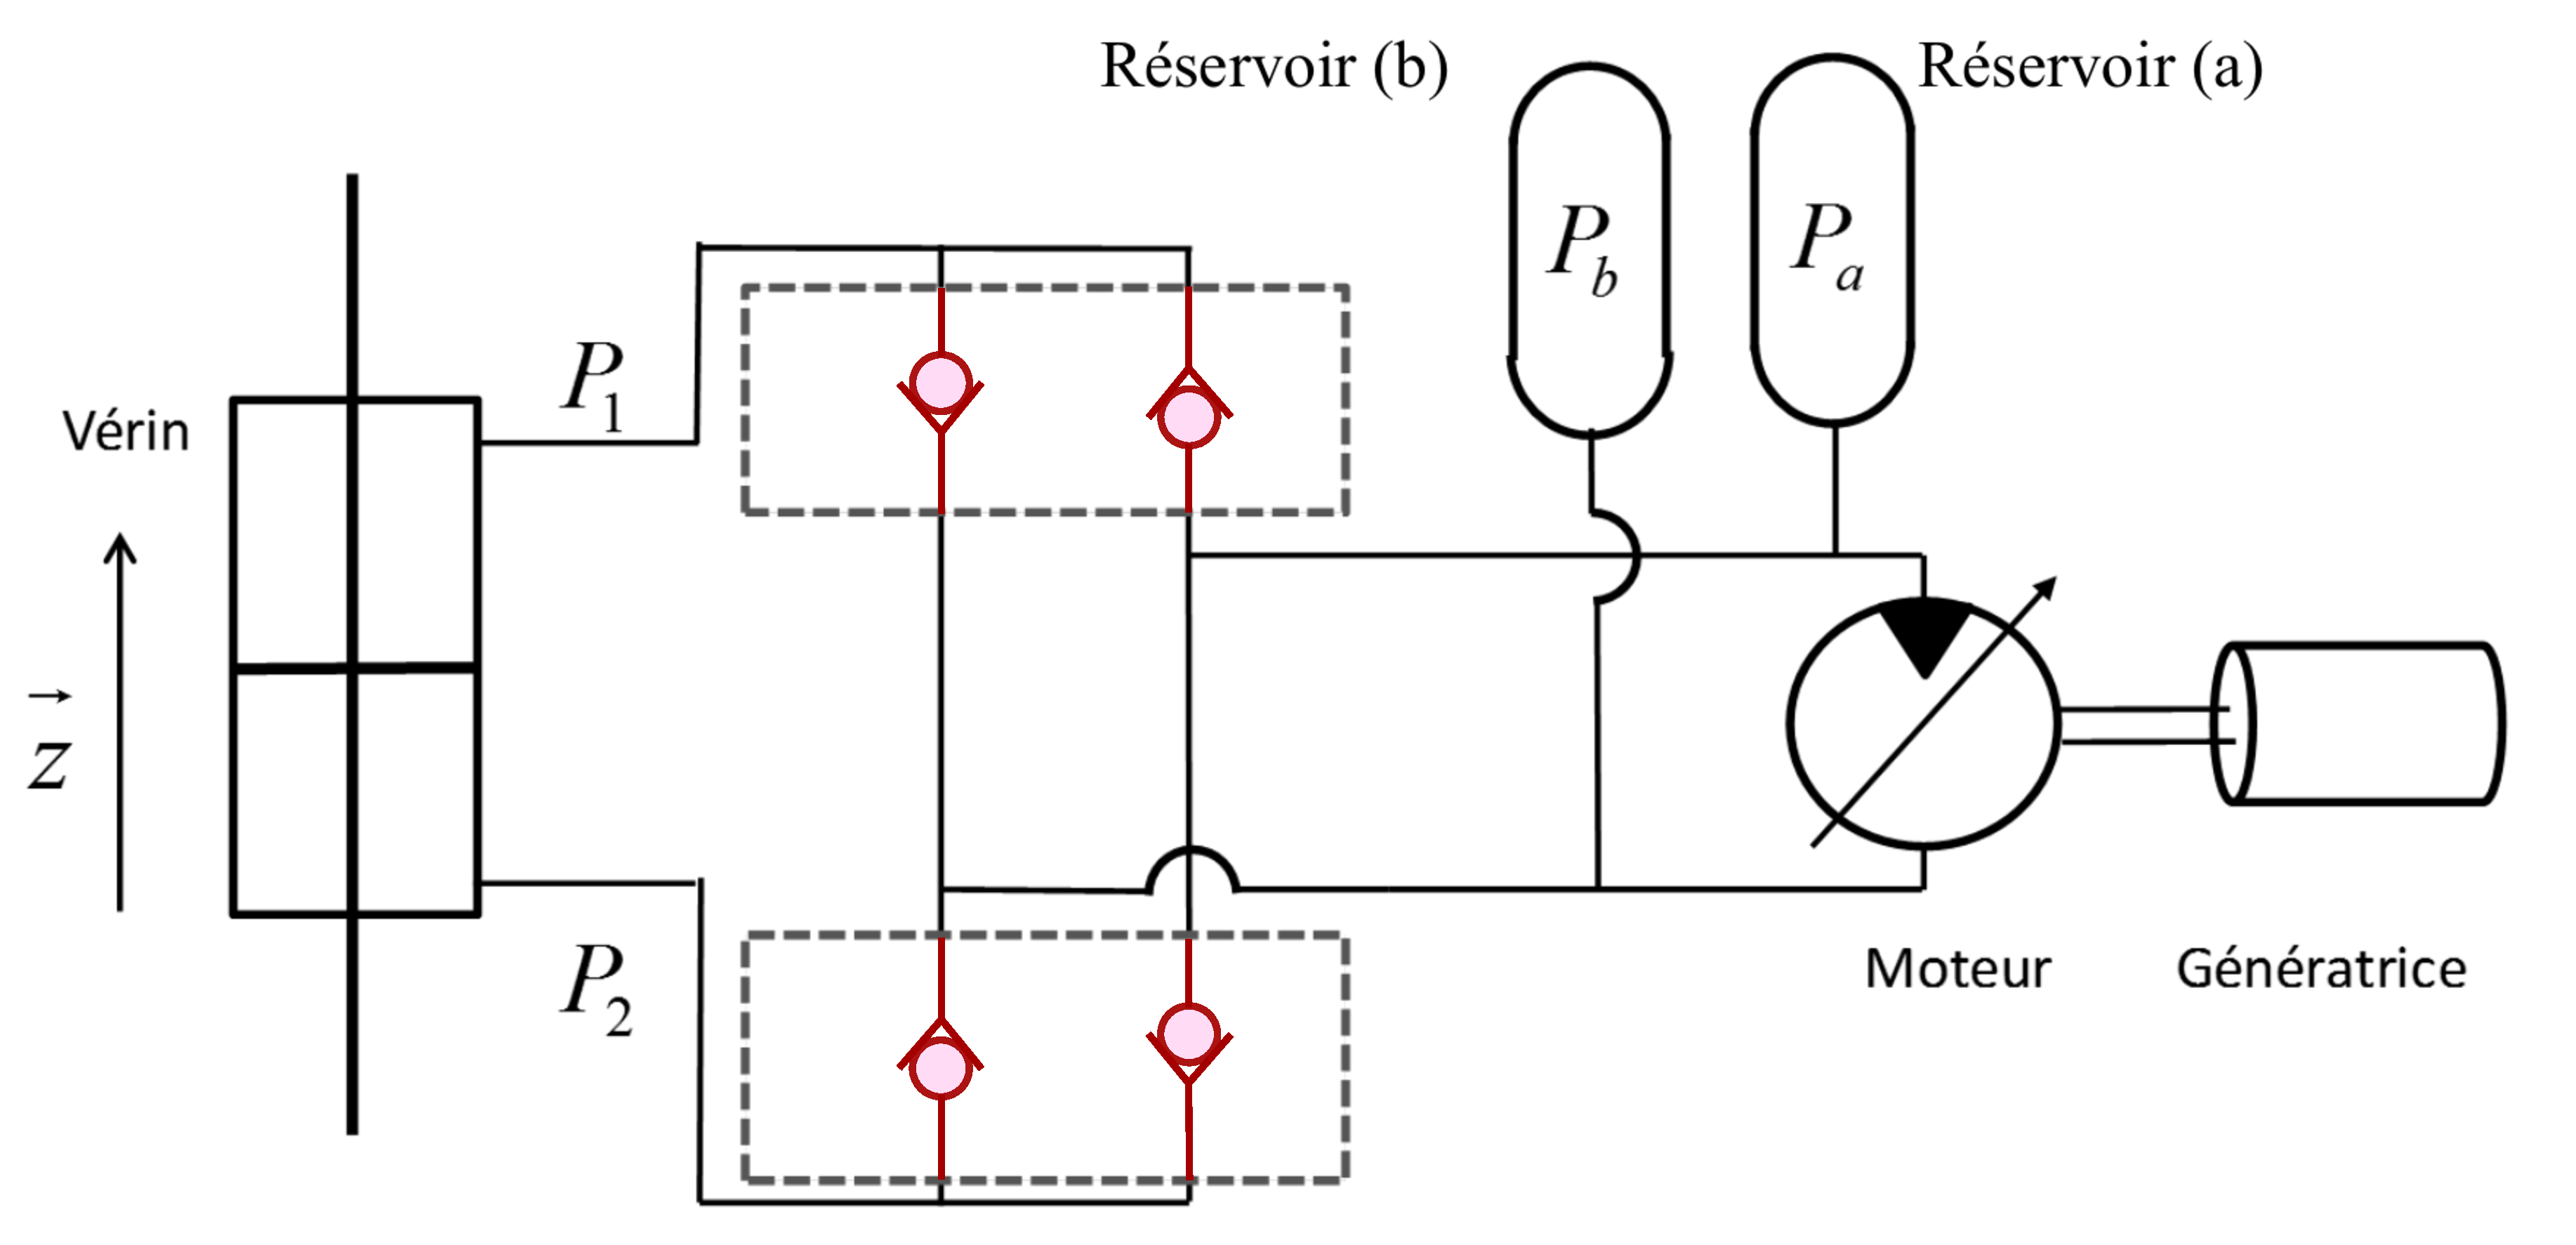
\includegraphics[width=0.85\linewidth]{img/hydraulique_cor}
\end{center}
Si $P_1$ augmente mouvement vers le haut, alors $P_2$ diminue et donc $P_a$ doit être connecté à $P_1$ et $P_b$ à $P_2$.
Dans le cas d'un mouvement de descente, c'est l'inverse.
}

\ifdef{\public}{\vspace{-2cm}}

\reponse{4}{}{Fermeture géométrique: $\overrightarrow{OA} + \overrightarrow{AI} + \overrightarrow{IH} + \overrightarrow{HO} = \overrightarrow{0}$

$r\cdot \overrightarrow{z_1}+ e\cdot \overrightarrow{z_0}-\lambda\cdot \overrightarrow{x_0} -L\cdot \overrightarrow{z_0} =\overrightarrow{0}$

\begin{itemize}
 \item sur $\overrightarrow{x_0}$ : $r~sin\alpha-\lambda = 0$ \\
 \item sur $\overrightarrow{z_0}$ : $r~cos\alpha + e-L = 0$
\end{itemize}

Donc, $\lambda=(L-e)tan\alpha$}

\reponse{4}{}{$x_m(\alpha)\cdot D_m=K_\alpha\cdot tan(\alpha)=K_m\cdot \lambda)$

Donc, $K_m=\dfrac{K_\alpha\cdot tan(\alpha)}{\lambda}=\dfrac{K_\alpha\cdot tan(\alpha)}{(L-e)\cdot tan(\alpha)}=\dfrac{K_\alpha}{L-e}$

$K_m$ étant constant, on a ainsi une preuve de la linéarité du mécanisme de commande de la cylindrée.}

\reponse{4}{\begin{center}
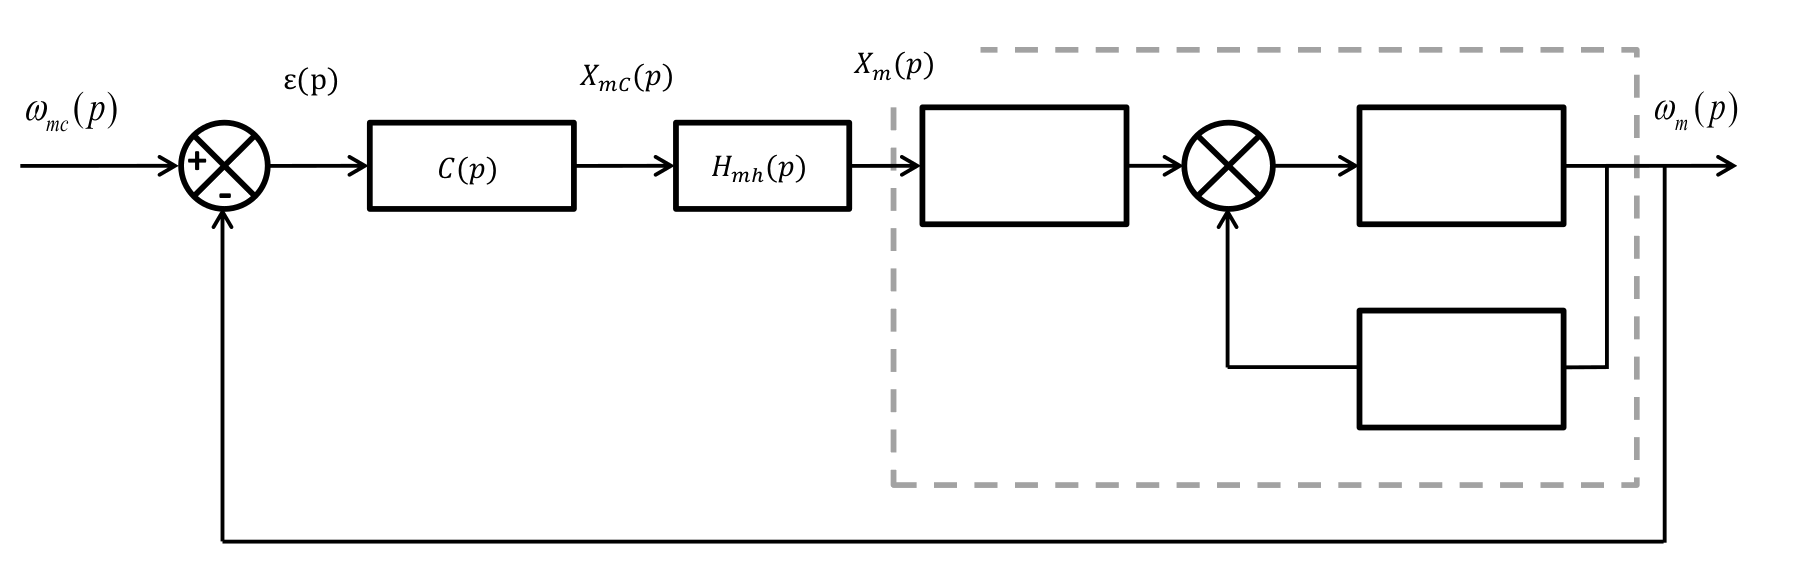
\includegraphics[width=0.9\linewidth]{img/schemabloc}
\end{center}}{\begin{center}
  \def\svgwidth{0.65\linewidth}
  \input{img/schemabloc_cor.pdf_tex}
\end{center}
Laplace: $Jp\Omega_m(p)=-f_{cg}\Omega_m(p)+X_m(p)D_m\Delta_p$

Donc, $\Omega_m(p)=\dfrac{1}{Jp}\left(X_m(p)D_m\Delta_p-f_{cg}\Omega_m(p)\right)$, ce qui permet de compléter les blocs du schéma.
}

\ifdef{\public}{\newpage}

\reponse{6}{}{
$FTBO(p)=C(p)\cdot H_{mh}(p)\cdot D_m\cdot \Delta_p\cdot\dfrac{\dfrac{1}{J\cdot p}}{1+\dfrac{1}{J\cdot p}\cdot f_{cg}}=\dfrac{K_{mh}}{1+\tau_{mh}p} \cdot D_m\cdot \Delta_p\cdot\dfrac{1}{Jp+ f_{cg}}$

Ce qui donne sous la forme canonique:
$FTBO(p)=\dfrac{K_{mh}\cdot D_m\cdot \Delta_p}{f_{cg}}
\dfrac{1}{(1+\tau_{mh}p)(1+\dfrac{J}{f_{cg}}p)}$
}


\reponse{6}{}{La classe étant nulle, on sait que l'écart statique sera non nul.

$e_s=\lim\limits_{x \to +\infty} \omega_{mc}(t)-\omega_m(t)$\\
$e_s=\lim\limits_{p \to 0} p\cdot\left(\omega_{mc}(p)-\omega_m(p)\right)$\\
$e_s=\lim\limits_{p \to 0} p\cdot\left(\omega_{mc}(p)-\dfrac{FTBO(p)}{1+FTBO(p)}\omega_{mc}(p)\right)$

Échelon unitaire en entrée, donc $\omega_{mc}(p)=\dfrac{1}{p}$

$e_s=\lim\limits_{p \to 0} p\cdot\left(1-\dfrac{FTBO(p)}{1+FTBO(p)}\right)\cdot\dfrac{1}{p}=\lim\limits_{p \to 0} \dfrac{1}{1+FTBO(p)}=\dfrac{1}{1+K_{BO}}$

Avec $K_{BO}=\dfrac{K_{mh}\cdot D_m\cdot \Delta_p}{f_{cg}}$.

Le cahier des charges n'est pas respecté, il faut donc mettre en place un correcteur PI.
}

\ifdef{\public}{\newpage}

\reponse{6}{\begin{center}
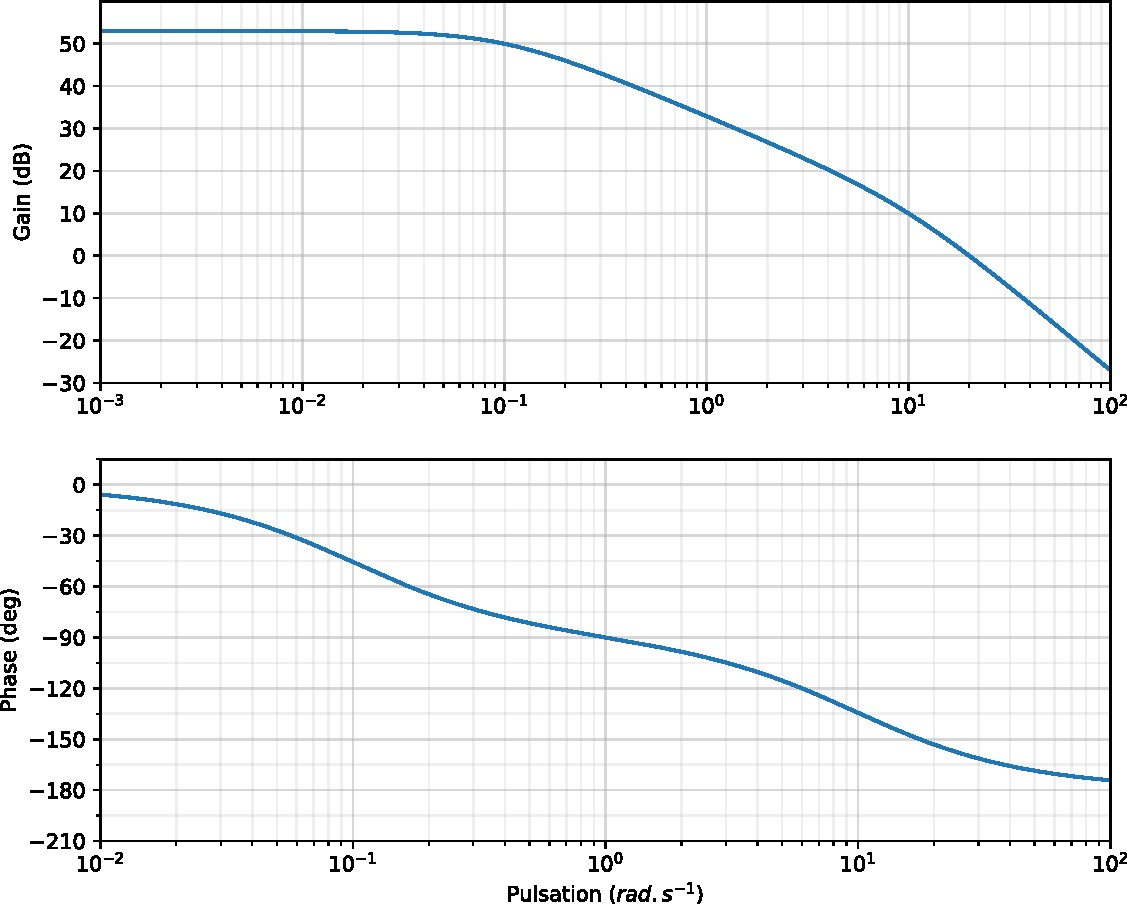
\includegraphics[width=0.9\linewidth]{img/bode02}
\end{center}}{\begin{center}
  \def\svgwidth{0.65\linewidth}
  \input{img/bode02_cor.pdf_tex}
\end{center}
$20log(K)=50$, donc $K=10^{2.5}=10^2\times 10^{0.5}\approx 100\times 3.1\approx 310$

$\omega_1=$\SI{0.1}{rad.s^{-1}}
$\omega_2=$\SI{10}{rad.s^{-1}}

La fonction de transfert est alors $\dfrac{K}{\left(1+\dfrac{p}{\omega_1}\right)\left(1+\dfrac{p}{\omega_2}\right)}$
}

\reponse{0}{\begin{center}
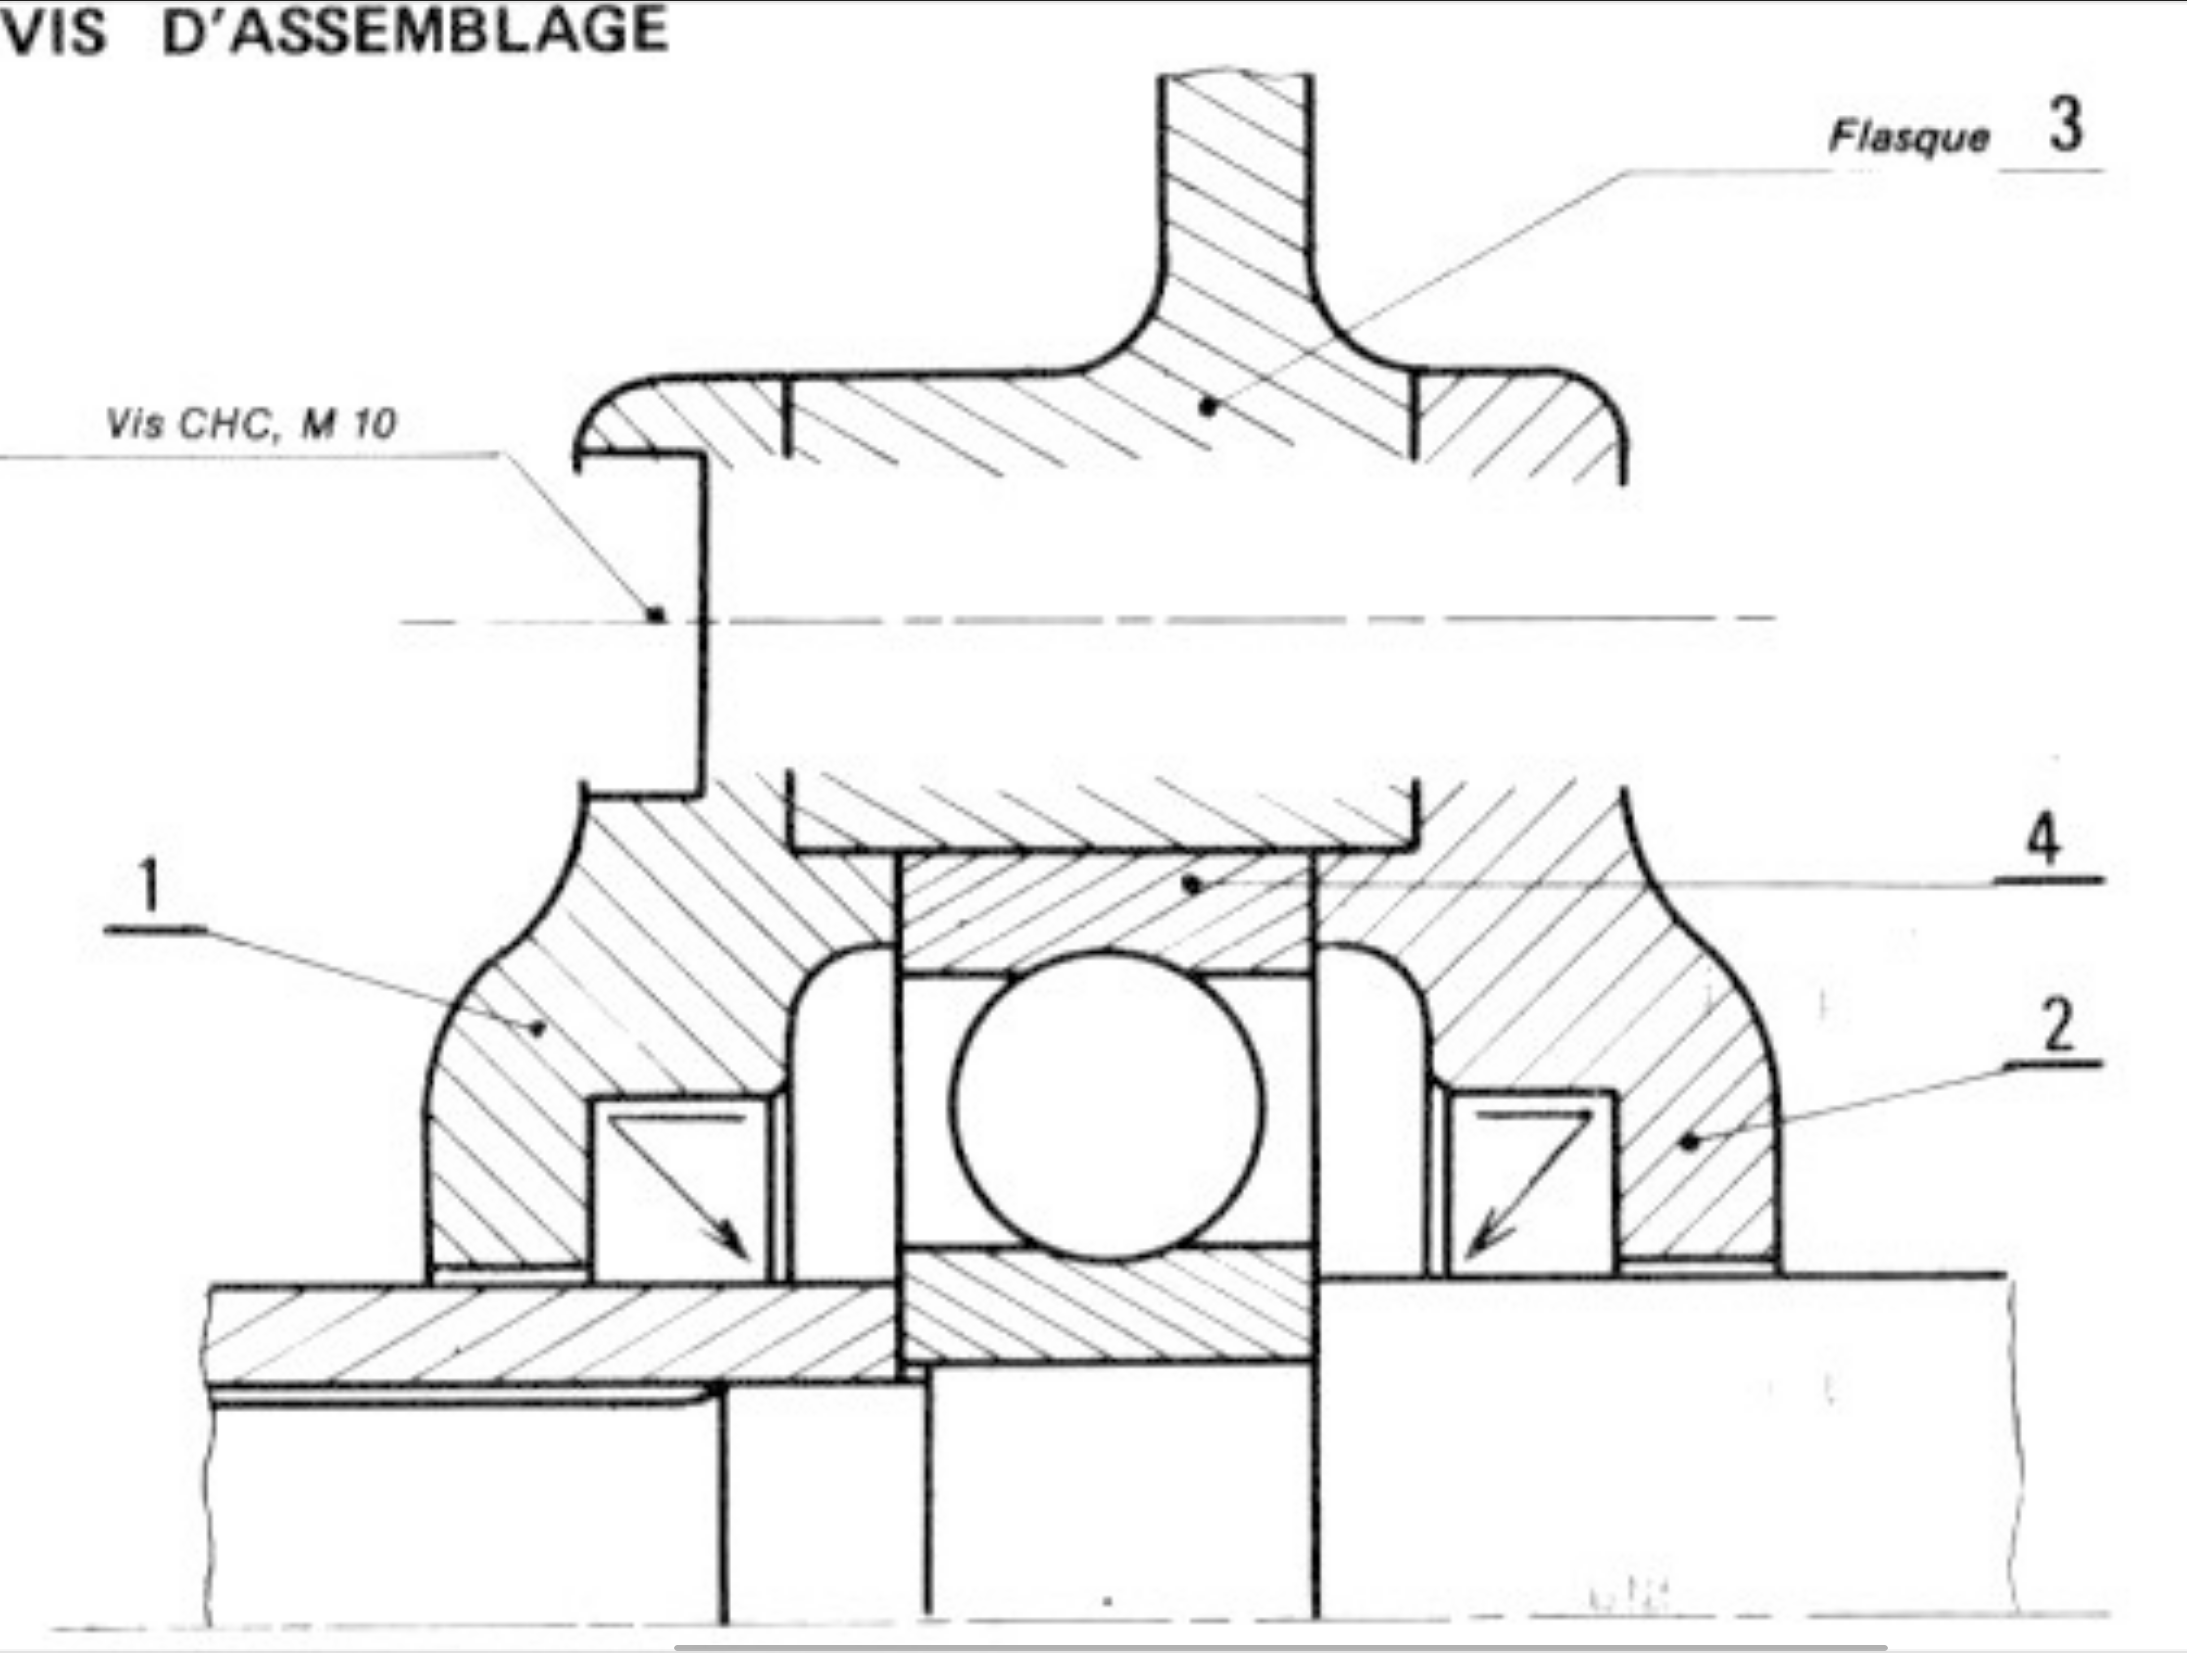
\includegraphics[width=0.85\linewidth]{img/dessin_01_dr}
\end{center}}{\begin{center}
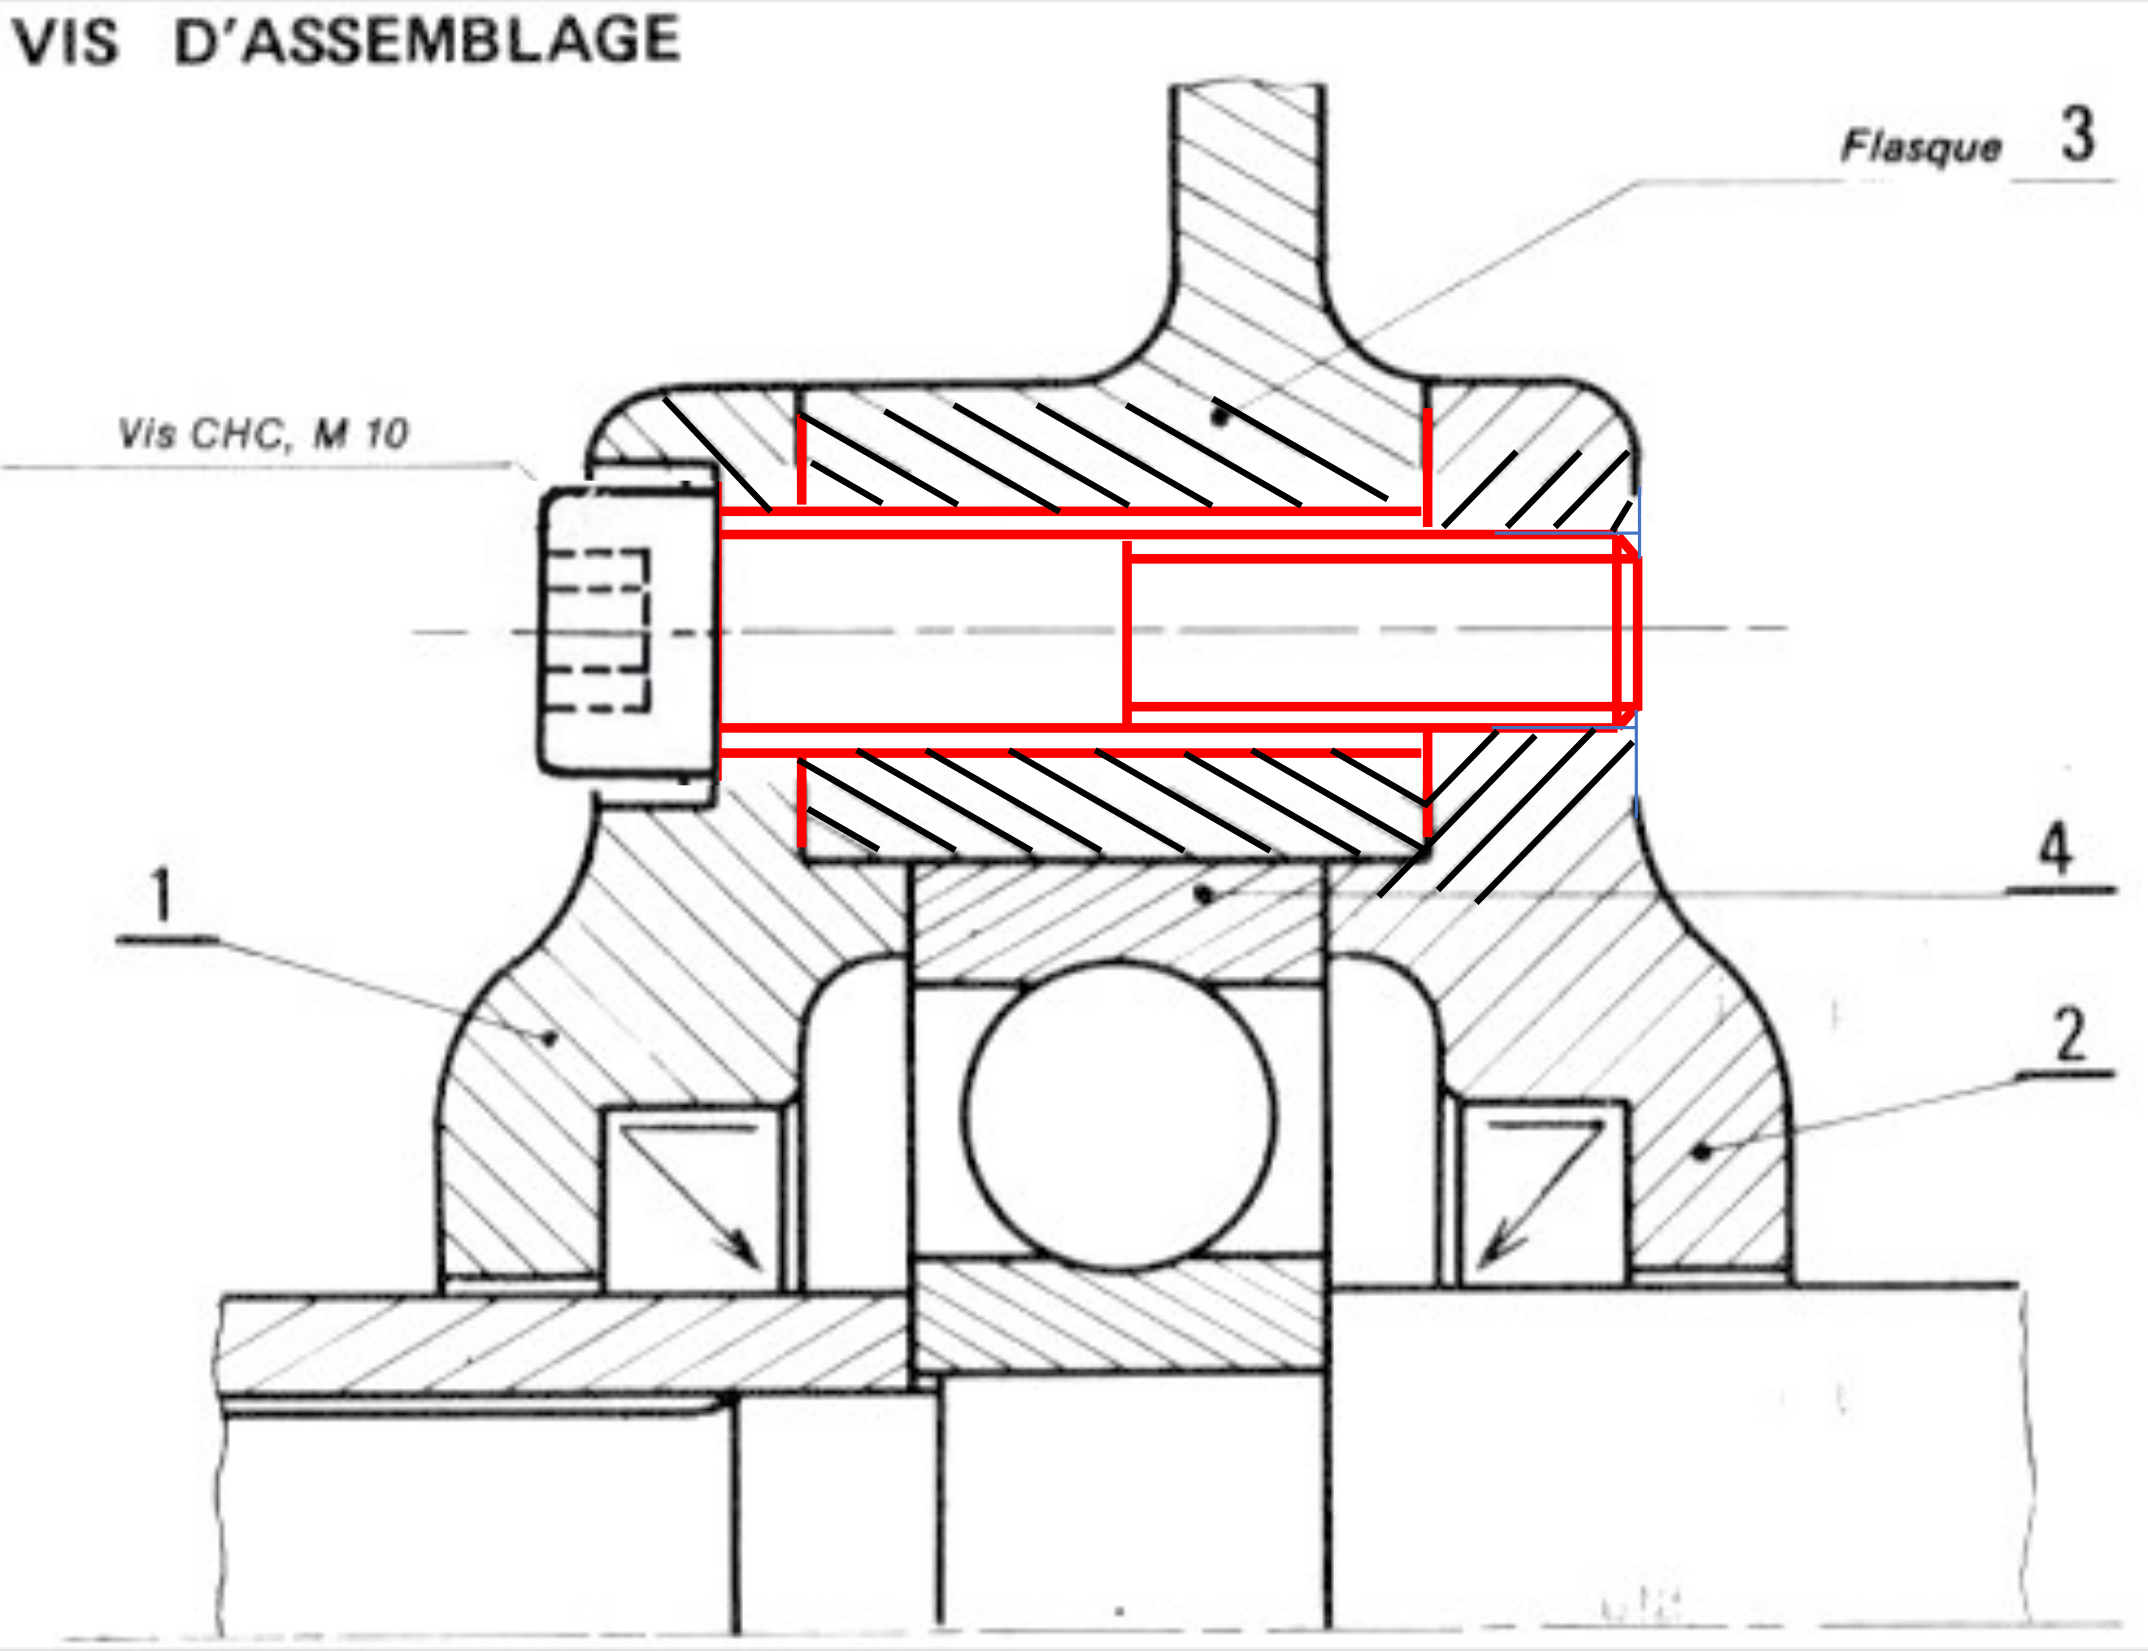
\includegraphics[width=0.85\linewidth]{img/dessin_01_cor}
\end{center}}

\reponse[2]{0}{\begin{center}
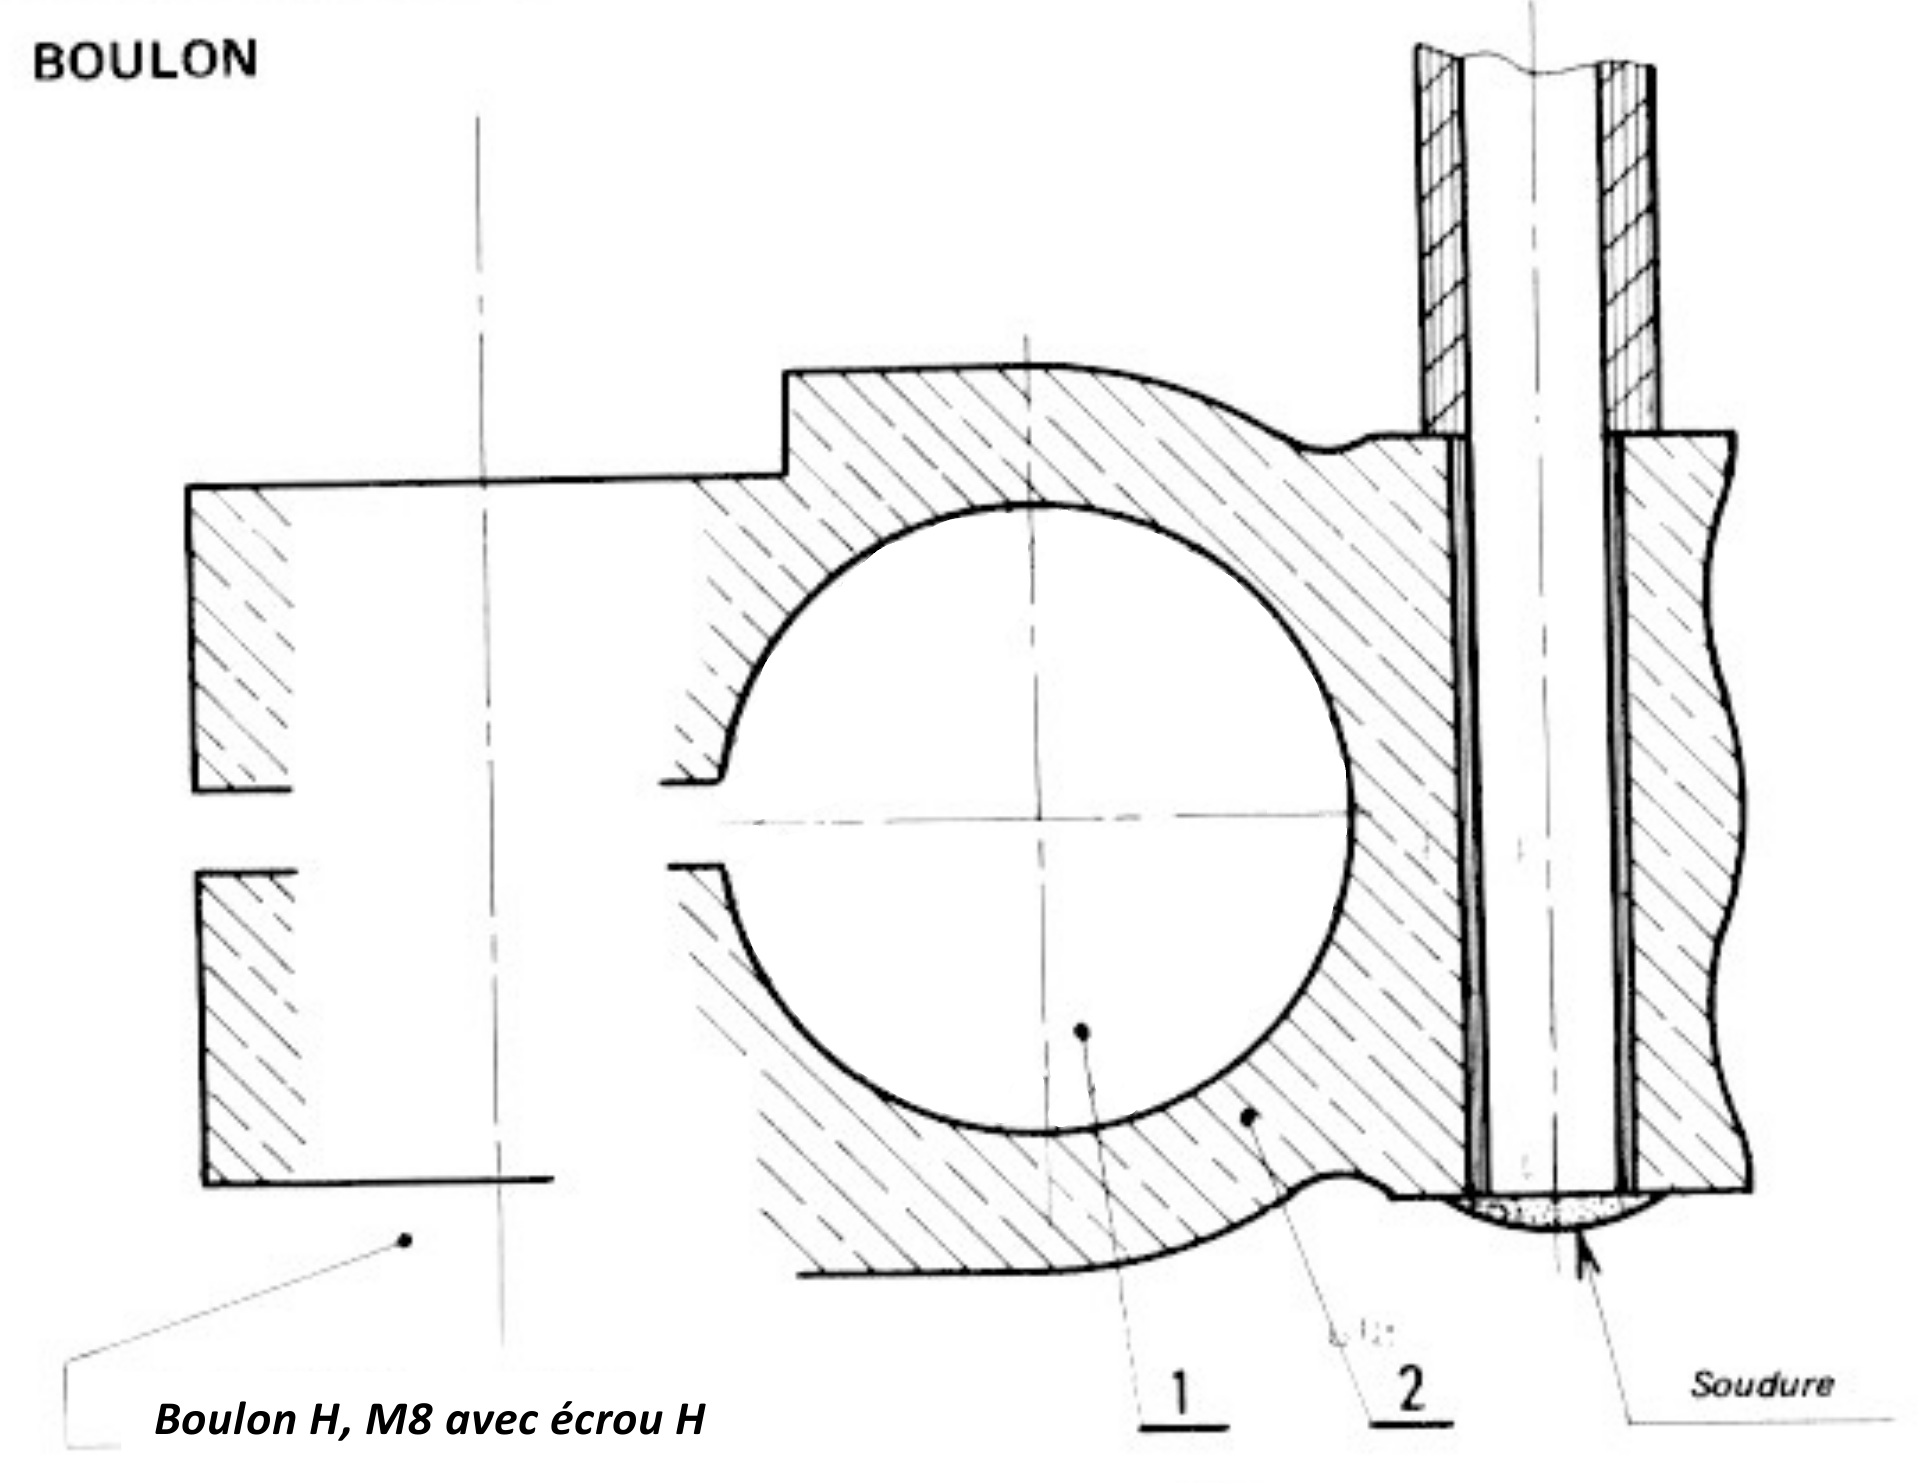
\includegraphics[width=0.85\linewidth]{img/dessin_02_dr}
\end{center}}{\begin{center}
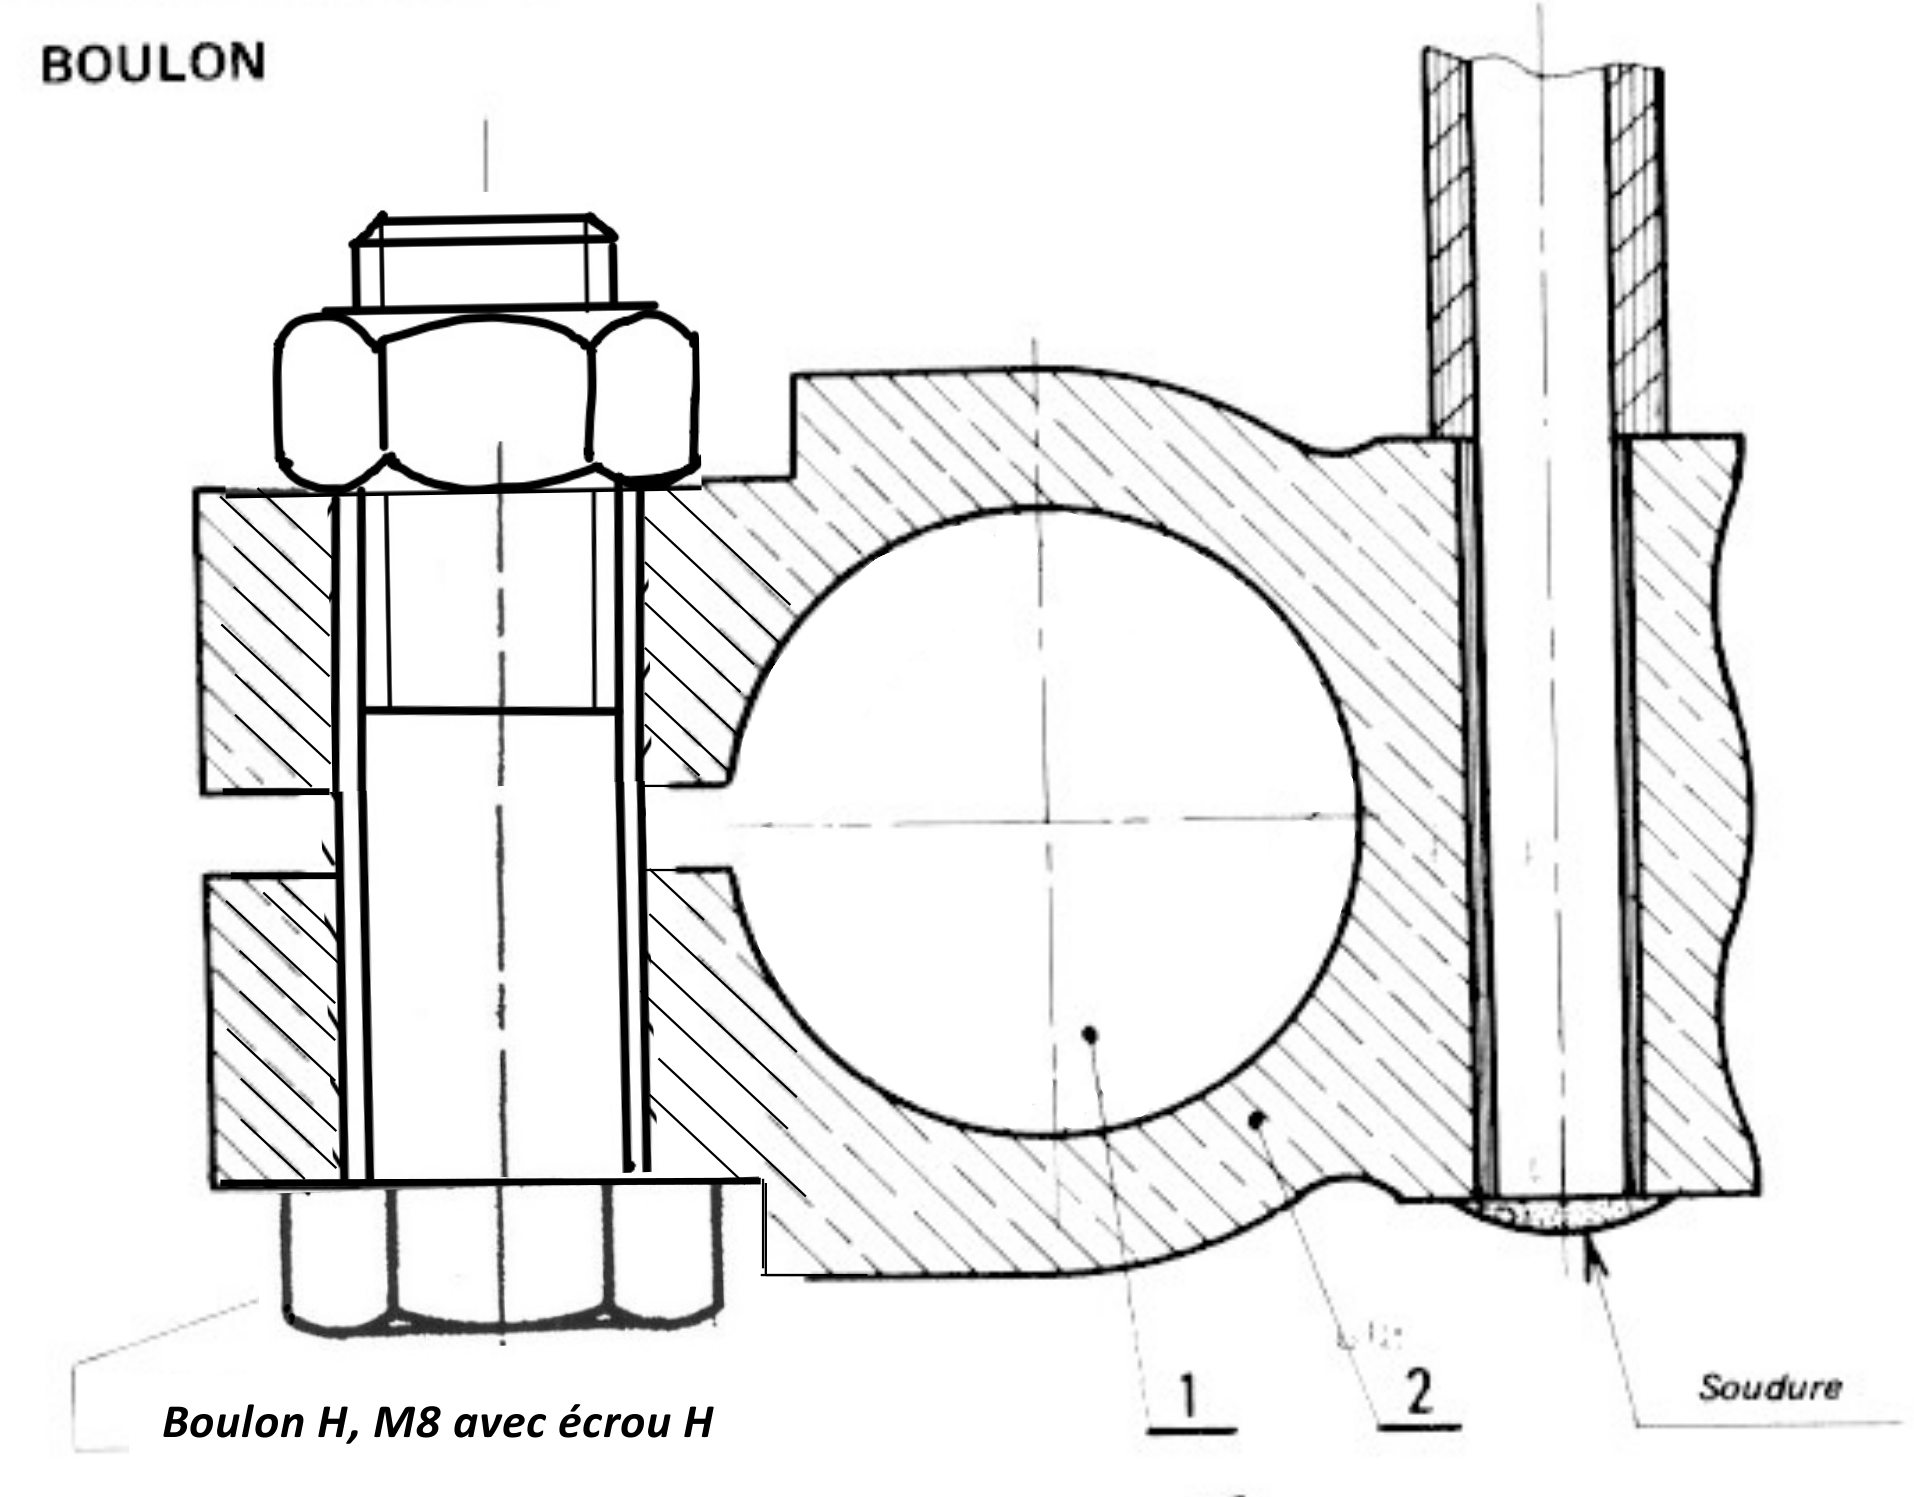
\includegraphics[width=0.85\linewidth]{img/dessin_02_cor}
\end{center}}


\end{document}